
\documentclass{article} % For LaTeX2e
\usepackage[final]{colm2025_conference}

% \usepackage[table]{xcolor}

\usepackage{microtype}
\usepackage{hyperref}
\usepackage{url}
\usepackage{booktabs}
\usepackage{enumitem}

\usepackage{lineno}
%Including images in your LaTeX document requires adding
%additional package(s)
\usepackage{graphicx}
\usepackage{caption}
\usepackage{booktabs}
\usepackage{tabularx}
\usepackage{pifont}
\usepackage{makecell} 
\usepackage{setspace}
\usepackage{multirow}
\usepackage{placeins}


\definecolor{darkblue}{rgb}{0, 0, 0.5}
\hypersetup{colorlinks=true, citecolor=darkblue, linkcolor=darkblue, urlcolor=darkblue}


% \title{\textit{\datasetname:} Benchmarking Personalized Memory in Large Language Models within Long Conversation History}
%\title{\textit{Hear Me, Know Me, Respond to Me}: \\ Benchmarking Personalized Memory and Response Generation in Language Agents.}
% \title{\textit{How much does your language model know about you?} \\ Benchmarking Personalized Memory in Large Language Models within Long Conversation History}
% \title{Is Your Language Model a Personalized Chatbot? \\ Benchmarking Memory and Personalized Generation at Scale}
% \title{\textit{How well does your LLM know you?}  Benchmarking Dynamic User Profiling and Personalized  Responses at Scale}
% \title{\textit{Do Language Models Really Know You?} \\ Benchmarking Dynamic User Profiling and Personalized \\ Response at Scale}
% \title{\textit{Know Me, Respond to Me:} \\ Benchmarking Memory and Personalized Generation at Scale}
\title{\textit{Know Me, Respond to Me:} Benchmarking LLMs for \\ Dynamic User Profiling and Personalized Responses at Scale}
% \title{\textit{Know Me, Reflect Me, Respond to Me:} \\ Benchmarking Memory and Personalized Generation at Scale}
% \title{Is Your Language Model a Personalized Chatbot? \\ Benchmarking Memory and Personalized Generation at Scale}
% Evaluating the Memorization of User Personas in Long Multi-Turn Conversations}
%\title{\textit{\datasetname:} Benchmarking Personalized Memory in Large Language Models within Multi-Turn Conversations}
% \title{\textit{\datasetname:} What do Large Language Models Know about Users from Conversation History}
% \title{MemoryBench: Evaluating the Memorization and Persona-Driven Generation in Long Conversations}
% \title{\textit{\datasetname:} Benchmarking LLMs's Memory of Personalized, Long-Form Conversations}


% Author information can be set in various styles:
% \author{Bowen Jiang\textsuperscript{1}\thanks{Equal first contribution, $^\dagger$equal second contribution},\ \ Zhuoqun Hao\textsuperscript{1}\footnotemark[1],\ \ Young-Min Cho\textsuperscript{1}$^\dagger$,\ \ Bryan Li\textsuperscript{1}$^\dagger$, Yuan Yuan\textsuperscript{1}$^\dagger$, \\ {\bf  Sihao Chen\textsuperscript{2}$^\dagger$,\ \ Lyle Ungar\textsuperscript{1}, Camillo J. Taylor\textsuperscript{1},\ \ Dan Roth\textsuperscript{1}} \\
\author{Bowen Jiang\textsuperscript{1}\thanks{Equal contribution},\ \ Zhuoqun Hao\textsuperscript{1}\footnotemark[1],\ \ Young-Min Cho\textsuperscript{1},\ \ Bryan Li\textsuperscript{1}, Yuan Yuan\textsuperscript{1}, \\ {\bf  Sihao Chen\textsuperscript{2},\ \ Lyle Ungar\textsuperscript{1}, Camillo J. Taylor\textsuperscript{1}\thanks{Equal advising},\ \ Dan Roth\textsuperscript{1}\footnotemark[2]} \\ 
University of Pennsylvania, Philadelphia, PA\textsuperscript{1} \\
Microsoft, Redmond, WA\textsuperscript{2} \\
\small{
\texttt{\{bwjiang, zhuoqunh, jch0, bryanli, yyuan86\}@upenn.edu}}\\
\small{
\texttt{sihaochen@microsoft.com, \{ungar, cjtaylor, danroth\}@upenn.edu}
}
}

\newcommand{\datasetname}{\textsc{PersonaMem}}
\newcommand{\datasetnameemoji}{
\includegraphics[height=1em]{figures/silhouette-emoji.png}~\textsc{PersonaMem}}
\newcommand{\personahub}{PersonaHub}

\newcommand\textbfblue[1]{\textcolor{darkblue}{\textbf{#1}}}


\usepackage[most]{tcolorbox}
\usepackage{tcolorbox}
\tcbuselibrary{theorems}

\newtcolorbox{prompt}[1]{
colback=green!5,colframe=green!35!black,fonttitle=\bfseries, title={#1}}

\begin{document}
\maketitle

% Authors must not appear in the submitted version. They should be hidden
% as long as the \colmfinalcopy macro remains commented out below.
% Non-anonymous submissions will be rejected without review.

% \author{Antiquus S.~Hippocampus, Natalia Cerebro \& Amelie P. Amygdale \thanks{ Use footnote for providing further information
% about author (webpage, alternative address)---\emph{not} for acknowledging
% funding agencies.  Funding acknowledgements go at the end of the paper.} \\
% Department of Computer Science\\
% Cranberry-Lemon University\\
% Pittsburgh, PA 15213, USA \\
% \texttt{\{hippo,brain,jen\}@cs.cranberry-lemon.edu} \\
% \And
% Ji Q. Ren \& Yevgeny LeNet \\
% Department of Computational Neuroscience \\
% University of the Witwatersrand \\
% Joburg, South Africa \\
% \texttt{\{robot,net\}@wits.ac.za} \\
% \AND
% Coauthor \\
% Affiliation \\
% Address \\
% \texttt{email}
% }

% The \author macro works with any number of authors. There are two commands
% used to separate the names and addresses of multiple authors: \And and \AND.
%
% Using \And between authors leaves it to \LaTeX{} to determine where to break
% the lines. Using \AND forces a linebreak at that point. So, if \LaTeX{}
% puts 3 of 4 authors names on the first line, and the last on the second
% line, try using \AND instead of \And before the third author name.

\newcommand{\fix}{\marginpar{FIX}}
\newcommand{\new}{\marginpar{NEW}}

\ifcolmsubmission
\linenumbers
\fi

\begin{abstract}

% Large Language Models (LLMs) are increasingly used as conversational chatbots, yet one key question remains: how well do they remember our interactions to deliver personalized responses?
% \textcolor{orange}{Sihao: The high-level framing of the story should be \textbf{**laser-focused** on personalization}, more specifically -- "\textbf{learning about each user from the user-LLM interaction history across different scenarios}". IMO we should avoid putting emphasis on "memory" or "long-context". Try to highlight our competitive advantage here -- (1). We have persona for user + user's entire (and diverse) interaction history w/ LLM, and (2). We are testing LLM in realistic task scenarios that require personalization.  }

% \textcolor{orange}{Research Questions
% \begin{enumerate}
%     \item User profiling: Can LLM learn about users from interaction histories?
%     \item Dynamic: Can LLM recognize how user preferences evolve over time?
%     \item Personalized response: Can LLM use what it knows about user and personalize its response?
% \end{enumerate}}
Large Language Models (LLMs) have emerged as \textit{personalized} assistants for users across a wide range of tasks -- from offering writing support to delivering tailored recommendations or consultations. Over time, the interaction history between a user and an LLM can provide extensive information about an individual's traits and preferences. However, open questions remain on how well LLMs today can effectively leverage such history to (1) internalize the user's inherent traits and preferences, (2) track how the user profiling and preferences evolve over time, and (3) generate personalized responses accordingly in new scenarios.

In this work, we introduce the \textit{\datasetnameemoji} benchmark. \datasetname~features curated user profiles with over 180 simulated user-LLM interaction histories, each containing up to 60 sessions of multi-turn conversations across 15 real-world tasks that require personalization. Given an \emph{in-situ} user query, i.e. query issued by the user from the first-person perspective,  
we evaluate LLM chatbots' ability to identify the most suitable response according to the current state of the user's profile. 
We observe that current LLMs still struggle to recognize the dynamic evolution in users' profiles over time through direct prompting approaches. As a consequence, LLMs often fail to deliver responses that align with users' current situations and preferences, with frontier models such as GPT-4.1, o4-mini, GPT-4.5, o1, or Gemini-2.0 achieving only around $50\%$ overall accuracy, suggesting room for improvement. We hope that \datasetname, along with the user profile and conversation simulation pipeline, can facilitate future research in the development of truly user-aware chatbots.
Code and data are available at \href{https://github.com/bowen-upenn/PersonaMem}{github.com/bowen-upenn/PersonaMem}.



%We hope that \datasetname, along with our proposed user profile curation and conversation simulation pipeline can facilitate future research in the LLM personalization space. 
% It comprises 100 unique 128k-token contexts with 2k questions and 20 long conversation sessions, as well as 250 unique 1M-token contexts with 3.5k questions and 60 sessions, spanning 20 personas, 8 fine-grained question types, and 18 conversation topics, each with coherent persona development to reflect real-world interactions.
% a personalization-oriented benchmark that evaluates how well LLMs can learn and utilize user-specific information to generate personalized responses in \textit{long, multi-turn, multi-session} conversations.
% Many users today rely on large language models (LLMs) as \textit{personalized} chatbots for a wide variety of task scenarios.
% Today, large langauge models (LLMs) has become the personalized chatbot for many users. 
% Across many daily task scenarios, from writing assistance, to recommendation or consultation, users interact   
% The LLM chatbots can be helpful assistants in a wide range of daily tasks
%Many users today use Large Language Models (LLMs) for a wide variety of tasks and rely on them as their \textit{personalized} chatbots. 
% \textcolor{red}{
% Sent 2: highlight the fact that users interact with LLMs in many different ways (we can list a few example task scenarios covered by our work, e.g. recommendation, consultation, writing assistance, etc).} 
%Their daily interaction of LLMs spans from writing assistance to recommendation or consultation.
% \textcolor{red}{
% Sent 3-4: Say that the conversation history actually contains a lot of information about user's traits, preferences, (and  reflect dynamic changes of these, if space allows). 
% }
%Because of such frequent and diverse usage, the entire conversation history actually contains a lot of information about user's traits, preferences, and reflects dynamic changes of these.   
% Sent 5: Next, state the two research questions we are after -- (1) Can LLMs learn about the user from the interaction history, (2) Can LLM use what they learned to provide a personalized response to user.
% but do they actually function as personalized chatbot that interactively learns about the user and adapts accordingly?
% knowledge about the user's traits, personal preferences, and provide a personalized response? 
%It's yet unclear whether LLMs have been able to know about the users and adapt their response accordingly. %[Q]is it better to change it to a sentence with question mark explicitly to be more catchy?
%This work introduces \textit{\datasetname}, a personalization-oriented conversation benchmark designed to evaluate whether LLMs can interactively learn about the user and leverage their memory to generate personalized responses within \textit{long, multi-turn, and multi-session} conversations.
% This work introduces \textit{\datasetname}, a personalization-oriented memory benchmark designed to evaluate whether large language models can not only memorize user preferences, but also leverage that memory to generate personalized responses within \textit{long, multi-turn, and multi-session} conversations.
% Sent 7: Highlight the scale of our dataset

% Sent 6: Evaluation tasks
%Our  simulates personalization challenges embedded in the user-model interactions, including recalling factual user information, tracking preference updates and their reasons, and generating personalized responses beyond generally correct answers.
% Our method simulates real-world user-model interactions, assessing model performance on fine-grained memory and personalization challenges, including recalling factual user information, tracking preference updates and their reasons, and generating personalized responses beyond generally correct answers.
% To facilitate benchmarking, we propose a cost-effective, scalable approach for curating high-quality, long-form dialogues across diverse topics, such as therapy consultations and creative writing.
% Sent 7: Spoiler for evaluation results

% We evaluate several popular LLMs on \textit{\datasetname}, and find that while LLMs are excellent at retaining short-term user details, they still struggle to reconcile conflicting information over extended dialogue histories.
%Sent 8: Our contribution
%Our contribution
% Our benchmark defines a concrete suite of evaluation data and tasks for assessing and enhancing LLM personalization, thereby guiding the development of truly user-aware chatbots, and we publicly release it to facilitate future research.\footnote{TODO anonymous link or point reviewers to ZIP}

% From seeking recommendation or consultation, to , each user interact with 
% As large language models (LLMs) users interact  personalized chatbots for a wide variety of daily scenarios.  
% Large language models (LLMs)
% Users interact with these chatbots  
% The LLM chatbots can be helpful assistants in a wide range of daily tasks, from writing assistance to providing recommendations or consultations, etc.   

% but do they actually function as personalized chatbot that interactively learns about the user and adapts accordingly?
% knowledge about the user's traits, personal preferences, and provide a personalized response? 

% Memory is the cornerstone of personalization. 

 
    %[no need to detail about the implementation] Specifically, we segment long conversations into multiple sessions, enabling flexible concatenation to construct extended conversation histories as needed, without additional cost.
    % Our benchmark consists of two settings: meta-evaluation of personalized memory (Bowen), and evaluation of simulated real-time user questions (Zoey)
    %TODO: Add summary of experimental results.
    %TODO: add one sentence contribution of the paper.
    % Large Language Models (LLMs) are increasingly used as conversational chatbots, yet one key question remains: how well do they remember our interactions to deliver personalized responses?0
    % LLM are now used as conversational chatbots currenlly but how much do LLMs know me and respond to me over our interaction history? 
    % First, highlight the importance of personalization of LLM agents. Then discuss what we are evaluating: how much do LLMs know me and respond to me over our interaction history? emphasize that we constructed the entire conversation history to enable the evaluation of personalization. first one to two questions should be catchy and clearly defined the research question. the following sentences talk about what we do and their contributions. Conclude with the findings: current models can memorize short term memory struggle at handling the conflicts throughout the long conversation.
\end{abstract}    
\section{Introduction}
% \textcolor{orange}{Structure
% \begin{enumerate}
%     \item detail the users' need for personalization -- scenarios and tasks
%     \item state the challenges of current personalized chatbots to motivate our research questions
%     \item highlights of our data: entire conversation history over a wide variety of tasks, closely surrounding personas. concatenation enables scalable generation
%     \item list the evaluation tasks
%     \item results preview
%     \item list of contributions
% \end{enumerate}}

In recent years, Large Language Models (LLMs) have rapidly evolved as general task solvers, demonstrating remarkable performance \citep{srivastava2023beyond,zhou2023instruction,yue2024mmmu,rein2024gpqa}. 
% As these models mature, 
Today, many users rely on LLMs as their \textit{personalized} chatbots or assistants in a wide range of daily tasks -- from offering writing support \citep{mysore-etal-2024-pearl,tian-etal-2024-large-language} to delivering recommendations \citep{hua2023tutorial} or consultations \citep{xie2024travelplanner, zheng2024natural}, etc. Personalization in LLMs involves adapting model responses to specific traits, preferences, and historical interactions of each user, moving beyond generic responses to more relevant and tailored ones. Since different users have different personas, it becomes an emergent need for LLMs to be \emph{pluralistic}—capable of adapting to different user characteristics across different scenarios~\citep{sorensen2024position, jiang2024peek, xie2024wildfiregpt, kirk2024prism}, thereby enhancing user experience and engagement. 

% To provide personalized responses, LLMs face a practical challenge: they often cannot easily access to all information about the user. 
For LLMs to deliver personalized responses, a practical challenge lies in the fact that LLMs cannot easily access all the information about a user. 
This challenge is further amplified by the \textit{ever-changing} nature of user preferences over time \citep{radlinski2017theoretical, dean2022preference}. For example, as illustrated in Figure \ref{fig:overview}, a user initially said, \textit{"I like pizza"}, but mentioned in a later session, \textit{"I've started exploring gluten-free options,"} upon discovering a gluten allergy. 
% Following multiple interactions on unrelated topics, 
When the user again asks for food recommendations, a personalized LLM chatbot should be able to track the change, and provide recommendations according to the user's current situation. Current LLM chatbots often fail to recognize and adapt to evolving user personas. This may lead users to perceive these chatbots as less helpful and empathetic, ultimately diminishing satisfaction~\citep{aggarwal2023artificial, ait2023power}. 
% in LLM-based chatbots 

%If the chatbot recommend some cuisine based on the incorrect recall of user's preference or not show any understanding of users, user would perceive the interaction with the chatbots not that engaging and helpful. This level of dynamic personalization significantly enhances user-centric interactions, fostering empathy and engagement, key factors in advancing AI chatbot development \citep{aggarwal2023artificial, ait2023power}. key factors in advancing AI chatbot development \citep{aggarwal2023artificial, ait2023power}.

In this work, we evaluate LLMs' ability to leverage the \textit{past interaction history} with a user in order to deliver a personalized response in real time. Recent studies \citep{lin-etal-2024-interpretable, shi2024wildfeedback, zhao2025prefeval} have found that user-LLM interactions can be a rich (but often implicit) information source on the user's characteristics and preferences.
However, it remains an open question whether LLMs can effectively use the interaction histories to (1) internalize the user’s inherent traits and preferences, (2) track how the user's characteristics evolve over time, and (3) generate personalized responses accordingly in new scenarios.

%%% Original
% To study these questions, we propose the \datasetnameemoji~benchmark, which features over 180 simulated user-LLM interaction histories, each with up to 60 multi-turn conversation sessions across 15 personalized task scenarios. We construct \datasetname~by first curating a high-quality set of user profiles with detailed persona information, where each user's characteristics change over time with events happening in their life. 
% Based on the state of a user profile at a given point in time, we simulate conversation sessions, where the user seeks personalized suggestions from LLM within one of the personalized tasks scenarios, such as travel planning, therapy consultation or food recommendation, etc. We assemble a user's complete interaction history with LLM, by concatenating the conversation sessions in temporal order, so that the evolution in the user profile over time is reflected in the history.  

To study these questions, we propose the \datasetnameemoji~benchmark, comprising over 180 simulated user-LLM interaction histories with up to 60 multi-turn sessions across 15 personalized task scenarios. Each history is built from a detailed user persona whose characteristics evolve over time. Based on the user's profile at different points, we simulate task-specific conversations (e.g., travel, therapy, food) and concatenate them in temporal order to capture the user’s profile evolution throughout the entire interaction history.



% We curate detailed user profiles that surround diverse personas sampled from a large persona database \citep{ge2024scaling}. 
% We then simulate entire conversation histories in which users dynamically reveal changes in their traits and preferences over time. 
% \datasetname~ features over 180 simulated user-LLM interaction histories. Each user profile includes comprehensive data from up to 60 multi-turn conversation sessions and 1$M$ tokens, capturing a diverse range of interactions. 
% These conversations span 15 realistic conversation scenarios specifically chosen to require personalization, such as tailored recommendations, personalized writing assistance, and adaptive consultations. 
% Finally, we introduce fine-grained challenges to evaluate how effectively models can leverage their knowledge of the user to generate personalized content and recommendations across diverse application scenarios.

%We also present fine-grained challenges to assess how effectively the model can utilize its memory about the user to generate personalized content and recommendations in diverse application scenarios.
%[TODO: list our question types]

%By integrating detailed personas with extensive historical data and realistic tasks, \datasetname provides a robust and nuanced framework to systematically evaluate and advance the personalization capabilities of LLMs.
\begin{figure}[t]
  \centering
  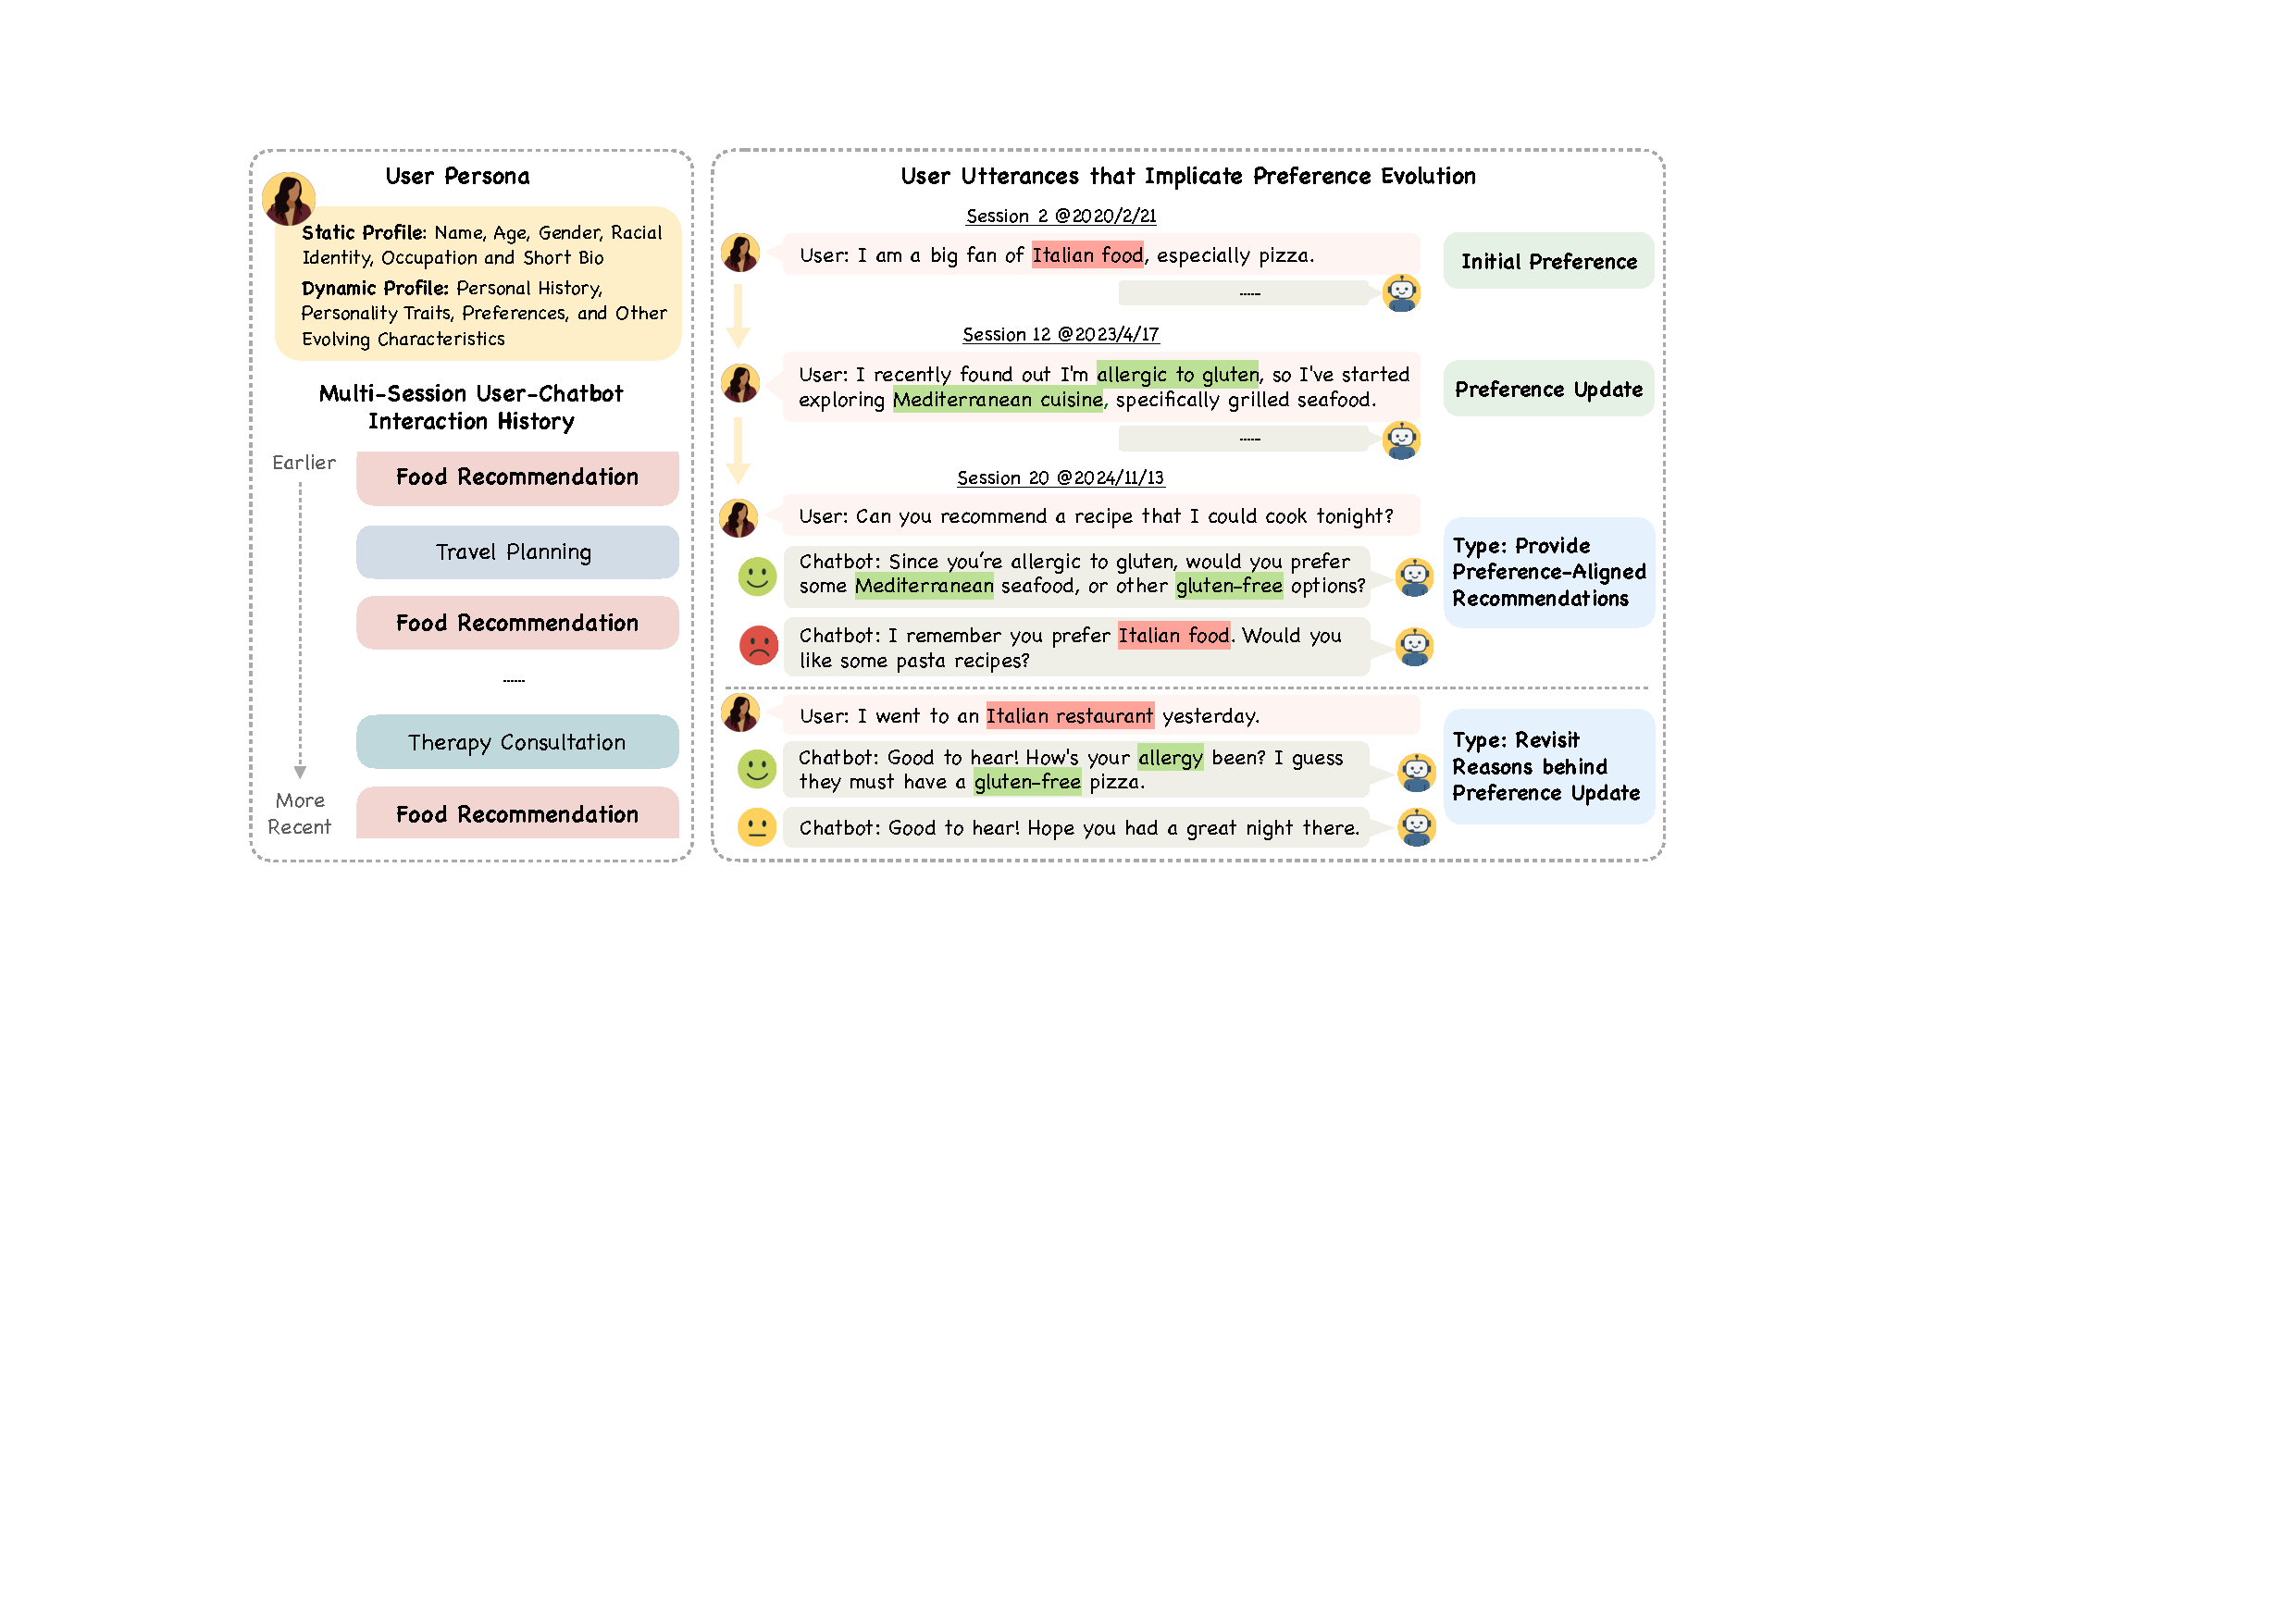
\includegraphics[width=1\linewidth]{figures/bench_overview.pdf}
  \caption{Overview of \datasetname~benchmark. Each benchmark sample is a user persona with static (e.g., demographic info.) and dynamic attributes (e.g., evolving preferences). Users engage with a chatbot in multi-session interactions across a variety of topics such as food recommendation, travel planning, and therapy consultation. As the user's preferences evolve over time, the benchmark offers annotated questions assessing whether models can track and incorporate the changes into their responses.}
  \vspace{-5mm}
  \label{fig:overview}
\end{figure}

%%% Original
% With \datasetnameemoji, we evaluate the ability of state-of-the-art LLMs to infer a user profile and how it evolves over time, as well as whether LLMs can apply what they learn about the user to provide personalized responses in different task scenarios. For this purpose, we design 7 types of \textit{in-situ} user requests (as shown in \autoref{tab:qa_types}), where the user issues new requests to LLM in a new conversation session from the first-person perspective. We evaluate if LLM is able to select the correct response that is aligned with the user's current state among distractor options. Overall, we observe that current LLMs still struggle to provide personalized responses based on the user's profile, with the frontier models such as GPT-4.5, o1, or Gemini-2.0-Flash scoring only around $50\%$ accuracy. 
% While models are typically performing reasonably well on recalling simple facts from the users and recognizing changes in users' preferences (with $60$-$70\%$ accuracy across models), they often struggle on acknowledging users' current situations, and delivering personalized responses accordingly (with $30$-$50\%$ accuracy). We provide detailed analysis on the factors that may impact model performance, such as the length of the interaction history, position in which the user preference is first/last mentioned, as well as the effect of having a separate retrieval component for memory recall, etc.  

With \datasetnameemoji, we evaluate whether state-of-the-art LLMs can infer evolving user profiles and generate personalized responses across task scenarios. To emulate the realistic settings in user-LLM interactions, we design 7 types of \textit{in-situ} user queries (\autoref{tab:qa_types}), where users issue queries to LLMs from first-person perspectives. We evaluate whether LLMs can select the correct response that best aligns with the current state of the user. We find that frontier models such as GPT-4.1, o4-mini, GPT-4.5, o1, or Gemini-2.0-Flash score only around $50\%$ overall accuracy and Llama-4-Maverick slightly lower at $43\%$ using direct prompt approaches.
While models perform reasonably well on recalling facts and tracking preference changes (60–70\% accuracy), they struggle to incorporate users’ latest situations into responses (30–50\% accuracy). We provide detailed analysis on how factors such as history length, preference positioning, and memory components may impact performance.

% We observe that current LLMs still struggle to recognize the dynamic evolution in users' profiles over time through direct prompt approaches.
% As a consequence,  LLMs often fail to deliver responses that align with users' current situations and preferences. We hope that \datasetname, along with our proposed user profile and conversation simulation pipeline can facilitate future research in the development of truly user-aware chatbots.

To summarize our key contributions and findings:
\begin{itemize}[itemsep=2pt, left=0pt]
\vspace{-2mm}
\item We propose the \datasetnameemoji~benchmark and its synthetic dialog generation pipeline for persona-oriented, multi-session, and timelined user-chatbot interaction history. 
% to evaluate LLMs capability to deliver personalized response across 15 task scenarios. 
% Our benchmark concerns realistic user-centric settings. We ground data generation on diverse user personas, closely reflecting real-world conversation scenarios that require personalization capabilities.
\item We assess 15 LLMs on 7 types of \textit{in-situ} user queries and evaluate their ability to provide responses aligned with user's dynamically changing profile across 15 task scenarios.    
% We develop a cost-effective, flexible, and scalable approach for generating synthetic conversation data tailored to multi-turn user-model interactions.
% \vspace{2mm}
\item With \datasetname, we observe that frontier models such as GPT4.1, o4-mini, GPT-4.5, o1, DeepSeek-R1, Gemini-2.0, Llama-4, and Claude-3.7 still struggle to be user-aware and deliver personalized responses, especially when the knowledge of the user needs to be applied across new scenarios. 
% with the biggest challenge in delivering personalized responses in new scenarios.
% responses according to user's latest preference and situation, and reason over users' profiles across different task scenarios.  
% Frontier models such GPT-4.5 and Gemini-1.5 achieve the highest personalization performance but still hover around only 52\% accuracy in multiple-choice settings, while reasoning models such as o1, o3-mini, and DeepSeek-R1 also struggle with the task. Generalization to new scenarios remains the greatest challenge in personalization.
% \item 
\end{itemize}
% in order for our data to achieve this goal. what data look like: simulated user profile and across different scenarios (list all), interact over time-->reflect their changes of xxx and be draw from session interaction.

% In practice, however, a practical difficulty comes from the fact that LLMs do not readily have access to all information about an user.  

% they are increasingly being deployed as personalized assistants, offering recommendations, consultations, and context-aware responses that adapt to individual user needs.

% Many users today rely on LLMs as their \textit{personalized} chatbots for a wide range of tasks. They harness these models’ assistance in everything from everyday planning to specialized problem-solving [TODO: add scenarios from papers].
% As these models become ever more ubiquitous in daily workflows, their ability to adapt to individual user profiles and preferences has grown in significance for enhancing user satisfaction and trust. Yet, achieving robust personalization at scale introduces several challenges, including accurately representing user profiles derived from extensive conversational histories and effectively tracking their continuous evolution over time. 

% For example, as illustrated in Figure\ref{fig:overview}, a user previously interacting with an LLM chatbot for food recommendations explicitly stated, "Following classic recipes is a better choice than experimenting with fusions," and elaborated her reasoning. Even after moving on to other unrelated tasks, the user's subsequent interactions continue to expand her historical profile. Therefore, the next time she seeks food recommendations, a well-personalized LLM should align its suggestions with the user's established preference for traditional cuisine or acknowledge her perspective explicitly. In contrast, poorly personalized responses might inaccurately recall user preferences or fail to capture the evolving nature of her interests over time [TODO: give examples of out incorrect answers]. Such challenges highlight the critical need for systematic benchmarking to ensure LLMs consistently "know" users deeply and "respond" effectively throughout ongoing interactions.

% In this work, we introduce the \datasetname~ benchmark to assess personalization performance across three key aspects:
% [TODO: callout our three questions]
% \begin{enumerate}
%     \item Can LLMs accurately learn about users' inherent traits and preferences from extensive interaction histories?
%     \item Can LLMs effectively track and recognize how users' preferences and situations evolve over time?
%     \item  Can LLMs use what it knows about the user to adapt their responses accordingly?
% \end{enumerate}


% Memory is a fundamental capability for enabling Large Language Models (LLMs) to act as agents~\citep{kapoor2024ai, jiang2024towards, durante2024agent}, capable of adapting to diverse user personas~\citep{ge2024scaling} and preferences in dynamic, interactive, and conversational scenarios. By maintaining a good memory of prior interactions, a model can develop long-term, personalized engagements with user's preferences, background, and context. Without a memory, it could make responses that merely make sense in general, or fail to adapt effectively to each user's unique needs. Therefore, proper handling of memory serves as a cornerstone towards personalization~\citep{chen2024persona, zhang2024personalization, chen2024large}, allowing LLMs to tailor their outputs based on previous interactions with users, enhancing user satisfaction.

% Although numerous research advances have been made to enhance and investigate the memorization capabilities of LLMs, a comprehensive benchmark suite that rigorously evaluates their \textit{memory recall in personalized scenarios} is still lacking. Most existing memory benchmarks are constrained only to contrived, relatively simple factual recall tasks \cite{liu2024lost}, lacking the complex user personas and long-term contextual nuances essential for genuinely personalized interactions \citep{maharana2024evaluating, wu2024longmemeval}.
% % TODO: tencent

% Unlike existing long-term memory benchmarks, we aim to evaluate whether LLMs can recall user personas and preferences over prolonged user-agent conversations, moving beyond static knowledge to dynamic updates across sessions at different times. We also present fine-grained challenges to assess how effectively the model can utilize its memory about the user to generate personalized content and recommendations in diverse application scenarios.
% To summarize our contributions:
% \begin{itemize}[noitemsep]
% \item Our benchmark concerns realistic user-centric settings. We ground data generation on diverse user personas, closely reflecting real-world conversation scenarios that require memory capabilities.
% \item We extend the evaluation of memorization to personalized generation, utilizing memory to generate persona-oriented conversations across diverse topics.
% \item We develop a cost-effective, flexible, and scalable approach for generating synthetic conversation data tailored to long, multi-turn, and multi-session user-model interactions.
% \end{itemize}

% TODO: One of the contributions is to simulate realistic scenarios of users using AI models as assistants. We can define what realistic means in our work. 



\section{\datasetnameemoji~Benchmark: Overview}\label{sec:overview}
We present an overview of the \datasetname~benchmark in Figure \ref{fig:overview}. 
Each instance in the benchmark dataset features a \textit{user profile or persona}, which includes basic demographic information (such as name, age, gender, and occupation), as well as \textit{dynamic} user characteristics such as user traits, preferences, and events happening in the user's life.  The dynamic user characteristics change over time as different events happen to the user that will lead to changes in users' traits and preferences specific to each task scenario. 

At different points in time of a user's profile evolution, the user engages in multi-turn conversations with LLM and seeks help or suggestions from LLM on one of the task scenarios. In each task scenario, the user would ask for the LLM's suggestions given the user's need and current situation. The conversation sessions across different tasks are interleaved by the temporal order in which the sessions happen.

To understand how well LLM chatbots can track the evolution in a user's profile from the conversation histories, we evaluate LLMs by whether they can provide the most suitable response to \emph{in-situ} user queries, where the user issues the query to LLM in a new conversation session from the first-person perspective. Depending on the time of the \emph{in-situ} query, the expected response from the model will differ. We cast the problem as a multiple-choice selection, where LLM needs to identify the correct response out of four choices, where the incorrect choices are based on either outdated or irrelevant information with respect to the current state of the user's profile. 

\paragraph{Types of skills evaluated.}
To evaluate LLMs' ability to (1) memorize the user profile, (2) track how the user profile evolve over time, and (3) generate personalized responses accordingly in new scenarios, we design the following 7 types of \emph{in-situ} user queries in the \datasetname~benchmark. We include examples for each type of user queries in \autoref{tab:qa_types}. 

\begin{enumerate}[left=0pt, itemsep=2pt]
    \item \textbf{Recall user-shared facts.} We evaluate whether a personalized chatbot can recall static events, activities, or interests the user has shared in previous interactions, and incorporate the information in its responses.
    \item \textbf{Suggest new ideas.} We evaluate whether a chatbot can suggest new items or activities that have not been mentioned in the interaction history, when users explicitly request so, e.g. ``\textit{suggest new restaurants I haven't ordered from before}''.
    \item \textbf{Acknowledge latest user preferences.} We evaluate whether a chatbot can recognize the latest preference expressed by the user in the interaction history.
    \item \textbf{Track full preference evolution.} We evaluate whether a chatbot can keep track of how users' preferences shift by time.
    \item \textbf{Revisit reasons behind preference updates.} We evaluate whether a chatbot can recall the reason(s) or event(s) leading to the preference change from a user.  
    \item \textbf{Provide preference-aligned recommendations.} We test whether a chatbot can proactively offer new recommendations
    that aligns with the user's current preferences.
    \item \textbf{Generalize to new scenarios.} We evaluate whether a chatbot can transfer what it learns about the user from other task scenarios to a new task.  
\end{enumerate}

\paragraph{Benchmark data statistics.}
\datasetnameemoji~features 20 personas, with over 180 interaction histories. Each interaction history contains 10, 20, or 60 sessions, where we dynamically adjust the total length of the history to approximately 32$k$, 128$k$, and 1$M$ tokens, respectively. Each session consists of 15–30 conversation turns between a user and an LLM chatbot. The user-LLM conversations span across 15 diverse topics, ranging from therapy and legal advice to recommendations on books, music, movies, and food; personal matters such as family, dating, health, and finance; and practical tasks like travel planning, online shopping, studying tips, and home decoration. In total, the benchmark features around 6$k$ \emph{in-situ} user query and LLM response pairs across the 7 query types. Detailed dataset breakdown is discussed in Appendix~\ref{app:breakdown}. The size of our benchmark is not limited by the scalability of the synthetic data pipeline but to make the evaluation cost reasonable.

% these configurations are not the upper limit of our benchmark's scalability, but are chosen for evaluation efficiency and limited by the maximum context window of current LLMs.
\begin{table}[htbp]
\centering \normalsize
\resizebox{0.9\textwidth}{!}{%
\begin{tabular}{p{0.22\linewidth} p{0.72\linewidth}}
\toprule
\textbf{Query type} & \textbf{Examples of \textit{in-situ} user queries and chatbot responses} \\
\midrule
\textbfblue{[1] Recall user-shared facts} & \textit{"User: I shared my \raisebox{0pt}[0.8\height][0.8\depth]{\setlength{\fboxsep}{0pt}\colorbox[rgb]{0.737,0.890,0.580}{\strut playlist}} with my friends and they loved it. ...... (later) User: What are some creative ways to share music? --- Chatbot: Curating personalized {\setlength{\fboxsep}{0pt}\colorbox[rgb]{0.737,0.890,0.580}{\strut playlists}} can be fun."}\\
\midrule
\textbfblue{[2] Suggest new ideas} & \textit{"User: ...... (later) User: Suggest new restaurant I {\setlength{\fboxsep}{0pt}\colorbox[rgb]{0.737,0.890,0.580}{\strut haven't}} ordered before."} \\
\midrule
\textbfblue{[3] Acknowledge latest user preferences} & \textit{"User: I am a big fan of {\setlength{\fboxsep}{0pt}\colorbox[rgb]{1.000,0.639,0.608}{\strut Italian}} food. ...... (later) User: I prefer {\setlength{\fboxsep}{0pt}\colorbox[rgb]{0.737,0.890,0.580}{\strut Mediterranean}} cuisine now. ... (later) User: I went to an Italian restaurant yesterday --- Chatbot: Nice to hear! Though I thought you prefer {\setlength{\fboxsep}{0pt}\colorbox[rgb]{0.737,0.890,0.580}{\strut Mediterranean}} food now."} \\
\midrule
\textbfblue{[4] Track full preference evolution} & \textit{"User: ...... (later) User: I am thinking about attending a cooking class. --- Chatbot: I understand your perspective on cooking classes has evolved. Initially, you expressed a {\setlength{\fboxsep}{0pt}\colorbox[rgb]{1.000,0.639,0.608}{\strut dislike}}, but later you mentioned your {\setlength{\fboxsep}{0pt}\colorbox[rgb]{0.737,0.890,0.580}{\strut interest}} in them."} \\
\midrule
\textbfblue{[5] Revisit reasons behind preference updates} & \textit{"User: I am a big fan of Italian food. ...... (later) User: I recently found I'm {\setlength{\fboxsep}{0pt}\colorbox[rgb]{0.737,0.890,0.580}{\strut allergic to gluten}}, so I've shifted to other dishes. ... (later) User: I went to an Italian restaurant yesterday --- Chatbot: How's your {\setlength{\fboxsep}{0pt}\colorbox[rgb]{0.737,0.890,0.580}{\strut allergy}} been? I guess they must have a {\setlength{\fboxsep}{0pt}\colorbox[rgb]{0.737,0.890,0.580}{\strut gluten-free}} pizza."} \\
\midrule
\textbfblue{[6] Provide preference aligned recommendations} & \textit{User: I prefer {\setlength{\fboxsep}{0pt}\colorbox[rgb]{0.737,0.890,0.580}{\strut Mediterranean}} seafood now. ...... (later) User: How can I make impactful lifestyle changes? --- Chatbot: How about diving into the {\setlength{\fboxsep}{0pt}\colorbox[rgb]{0.737,0.890,0.580}{\strut Mediterranean}} diet plan?"} \\
\midrule
\textbfblue{[7] Generalize to new scenarios} & \textit{"User: I prefer my yoga class because of its {\setlength{\fboxsep}{0pt}\colorbox[rgb]{0.737,0.890,0.580}{fixed weekly schedule}}. ...... (later) User: I recently haven’t had time to cook. --- Chatbot: Since you seem to love {\setlength{\fboxsep}{0pt}\colorbox[rgb]{0.737,0.890,0.580}{routine}} would you be interested in weekly scheduled bento-box deliveries?"} \\
\bottomrule
\end{tabular}
}
\caption{Examples of the 7 types of \emph{in-situ} user queries and expected chatbot response in the \datasetnameemoji~benchmark. We highlight words that signal the user's facts or preferences.}
\label{tab:qa_types}
\vspace{-2mm}
\end{table}


% \subsection{Design Principles and Challenges}
% We present an overview of our benchmark in Figure \ref{fig:overview}. The \datasetname~ benchmark suite consists of two key components: (1) a collection of tasks designed to embody personalization challenges through user-chatbot interactions. (2) a scalable pipeline for generating large-scale persona-oriented multi-session conversations ([TODO: add ref to 3.2]). 

% As illustrated in Figure \ref{fig:overview}, our comprehensive interaction history between users and LLM chatbots contains static user profile information, such as demographic and professional details. Additionally, these conversations capture dynamic user traits and preferences, tracking their evolution over time. This design equips LLM chatbots with rich contextual information, enabling them to dynamically profile users.

% To evaluate the capability of LLM chatbots in utilizing the aforementioned conversation histories to generate personalized responses, we propose a series of fine-grained personalization challenges and assess chatbot performance on these tasks. Figure \ref{fig:overview} demonstrates one example of evaluating the ability of LLM chatbots to generate personalized \textit{recommendations} aligned with users' evolving preferences. Furthermore, we create additional task types that probe the LLMs' abilities to recognize and understand the evolution of user information and the underlying reasons driving these changes. Additionally, we examine whether LLMs can integrate this user knowledge effectively to provide personalized responses and generalize this understanding to novel scenarios. We posit that a truly personalized LLM chatbot should proficiently exhibit these capabilities.

% \subsection{Multi-Session Conversation Data Overview}
% We define a \textit{session} as consecutive multi-turn conversations within a specific time frame. \datasetname\ features synthetic multi-session user-chatbot interactions \textit{centered around user personas}, minimizing irrelevant or randomly injected context. 
% It includes over 180 interaction histories and 20 personas, each constructed with 10, 20, or 60 conversation sessions—corresponding to approximately 32$k$, 128$k$, and 1$M$ tokens, respectively, and around 6$k$ question-answer pairs in total. Each context involves a single user. These configurations are not the upper limit of our benchmark's scalability, but are chosen for evaluation efficiency and limited by the maximum context window of current LLMs.

% We cover 15 diverse topics, ranging from therapy and legal advice to recommendations on books, music, movies, and food; personal matters such as family, dating, health, and finance; and practical tasks like travel planning, online shopping, studying tips, and home decoration. Each session consists of 15–30 rounds of user-model interactions.
% % creative writing, email composition, and code programming. 

% % Each topic comprises multiple conversation sessions arranged chronologically, with around 20 events per session. Each event includes a timestamp and may involve preference updates occurring across sessions under the same topic. Each session consists of 15–30 rounds of user-model interactions.

% % \datasetname\ includes over 180 interaction histories and 20 personas, each constructed with 10, 20, or 60 conversation sessions—corresponding to approximately 32$k$, 128$k$, and 1$M$ tokens, respectively, and around 6$k$ question-answer pairs in total. These configurations are not the upper limit of our benchmark's scalability, but are chosen for evaluation efficiency and limited by the maximum context window of current LLMs.


% Unlike questions framed from a third-person perspective, \datasetname\ simulates a more realistic scenario in which each question is posed directly by the user during multi-turn interactions. During evaluation, the model receives the relevant context available at the cutoff point where the user asks a question or sends a message and expects a model response.


% Each session contains approximately 20 events related to the topic and marked with their timestamps, with some events shared across sessions under the same topic, reflecting changes in user preferences over time. The development of these events throughout the user-model conversations forms event sequences, which serve as memory points for evaluation. 
% For conversational data under each persona, different topics are independent of one another, except for their shared seeding persona. Sessions range from TODO to TODO interaction rounds, with each round consisting of TODO to TODO sentences. The total context length of TODO–TODO($>$ 400k) tokens.


% This benchmark consists of synthetic multi-turn and multi-session conversation data, each centered around a unique persona expanded from the samples in \personahub~\citep{ge2024scaling}. Each conversation session takes place between a single user and the model, and we include TODO distinct personas.

% We cover 10 conversation topics, including therapy consultation, legal consultation, dating consultation, food recommendation, study consultation, travel planning, online shopping, creative writing, email writing, and code programming. Among these, creative writing, email writing, and code programming consist of single-session conversations, while the other topics span four conversation sessions occurring at different time points: from about 10 years ago to the present, from now to next week, from next week to next month, and from next month to next year.

% Each session contains approximately TODO–TODO(Around 20) events related to the topic and marked with their timestamps, with some events shared across sessions under the same topic, reflecting changes in user preferences over time. The development of these events throughout the user-model conversations forms event sequences, which serve as memory points for evaluation. 
% For conversational data under each persona, different topics are independent of one another, except for their shared seeding persona. Sessions range from TODO to TODO interaction rounds, with each round consisting of TODO to TODO sentences. The total context length of TODO–TODO($>$ 400k) tokens.


% \subsection{Overview of the Question Answering Tasks}
% \subsection{Evaluating Personalized Generation: Challenges}
% \subsection{Evaluating Personalized Generation: Tasks}
% \label{sec:tasks}
% Personalization is a fine-grained task that requires the model to generate responses tailored to each specific user, leveraging the memory and understanding of user profiling from user-model interactions, rather than merely providing a generally correct response. We identify seven fine-grained but important challenges included in \datasetname.
% Therefore, \datasetname\ presents the following question-answering tasks at varying levels of granularity, each of which focuses on different detailed aspects of memory and personalization.



% \begin{enumerate}[label=\textbf{(\alph*)}]
%     \item \textbf{Internalize the user’s inherent traits and preferences.} Sec.%~\ref{sec:challenge1}
%     \begin{enumerate}
%         \item[(a.1)] Incorporating User-Shared Facts. 
%     \end{enumerate}
    
%     \item \textbf{Track how the user profiling and preference evolve over time.} %Sec.~\ref{sec:challenge2}
%     \begin{enumerate}
%         \item[(b.1)] Acknowledging Latest Preferences.
%         \item[(b.2)] Tracking Full Preference Evolution.
%         \item[(a.3)] Revisiting Reasons behind Preferences.
%     \end{enumerate}

%     \item \textbf{Generate personalized responses accordingly in new scenarios.} %Sec.~\ref{sec:challenge3}
%     \begin{enumerate}
%         \item[(c.1)] Identifying New Facts Not Shared Before. 
%         \item[(c.2)] Generalizing Reason to New Scenarios.
%         \item[(c.3)] Preference-Aligned Recommendations.
%     \end{enumerate}
% \end{enumerate}


% \begin{enumerate}[label=\textbf{(\alph*)}]
%     \item \textbf{Personalizing with User-Shared Facts} Sec.~\ref{sec:challenge1}
%     \begin{enumerate}
%         \item[(a.1)] Incorporating User-Shared Facts. %\textit{Fact Incorporation:} Incorporating facts previously shared by the user.
%         \item[(a.2)] Identifying New Facts Not Shared Before. % \textit{Novel Facts:} Identifying new things not mentioned by the user.
%     \end{enumerate}
    
%     \item \textbf{Personalizing with User Preferences} Sec.~\ref{sec:challenge2}
%     \begin{enumerate}
%         \item[(b.1)] Incorporating Latest Preference. %\textit{Latest Preference:} Adapting to the latest user preferences.
%         \item[(b.2)] Tracking Full Preference Evolution.  % \textit{Full Evolution:} Tracking the full evolution of preference updates.
%     \end{enumerate}

%     \item \textbf{Understanding Reasons behind Preference Updates} Sec.~\ref{sec:challenge3}
%     \begin{enumerate}
%         \item[(c.1)] Revisiting Previous Reasons. %\textit{Reason Recall:} Revisiting reasons behind previous updates.
%         \item[(c.2)] Generalizing Reason to New Scenarios. %\textit{Reason Generalization:} Generalizing past reasons to new scenarios.
%     \end{enumerate}
    
%     \item \textbf{Providing Personalized Recommendations} Sec.~\ref{sec:challenge4}
%     \begin{enumerate}
%         \item[(d.1)] Preference-Aligned Recommendations. %\textit{Recommendations:} Crafting recommendations aligned with latest preferences.
%         % \item[(d.2)] Crafting new samples aligned with the user’s style.
%     \end{enumerate}
% \end{enumerate}




% \begin{table}[t]
% \centering
% \begin{tabularx}{\textwidth}{ll}
% \toprule
% \textbf{Detailed Question Type} & \textbf{Research Question(s)} \\
% \midrule
% \textbf{(a.1) Incorporate shared facts} & RQ1: Internalize user traits \\
% \multicolumn{2}{p{\dimexpr\textwidth-2\tabcolsep\relax}}{\textbf{Example Question:} "Suggest engaging activities for a fun-filled game night."} \\
% \multicolumn{2}{p{\dimexpr\textwidth-2\tabcolsep\relax}}{\textbf{Example Answer(s):} Correct Answer: "Based on your interest in board games, I suggest a themed board game night with friends." --- Incorrect Answer: "I recommend a solo crossword puzzle."} \\
% % \multicolumn{2}{p{\dimexpr\textwidth-2\tabcolsep\relax}}{\textbf{Explanation:} Incorporate shared facts from previous interactions (e.g., user’s favorite activities) to tailor responses that feel personally relevant.} \\
% \midrule
% \textbf{(a.2) Identify new facts} & RQ1: Internalize user traits \\
% \multicolumn{2}{p{\dimexpr\textwidth-2\tabcolsep\relax}}{\textbf{Example Question:} "Suggest a new restaurant I haven’t tried."} \\
% \multicolumn{2}{p{\dimexpr\textwidth-2\tabcolsep\relax}}{\textbf{Example Answer(s):} Correct Answer: "Since you enjoyed Italian food before, consider trying the new Japanese restaurant downtown." --- Incorrect Answer: "You should revisit that same Italian restaurant."} \\
% % \multicolumn{2}{p{\dimexpr\textwidth-2\tabcolsep\relax}}{\textbf{Explanation:} Identify and integrate new, unmentioned facts to avoid repetition and promote novelty in recommendations.} \\
% \midrule
% \textbf{(b.1) Incorporate latest preference} & RQ2: Track evolving preferences \\
% \multicolumn{2}{p{\dimexpr\textwidth-2\tabcolsep\relax}}{\textbf{Example Question:} "I saw a cultural festival in town yesterday."} \\
% \multicolumn{2}{p{\dimexpr\textwidth-2\tabcolsep\relax}}{\textbf{Example Answer(s):} Correct Answer: "It sounds like you enjoyed the festival; perhaps you would also appreciate the upcoming art exhibit with similar themes." --- Incorrect Answer: "Maybe you should try a sports event next time."} \\
% % \multicolumn{2}{p{\dimexpr\textwidth-2\tabcolsep\relax}}{\textbf{Explanation:} Leverage the user’s most recent expressed preferences to generate contextually updated responses.} \\
% \midrule
% \textbf{(b.2) Track full evolution} & RQ2: Track evolving preferences \\
% \multicolumn{2}{p{\dimexpr\textwidth-2\tabcolsep\relax}}{\textbf{Example Question:} (Example omitted)} \\
% \multicolumn{2}{p{\dimexpr\textwidth-2\tabcolsep\relax}}{\textbf{Example Answer(s):} Correct Answer: "Considering your journey from quiet cafes to lively concerts, I recommend an eclectic music café that blends both atmospheres." --- Incorrect Answer: "I suggest a generic fast food chain."} \\
% % \multicolumn{2}{p{\dimexpr\textwidth-2\tabcolsep\relax}}{\textbf{Explanation:} Track how user preferences shift across interactions, ensuring consistency over time.} \\
% \midrule
% \textbf{(c.1) Revisit previous reasons} & RQ2 \& RQ3: Track evolution \& generate responses \\
% \multicolumn{2}{p{\dimexpr\textwidth-2\tabcolsep\relax}}{\textbf{Example Question:} "Did you change your stance on authentic flavor?"} \\
% \multicolumn{2}{p{\dimexpr\textwidth-2\tabcolsep\relax}}{\textbf{Example Answer(s):} Correct Answer: "Yes, after mentioning your positive experience at the classic bistro, it seems your preference has shifted towards traditional flavors." --- Incorrect Answer: "No, your taste appears inconsistent."} \\
% % \multicolumn{2}{p{\dimexpr\textwidth-2\tabcolsep\relax}}{\textbf{Explanation:} Revisit earlier justifications for preference changes to ground follow-up suggestions or inquiries.} \\
% \midrule
% \textbf{(c.2) Generalize reasons} & RQ2 \& RQ3: Track evolution \& generate responses \\
% \multicolumn{2}{p{\dimexpr\textwidth-2\tabcolsep\relax}}{\textbf{Example Question:} (Example omitted)} \\
% \multicolumn{2}{p{\dimexpr\textwidth-2\tabcolsep\relax}}{\textbf{Example Answer(s):} Correct Answer: "Given your preference for routines due to a busy schedule, a weekly meal kit service might suit your needs." --- Incorrect Answer: "Maybe try something random like an all-you-can-eat buffet."} \\
% % \multicolumn{2}{p{\dimexpr\textwidth-2\tabcolsep\relax}}{\textbf{Explanation:} Generalize previously stated reasoning to new, related scenarios or decisions.} \\
% \midrule
% \textbf{(d.1) Provide recommendations} & RQ3: Generate personalized responses \\
% \multicolumn{2}{p{\dimexpr\textwidth-2\tabcolsep\relax}}{\textbf{Example Question:} "Suggest a new restaurant I haven’t tried before."} \\
% \multicolumn{2}{p{\dimexpr\textwidth-2\tabcolsep\relax}}{\textbf{Example Answer(s):} Correct Answer: "I recommend the new fusion restaurant downtown, which aligns with your evolving taste for innovative cuisines." --- Incorrect Answer: "How about the old chain restaurant you always visit?"} \\
% % \multicolumn{2}{p{\dimexpr\textwidth-2\tabcolsep\relax}}{\textbf{Explanation:} Offer proactive suggestions aligned with the evolving user profile, anticipating user needs even when not restated.} \\
% \bottomrule
% \end{tabularx}
% \caption{TODO}
% \label{tab:qa_types}
% \end{table}


% \begingroup
% \setstretch{1.2}
% \begin{table}[t]
% \centering
% \small
% \begin{tabularx}{\textwidth}{X >{\raggedleft\arraybackslash}p{5cm}}
% \toprule
% \textbf{Question Types in \datasetname} & \textbf{Research Question(s)} \\
% \midrule
% \textbf{Static Information} \\
% \midrule
% \textbfblue{[1] Incorporate User-Shared Facts} & RQ1 \\
% \multicolumn{2}{p{\dimexpr\textwidth-2\tabcolsep}}{\textbf{Explanation:} A personalized chatbot should be able to internalize static events, activities, or interests the user has shared in previous interactions in its responses.} \\
% \multicolumn{2}{p{\dimexpr\textwidth-2\tabcolsep}}{\textbf{Example} \textit{"User: I shared my \raisebox{0pt}[0.8\height][0.8\depth]{\setlength{\fboxsep}{0pt}\colorbox[rgb]{0.737,0.890,0.580}{\strut playlist}} with my friends and they loved it. ...... (later) User: What are some creative ways to share music? --- Chatbot: Curating personalized {\setlength{\fboxsep}{0pt}\colorbox[rgb]{0.737,0.890,0.580}{\strut playlists}} can be fun."}} \\
% \midrule
% \textbfblue{[2] Identify New Facts Not Shared Before} & RQ1 \& RQ3 \\
% \multicolumn{2}{p{\dimexpr\textwidth-2\tabcolsep}}{\textbf{Explanation:} A personalized chatbot should be able to recall relevant details from its internal user-model interaction history and identity items or activities novel to the user.} \\
% \multicolumn{2}{p{\dimexpr\textwidth-2\tabcolsep}}{\textbf{Example} \textit{"User: ...... (later) User: Suggest new restaurant I {\setlength{\fboxsep}{0pt}\colorbox[rgb]{0.737,0.890,0.580}{\strut haven't}} ordered before.}} \\
% \midrule
% \textbf{Dynamic Information} \\
% \midrule
% \textbfblue{[3] Acknowledging Latest User Preferences} & RQ1 \& RQ2 \\
% \multicolumn{2}{p{\dimexpr\textwidth-2\tabcolsep}}{\textbf{Explanation:} A personalized chatbot should be able to internalize user preferences in its responses and understand the latest one from preference evolution over time} \\
% \multicolumn{2}{p{\dimexpr\textwidth-2\tabcolsep}}{\textbf{Example} \textit{"User: I am a big fan of {\setlength{\fboxsep}{0pt}\colorbox[rgb]{1.000,0.639,0.608}{\strut Italian}} food. ...... (later) User: I prefer {\setlength{\fboxsep}{0pt}\colorbox[rgb]{0.737,0.890,0.580}{\strut Mediterranean}} seafood now. ... (later) User: I went to an Italian restaurant yesterday --- Chatbot: Nice to hear! Though I thought you prefer {\setlength{\fboxsep}{0pt}\colorbox[rgb]{0.737,0.890,0.580}{\strut Mediterranean}} food now.}} \\
% \midrule
% \textbf{[4] Track Full Preference Evolution} & RQ1 \& RQ2 \\
% \multicolumn{2}{p{\dimexpr\textwidth-2\tabcolsep}}{\textbf{Explanation:} A personalized chatbot should be able to track how user preferences shift across interactions over time.} \\
% \multicolumn{2}{p{\dimexpr\textwidth-2\tabcolsep}}{\textbf{Example} \textit{"User: ...... (later) User: I am thinking about attending a cooking class. --- Chatbot: I understand your perspective on cooking classes has evolved. Initially, you expressed a {\setlength{\fboxsep}{0pt}\colorbox[rgb]{1.000,0.639,0.608}{\strut dislike}}, but later you mentioned a {\setlength{\fboxsep}{0pt}\colorbox[rgb]{0.737,0.890,0.580}{\strut preference}} for them.}} \\
% \midrule
% \textbf{Dynamic Information in New Scenarios} \\
% \midrule
% \textbfblue{[5] Revisit Reasons Behind Preference Updates} & RQ1, RQ2, \& RQ3 \\
% \multicolumn{2}{p{\dimexpr\textwidth-2\tabcolsep}}{\textbf{Explanation:} A personalized chatbot should be able to remember why a user's preferences changed and revisit those reasons if they shift again in new scenarios.} \\
% \multicolumn{2}{p{\dimexpr\textwidth-2\tabcolsep}}{\textbf{Example} \textit{"User: I am a big fan of Italian food. ...... (later) User: I recently found I'm {\setlength{\fboxsep}{0pt}\colorbox[rgb]{0.737,0.890,0.580}{\strut allergic to gluten}}, so I've shifted to other dishes. ... (later) User: I went to an Italian restaurant yesterday --- Chatbot: How's your {\setlength{\fboxsep}{0pt}\colorbox[rgb]{0.737,0.890,0.580}{\strut allergy}} been? I guess they must have a {\setlength{\fboxsep}{0pt}\colorbox[rgb]{0.737,0.890,0.580}{\strut gluten-free}} pizza.}} \\
% \midrule
% \textbfblue{[6] Provide Preference-Aligned Recommendations} & RQ1, RQ2, \& RQ3 \\
% \multicolumn{2}{p{\dimexpr\textwidth-2\tabcolsep}}{\textbf{Explanation:} A personalized chatbot should be able to proactively offer new recommendations that aligns with the user profiling and preferences.} \\
% \multicolumn{2}{p{\dimexpr\textwidth-2\tabcolsep}}{\textbf{Example} \textit{User: I prefer {\setlength{\fboxsep}{0pt}\colorbox[rgb]{0.737,0.890,0.580}{\strut Mediterranean}} seafood now. ...... (later) User: How can I make impactful lifestyle changes? --- Chatbot: How about diving into the {\setlength{\fboxsep}{0pt}\colorbox[rgb]{0.737,0.890,0.580}{\strut Mediterranean}} diet plan?}} \\
% \midrule
% \textbfblue{[7] Generalize Reasons to New Scenarios} & RQ1, RQ2, \& RQ3 \\
% \multicolumn{2}{p{\dimexpr\textwidth-2\tabcolsep}}{\textbf{Explanation:} A personalized chatbot should be able to generalize reasons behind preferences to new scenarios by identifying relevant patterns.} \\
% \multicolumn{2}{p{\dimexpr\textwidth-2\tabcolsep}}{\textbf{Example} \textit{"User: I prefer my yoga class because of its {\setlength{\fboxsep}{0pt}\colorbox[rgb]{0.737,0.890,0.580}{fixed weekly schedule}}. ...... (later) User: I recently haven’t had time to cook. --- Chatbot: Since you seem to love {\setlength{\fboxsep}{0pt}\colorbox[rgb]{0.737,0.890,0.580}{routine}} would you be interested in weekly scheduled bento-box deliveries?}} \\
% \bottomrule
% \end{tabularx}
% \caption{Description of the 7 question types in \datasetname. For each type, we provide an explanation of the personalization challenge it addresses, an example of its application, and the relevant research questions. The highlighted texts TODO}
% \label{tab:qa_types}
% \end{table}
% \endgroup




% At the time of each questioning, the model has access to the full conversation history \textit{up to} the moment the user asks that question, ensuring the causality of the context. The full benchmark includes TODO question-answer pairs, and the distance between each question and the relevant reference information needed to answer it within the whole context spans TODO-TODO sessions and TODO–TODO tokens.


% \subsubsection{Personalizing with User-Shared Facts}\label{sec:challenge1}
% \subsubsection{Incorporating User-Shared Facts} Personalization requires incorporating factual details the user has shared in previous interactions—such as their favorite cuisines, preferred travel destinations, or types of pets they own. 
% % In real-world scenarios, users often phrase their queries naturally and conversationally, without explicitly referencing prior interactions or speaking in the third person. 
% For instance, a user might ask, \textit{"What are some engaging activities you would suggest for a fun-filled game night with friends?"} 
% % rather than \textit{"Which activity does this user like to do with friends?"}. 
% A personalized model should respond according to the user's previously mentioned activities or interests. % whereas other responses may include activities irrelevant to the current user.

% \subsubsection{Revisiting Reasons behind Preferences} Every preference update is grounded in some reasons. A personalized model should not only track how a user's preferences evolve but also remember and understand the underlying motivations behind those changes. 
% For example, suppose a user previously shifted their preference toward more traditional cuisine, saying, \textit{"I realized that classic restaurant is a better choice now since it preserves the authentic flavor."} Later, they mention, \textit{"I went to a new Japanese-French fusion bar."} A personalized model could follow up by revisiting the previous reasons, \textit{"Nice to hear! Though I’m curious—did you change your stance on authentic flavor?"} 

% \subsubsection{Acknowledging Latest Preference} Beyond factual information itself, a personalized model should also understand the user's preferences toward them. For instance, when a user says, \textit{"I saw a cultural festival in town yesterday."} the model should be able to reference the user’s prior preference for cultural festivals to craft a personalized response—whether it’s \textit{"I know how much you love these cultural festivals,"} or \textit{"I remember you were not really enjoying these festivals before."} More importantly, user profiling and preferences are dynamic and can evolve over time. A personalized model should accurately follow the user’s most recent preferences to give responses, rather than outdated ones. 

% % Traditional factual questioning on memory typically prompt the model to recall information from a third-person perspective, such as asking, \textit{"Which activity does this user like?"} However, in real-world interactions, users may casually post queries that lack explicit reference to previous conversations. In such cases, a personalized model should inherently recognize relevant past events or details this user has shared before and leverage that memory to provide informed responses. In contrast, non-personalized answers may either still be generally accurate answers but fail to incorporate past facts the user has discussed in the past, or incorporate incorrect facts of this user.

% % As two sides of the same coin, this type of question-answering also involves mimicking a user’s natural way of exploring new ideas—asking for something new without explicitly restating past experiences. A personalized model should be capable of recalling relevant details from the user’s entire conversation history, acknowledging what this user has and hasn't told it before, and automatically generating novel suggestions for this specific user.

% % \subsubsection{Personalizing with User Preferences}\label{sec:challenge2}

% \subsubsection{Tracking Full Evolution} To further challenge a model's capabilities, we evaluate whether it can track the entire evolution of user preference throughout the interaction history.



% % Beyond recalling factual information such as past events, activities, or other details, a personalized model should also take into account the user’s preferences toward them. More importantly, user preferences may evolve over time across conversation sessions. As a result, when the user mentions again something they have discussed before, we evaluate whether a model can not only memorize past preferences but also adapt its memory to changes, ensuring that it accurately follows the user's most recent preferences, rather than failing to distinguish them from outdated ones. To push the model to its limits, we also test whether it can recall the full sequence of the user's preference changes in the entire context, rather than just the final state. In both cases, we require the model to demonstrate its memory of the user's preferences in its responses.

% % \subsubsection{Understanding Reasons behind Preference Updates}\label{sec:challenge3}

% \subsubsection{Identifying Facts Not Shared Before} As two sides of the same coin, the user can also seek new experiences without explicitly restating their past ones, such as \textit{"Suggest new restaurant I haven’t ordered before."} A personalized model should recall relevant details from the user’s interaction history, understand what the user has and hasn’t previously mentioned, and generate novel suggestions instead of repeating existing ones.


% \subsubsection{Generalizing Reason to New Scenarios} Understanding the reasons is valuable for models to handle new scenarios. When the user brings up something new, a personalized model should recognize underlying similarities with related preferences. For example, if a user previously expressed a preference for yoga classes due to their fixed weekly schedule, the model could generalize this reason to suggest weekly scheduled bento-box deliveries, anticipating that the user may value routine.

% % Every preference update has a reason, and our data curation pipeline ensures that the user has mentioned the reason somewhere within the overall conversation. A personalized model should not only track changes in preference but also memorize and understand the reasons behind those changes. 

% % Our benchmark evaluates two ways in which the model can leverage such memory. First, if the user revisits a previously discussed topic but expresses a change in preference once again, we test whether the model can correctly inquire about what happened to the original reason. Second, if the user briefly introduces something new while discussing reasons similar to a past reason, we assess whether the model can recognize the similarity, generalize its memorized reasons to new scenarios, and proactively discuss whether the user would like or dislike the new item or activity.

% % \subsubsection{Providing Personalized Recommendations}\label{sec:challenge4}
% \subsubsection{Preference-Aligned Recommendations} A personalized model should proactively offer new recommendations or content that aligns with the user's evolving profiling and preferences. In real-world interactions, users naturally won’t restate their identity or reiterate all previously discussed preferences each time they seek suggestions. Instead, the model must leverage accumulated knowledge from past interactions to anticipate needs and deliver preference-aligned recommendations. 

% Writing tasks often require a high degree of personalization, including creative writing, email composition, and code programming. Users may engage with the model to revise or refine pieces of writing or code and offer feedback. When the same user later requests a new email or Python function, a personalized model should adapt to this user’s preferred style, tone, and formatting automatically, while avoiding elements they’ve previously expressed dissatisfaction with to ensure a more seamless user experience.


% The generation tasks in this section refer to creating novel content for the user, requiring the model to have more advanced memory capabilities to accurately understand and reflect the user's persona and preferences. 

% We provide two types of tasks. Firstly, in real-world scenarios, when users seek suggestions or recommendations, they typically do not restate who they are or reiterate all their previously discussed preferences. The challenge for the model is to accurately retrieve relevant memories and provide personalized recommendations, rather than offering generic suggestions that may fail to engage the specific user or even contradict their inherent preferences. Meanwhile, if there is a history of preference updates, the recommendation must align with the user's most recent preferences. 
% Additionally, we also include stereotypical answers based on racial and gender identities as incorrect options in this recommendation task, which are irrelevant to the user's actual interaction history.

% Secondly, we find writing tasks often require a high degree of personalization, including creative writing, email writing, and code programming. Users may engage in discussions with the model to rewrite or refine pieces of writing or code, providing feedback on whether they like or dislike certain revisions the model suggests. Given this interaction history in memory, when the same user later on requests a new email or Python function, for example, a personalized model should adapt to the user’s preferred style and formatting while avoiding elements they dislike, ensuring a more seamless interaction.



% We employ multiple-choice questions in both discriminative and generative settings to evaluate the model’s performance. In the \textbf{discriminative setting}, the model is provided with the question, four answer options with (a), (b), (c), and (d), and the full multi-session conversation history up to where this question is asked as the context. The model is prompted to select the best option for the user. In the \textbf{generative setting}, the model receives the same inputs but is evaluated based on its conditional probability of generating each of the four options, respectively. This is done by autoregressively appending each token from an option to the model's output and collecting the corresponding logit probabilities. The final answer will be the one with the highest joint probability over all tokens in its answer. %(TODO: we might add some formulas here)


\section{Constructing Examples in \datasetnameemoji~At Scale}
\label{sec:curation}
We develop a modular data curation pipeline—powered by GPT-4o~\citep{hurst2024gpt}—to synthesize persona-oriented, multi-session user–model conversations with long context. The pipeline minimizes irrelevant or randomly injected content to better evaluate how effectively LLM chatbots address the challenges outlined in Section~\ref{sec:overview}, while ensuring cost-effectiveness and scalability: generating data for each persona on each conversation topic costs approximately \$2, independent of the context window length up to 1$M$ tokens.


% We develop a modular data curation pipeline—powered by GPT-4o~\citep{hurst2024gpt}—to synthesize high-quality, persona-oriented, and multi-session user–model conversations with long context, minimizing irrelevant or randomly injected context, in order to evaluate how well language models address the challenges outlined in Section~\ref{sec:overview}, while maintaining cost-effectiveness and scalability.

% \datasetname~ features synthetic multi-session user-chatbot interactions centered around user personas, minimizing irrelevant or randomly injected context


% Given a conversational session and its associated meta-data of events and facts, we then generate grounded questions.




% \begin{figure}[t]
%   \centering
%   \includegraphics[width=1\linewidth]{figures/concatenate.pdf}
%   \caption{TODO}
%   % \vspace{-3mm}
%   \label{fig:concatenate}
% \end{figure}



% To evaluate the language model's performance on tasks requiring persona-aligned information from long-memory conversation datasets, we introduce a high-quality, diverse, and scalable data curation pipeline. Our approach replicates real-world scenarios in which LLM agents must retain user memory and adapt to diverse personas and unique interaction histories. Unlike benchmarks that focus solely on simple facts presented in short paragraphs or on lengthy yet contexts lacking relevance, \datasetname\ ensures that every interaction is anchored to a specific user persona engaging with the agent on a defined topic while maintaining temporal coherence. The following sections detail our systematic and scalable approach to curate long conversational data.

% In this section, we introduce our data curation pipeline to curate high-quality, multi-turn, and multi-session conversational data, in order to evaluate how well langauge models can adddress the challenges discussed in Section~\ref{sec:overview}. 
% Unlike existing memory benchmarks that either focus solely on the accuracy of simple facts or adopt a needle-in-a-haystack approach by injecting key phrases into loosely connected long contexts, \datasetname\ ensures that every interaction is anchored to a specific user persona engaging with the model on a specific topic, while maintaining temporal coherence. TODO: We can talk about this in intro or related work

% Generating high-quality long-form conversational data from scratch remains challenging, 
% % especially if one wants to generate millions of tokens from scratch.
% To address this, we introduce a modularized data curation pipeline that first focuses on generating individual conversation sessions and concatenates them afterwards to a satisfactory length, enabling cost-effective and scalable long-context generation.

% designed to generate high-quality, multi-turn, and multi-session conversational data
% replicating real-world scenarios in which language models must retain memory of the users and adapt to diverse user personas.

\paragraph{Constructe user profile and persona.}
We sample a set of random personas from \personahub~\citep{ge2024scaling}, each comprising about one to three sentences, and augment them with additional demographic information and extended personal details. We also construct a timeline and populate it with events that align with the persona. These events serve as the \textit{general personal history}, such as education, career development, and life experiences, to provide a richer context. The prompts used in the process can be found in Appendix~\ref{app:prompts}.


% We begin by collecting a diverse set of user personas from \personahub~\citep{ge2024scaling} that offers a billion synthetic personas, each consisting of approximately one to three sentences. We then expand these personas with additional details, including age, racial and gender identities, occupations, educational backgrounds, and other relevant characteristics. We further prompt OpenAI's GPT-4o model to propose five hobbies this person likes and dislikes, respectively, as the initial user preferences.


% \subsection{Generate Topic-Specific Personal Histories}
Building on the persona and general personal history, we generate one additional \textit{topic-specific personal history} for each conversation topic. Under each topic, we define a set of initial preferences, ensuring no overlap across different topics. Each topic-specific history includes events, timestamps, associated preferences, potential updates to those preferences, and the underlying reasons for those changes. This approach ensures a coherent progression of user experiences while maintaining a strong connection to their personas.


The structured personal histories also facilitate the curation of question–answer pairs. We leverage short-form information within these histories to extract ground-truth user profiles and preferences at any specific time, ensuring that the correct answers are both event- and persona-grounded. In contrast, distractor options, while generally reasonable, either overlook the user’s persona or contradict it. Additionally, we exclude all questions that the model can answer correctly without seeing any contextual information from the benchmark.



% We prompt GPT-4o to expand the initial persona into two chronological personal histories: general and topic-specific. The general history captures broad life events like college graduation related to the persona, which will be shared across all conversation topics. Each conversation topic will have its own topic-specific personal history.

% % Along the temporal axis of each personal history, 
% We generate $10$ events within last 10 years this user might have experienced, including both short-term and long-term ones. Each event is timestamped and linked to one of the five likes or dislikes defined in the persona.
% We further extend this process to generate personal histories for three other time periods: from now to next week, next week to next month, and next month to next year. Each period may introduce events linked to new likes or dislikes mentioned in the persona, as well as events with preference changes from the previous period accompanied by detailed reasons for the change. This approach ensures a coherent progression of user experiences while maintaining a strong connection to their preferences. 

\paragraph{Simulate conversation sessions from user profile.}
We divide the timeline into multiple segments, resulting in segments of personal histories that follow a causal, chronological order. Each segment is then expanded into a full user–model conversation session, designed to cover all details of the corresponding topic-specific personal history segment, together with additional storytelling context as if the user is talking with a chatbot naturally. For example, under the therapy consultation topic, we frame the interaction as a user seeking guidance from an AI therapist. 

To enhance the quality of the conversations, we incorporate several tricks: (1) Before generating each user–model interaction turn, we prompt GPT-4o to first identify and cite the relevant event from the personal history. These citations serve as internal guidance and are not included in the final evaluation data. (2) Since GPT-4o may miss some events, leading to incomplete preference update sequences, we employ a self-reflection mechanism. We ask GPT-4o to review the generated conversation and identify any missing events from the personal history, ensuring better coverage and coherence across the interaction.

% During evaluation, the model will only have access to conversations, not personal histories.

% Writing and coding topics are not tied to personal histories. Instead, we prompt GPT-4o to infer each user's explicit style and formatting preferences from their persona, avoiding subjective ones. Using real-world samples, we query GPT-4o to rewrite each sample to reflect these personalized preferences. We then simulate a user interacting with an AI writing or coding assistant to convert each original sample to the persona-aligned one. In these dialogues, the user highlights specific sentences or code pieces they find unsatisfactory in terms of style or format, and the assistant offers targeted editing suggestions.


% Once we have detailed personal histories, we have the foundation for generating actual conversations. Under each topic, we generate four causally connected conversation sessions, spanning from \textit{about 10 years ago to the present, from now to next week, from next week to next month, and from next month to next year.} Specifically, we prompt GPT-4o to transform each detailed history into a multi-turn conversation under the current topic. For example, when simulating a therapy consultation, we frame the interaction as a user seeking guidance from an AI therapist, trying to discuss every single event from their general and therapy-specific history. When generating each utterance, we ask GPT-4o to first cite relevant personal histories, including the timestamps, as side notes. Note that during evaluation, these side notes will be hidden from the model being assessed. 
% using a single thread in the OpenAI's Assistant API for each topic.

% However, two potential issues remain: (1) the conversation that GPT-4o generated may not cover all events in the personal histories. This is crucial because, \textit{during evaluation, models will have access only to the conversations, not the personal histories.} These histories are solely used for curating conversation data and evaluation questions. As a result, if certain events are missing from the conversations, the model will have no way to answer questions curated from these events. (2) We still find that each conversation may not be long enough.
% \begin{itemize}
%     \item We mitigate the first issue by leveraging \textit{self-reflection}. By providing the model with the target personal histories with all timestamps, along with the generated conversation with side notes, we prompt it to self-check for any missing timestamps and if any, insert them by generating new utterances. We find this helps cover the majority of previously missing events.
%     \item We address the second issue by prompting GPT-4o-mini to expand each pair of user and model utterances to at least five sentences, adding irrelevant context and details without alterning original meaning or user preferneces. This approach extends the final conversation length by approximately five times.
    % \item We address the second issue by breaking the conversation into utterance groups, each consisting of a side note, the user's utterance, and the model's response for a single event—typically totaling three sentences. We send each utterance group to GPT-4o-mini, requesting it to expand each utterance to at least five sentences by adding irrelevant context and details while preserving the original meaning. This approach helps expand the final conversation length by approximately five times.
% \end{itemize}


% \subsection{Curating Conversation Data for Writing Topics with Special Steps}
% Writing topics are not based on personal histories; instead, we query GPT-4o to propose the user's explicit style and format preferences based on personas. Using real-world writing samples in creative writing, email composition, and code programming, we prompt GPT-4o again to rewrite each sample to align with the user's specific style and format preferences. Next, given both a general and a persona-aligned sample, we transform them into multi-turn conversations, simulating a scenario where the user consults an AI writing assistant to refine their original work. In these conversations, the user explicitly refers to a sentence from the original sample, complaining about style or format issues, and the assistant provides editing suggestions. Different from other topics, these topics consist of multiple independent sessions, each generated from separate original writing or coding samples.
\begin{figure}[t]
  \centering
  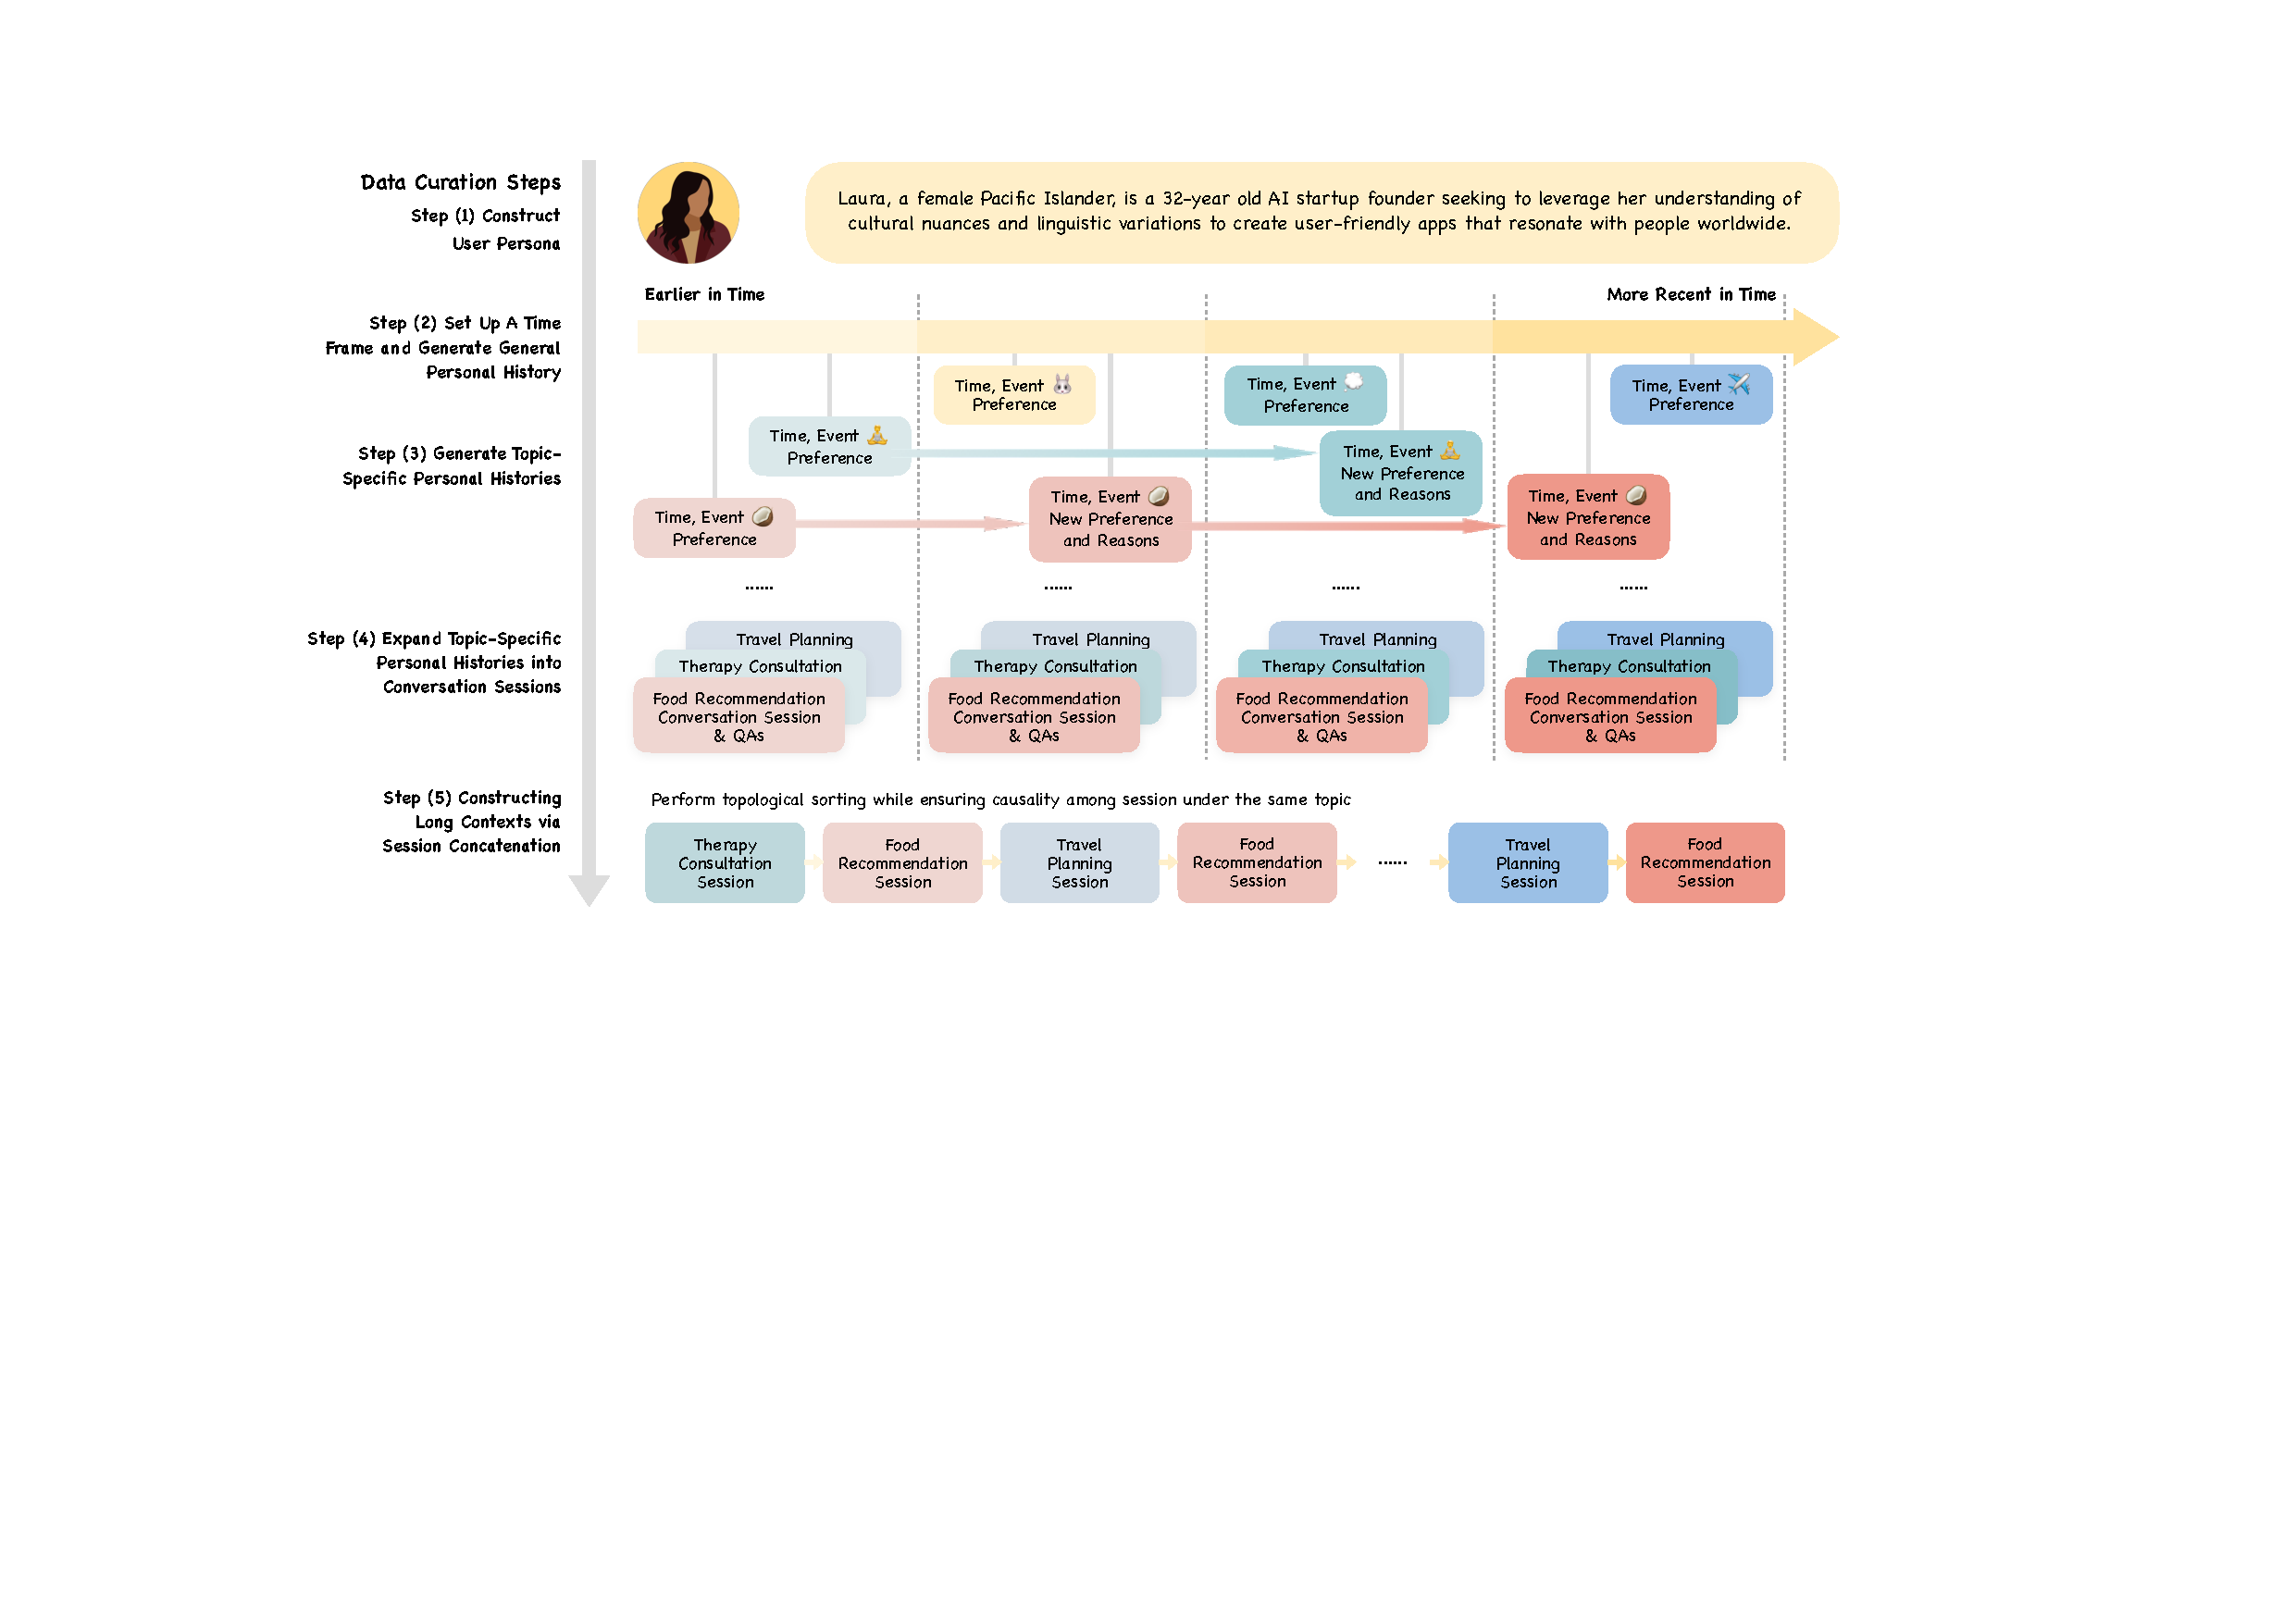
\includegraphics[width=1\linewidth]{figures/generate_data.pdf}
  \caption{\textbf{An overview of the persona-oriented multi-session data curation process}. We construct user personas, build time-stamped general and topic-specific personal histories, expand them into conversation sessions, and topologically concatenate sessions to create long conversation contexts—resulting in a scalable generation framework.}
  \vspace{-2mm}
  \label{fig:generate_data}
\end{figure}

\paragraph{Assemble interaction history via session concatenation.}
Generating large-scale, persona-oriented long-context conversations can be both \textit{cost-efficient} and \textit{scalable}. For each persona, we topologically sort conversation sessions based on their ending timestamps, and we only need to make sure sessions within the same topic maintain causality. \textit{Different numbers of sessions can be concatenated in multiple valid orders.} This flexible design allows for multiple valid interleavings of sessions across different topics, meaning \textit{we only need to generate sessions themselves—not every entire long-context conversation from scratch.} To further extend context length and simulate more natural interactions, we insert a limited number of short interactions between sessions where the user asks random knowledge questions or programming helps without indicating any user preferences.

% \subsection{Resolving the Chicken-and-Egg Dilemma}
% While we leverage GPT-4o to generate conversation data, we also evaluate language models on this generated data. This creates a potential chicken-and-egg dilemma. However, we assume that generating individual conversation sessions—especially with access to structured personal histories—is trivial. In contrast, evaluating model performance over the full, concatenated long-context conversations remains challenging.


% We aim to generate long-context conversation data extending up to one million tokens, significantly surpassing a single conversation session. To achieve this, we need a cost-effective approach for producing numerous long-context samples. Given that we have independently collected one to four conversation sessions per topic — aside from shared persona and general personal history — we can create diverse long-context samples by selecting different subsets of these sessions from multiple topics, arrange them topologically based on their ending timestamps, and concatenate them in different configurations. 

% This approach offers flexibility in constructing long-context conversations. We can concatenate any number of available sessions, and there are multiple valid ways to perform topological sorting on these sessions. Instead of generating each long-context sample from scratch, we can efficiently create multiple versions using only the existing sessions we have already generated, without making additional API calls to any large language models.

% TODO: Add explanation on the chicken-and-egg problems here


% \subsection{Curating of Question-Answering Pairs}
% We implement a multiple-choice question answering framework to evaluate the discriminative setting as mentioned in Section \ref{sec:overview}. This methodology assesses two critical aspects of model performance: comprehension of user personas and tracking of conversational evolution. During the conversation, we simulate the questions users might ask language model agents. Each evaluation item presents both correct answers and strategically designed incorrect options. These incorrect options fall into two categories: factually inaccurate statements and information not present in the conversation history.

% For user-specific recommendation problems, we construct misleading options by modifying correct responses to align with stereotypical characteristics based on general user identities while contradicting specific preferences revealed during conversations. This approach evaluates a crucial capability: the model's ability to differentiate between contextual, user-specific memory and its pre-existing parametric knowledge. Such discrimination is fundamental for effective personalized memorization.

%\subsection{Curation of Generating Personalized Conversation}
%TODO: discuss the metric and implementation for generative settings -- or should we talk about it in experiment section?

% \subsection{Curation of Persona and Event-Grounded Question and Answers}

% TODO

\paragraph{Human validation on dataset quality.}
To evaluate the quality of our generated data, we conduct a human study on 90 random query–response pairs from \datasetname, each grounded in user persona, personal histories, and associated utterances in conversation. Three annotators assess each Q\&A pair across four dimensions: appropriateness, relevance, correctness, and best response. Judgments were very high for all dimensions -- 97.8\%, 95.6\%, 97.8\%, and 90.0\% respectively. Further details are provided in Appendix~\ref{sec:human_eval}.
% To check the quality of our generated data, we perform a human evaluation on a subset of data from \datasetname. As the dataset curation process is complex, we task humans with annotating the final stage -- the questions and answers, paired with the session and metadata they are grounded in. We ask three annotators to binarily evaluate 90 entries on 4 dimensions: appropriateness, relevance, correctness, and best response. We find that the annotators rate all dimensions highly (TODO), and that agreement between them is also high (TODO). Further details are provided in Appendix~\ref{sec:human_eval}.
\section{Experiment}
% We evaluate state-of-the-art language models based on efficiency and context window limits.


\subsection{Evaluation Settings}
Given an \textit{in-situ} user query and the user's interaction history up to a point in time, we evaluate models' ability to select the most appropriate response according to the current state of the user amonst four different choices. Only one of the choices fits the user's current status, and the other choices contain either irrelevant or outdated facts or preferences from the user.   
During evaluation, apart from the conversation history, the models have access to the basic demographic information of the user, including name, age, gender identity, racial identity, and occupation. The models do not have direct access to the user's other dynamic characteristics and personal history otherwise.

For selecting the most appropriate response, we evaluate models under both discriminative and generative settings. In the \textit{discriminative setting}, the models are presented with all four response choices denoted with (a), (b), (c) and (d) with random ordering among the choices. The model is asked to output the correct choice along with a brief explanation. 
In the \textit{generative setting}, the models still see one question at a time. We compute the log-sum of token probability of generating each option individually with length normalization, and select the option with the highest probability as the model response. We use the \textit{discriminative setting} for main evaluation (\S~\ref{ssec:discriminative},\S~\ref{ssec:long-context}, \S~\ref{ssec:rag}) and adopt the \textit{generative} setting in \S~\ref{ssec:geneartive}, as it requires access to logits over entire vocabulary during decoding, which is not available from most proprietary models. No LLM judges are involved in the evaluation process. 
% This is done by autoregressively appending the tokens of each candidate answer to the model’s output and recording the logit probabilities, and the final prediction is the one with the highest joint probability after length normalization. 
% We avoid LLM-as-a-judge in favor of more robust evaluation.


\subsection{Evaluating Language Models in Long-Context Settings}
\label{ssec:discriminative}
We first evaluate language models in the long-context setting, where the full user-LLM interaction history is provided as input to the models. Due to the length of the history, all models here were evaluated zero-shot, without demonstration examples of other histories and user queries.  
% long present comprehensive results on state-of-the-art language models used out-of-the-box with direct prompting, simulating practical, everyday user scenarios.
Our evaluation covers GPT-4.1, o4-mini, o3-mini, GPT-4.5, o1, GPT-4o, GPT-4o-mini, Gemini-2.0-Flash, Gemini-2.0-Flash-Lite, Gemini-1.5-Flash, DeepSeek-R1-671B, Llama-4-Maverick, Llama-3.1-405B, Claude-3.7-Sonnet, and Claude-3.5-Haiku~\citep{openai2025gpt45, openai2024o4mini, openai2025o3mini, openai2024o1, hurst2024gpt, team2024gemini, guo2025deepseek, grattafiori2024llama, anthropic2024claude3} on 128$k$-token context windows. We also evaluate models that support longer contexts—Llama-4-Maverick, Gemini-2.0-Flash, Gemini-2.0-Flash-Lite, and Gemini-1.5-Flash—on 1$M$-token context windows. 
We report the following findings:


\begin{figure}[t]
  \centering
  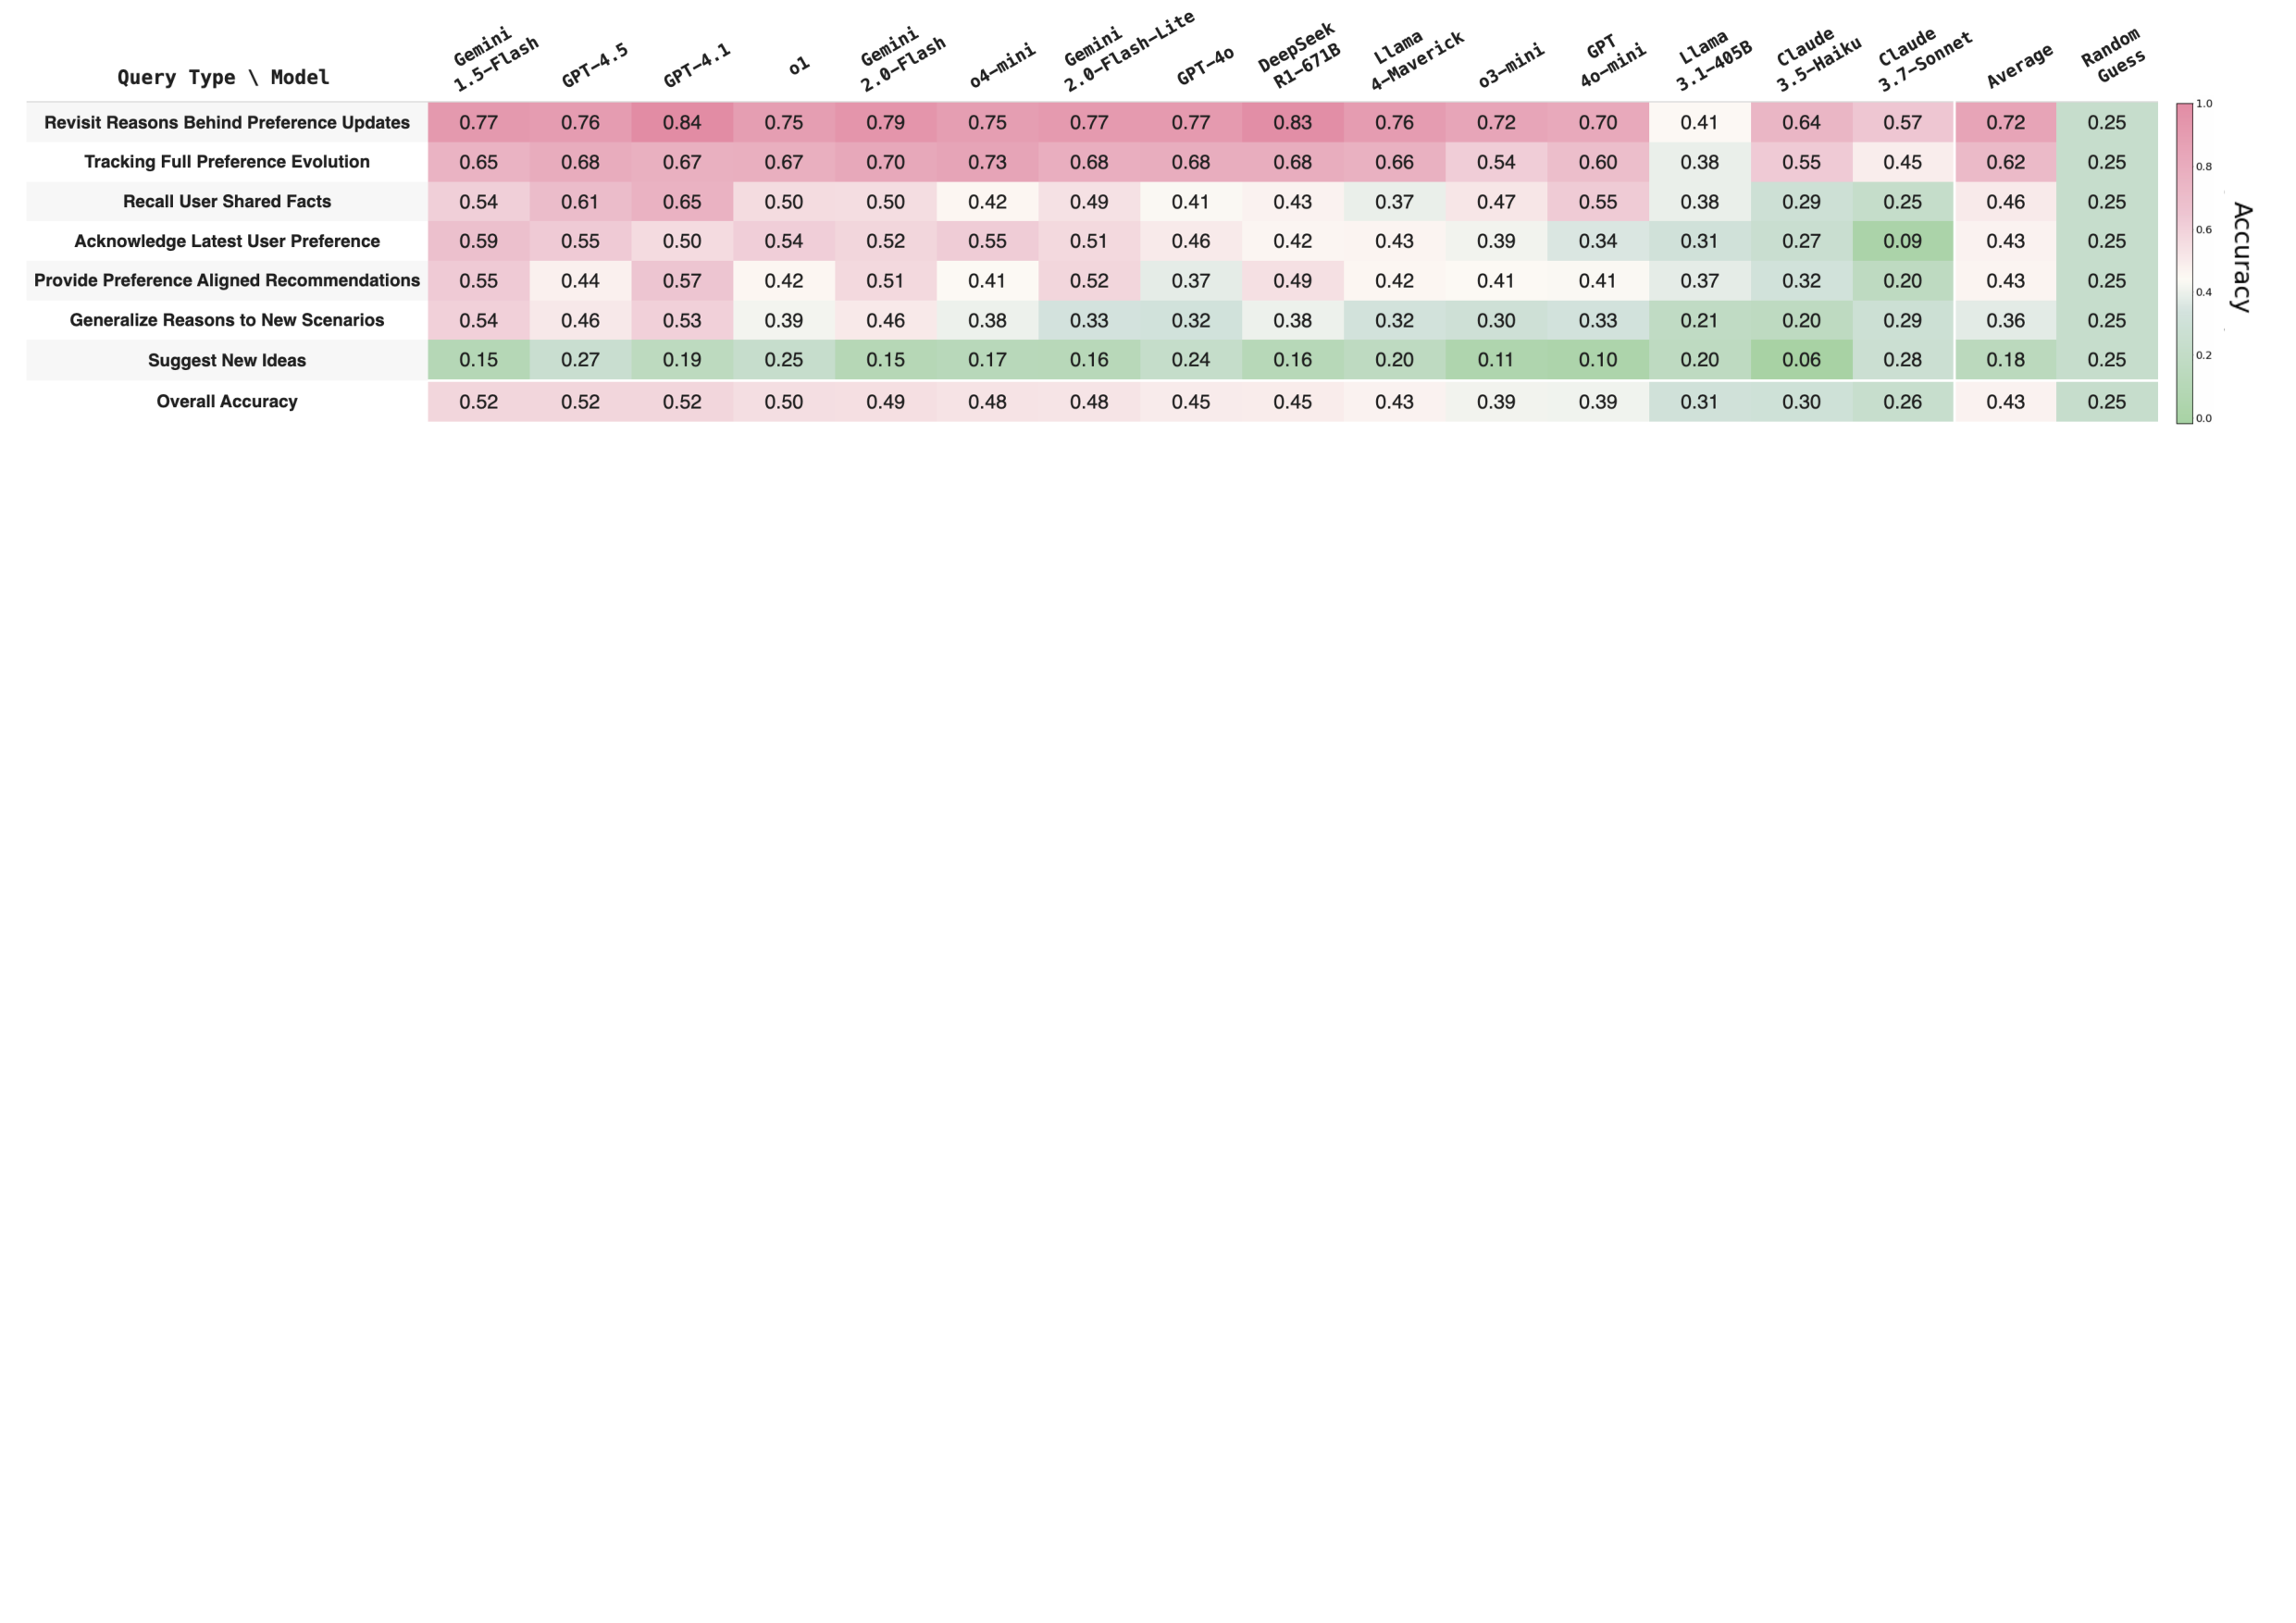
\includegraphics[width=1\linewidth]{figures/results_qa_types.pdf}
  \caption{Evaluation results across different models on 7 \emph{in-situ} query types. 
  % designed to test their ability to reason about user preferences, including acknowledging user facts, tracking preference changes, and generating aligned recommendations. 
  We observe models perform reasonably well at recalling user facts and preferences. However, models struggle at providing novel suggestions, or applying users' preferences in new scenarios.}
  % \vspace{-5mm}
  \label{fig:128k_qa_types}
\end{figure}

\begin{figure}[t]
  \centering
  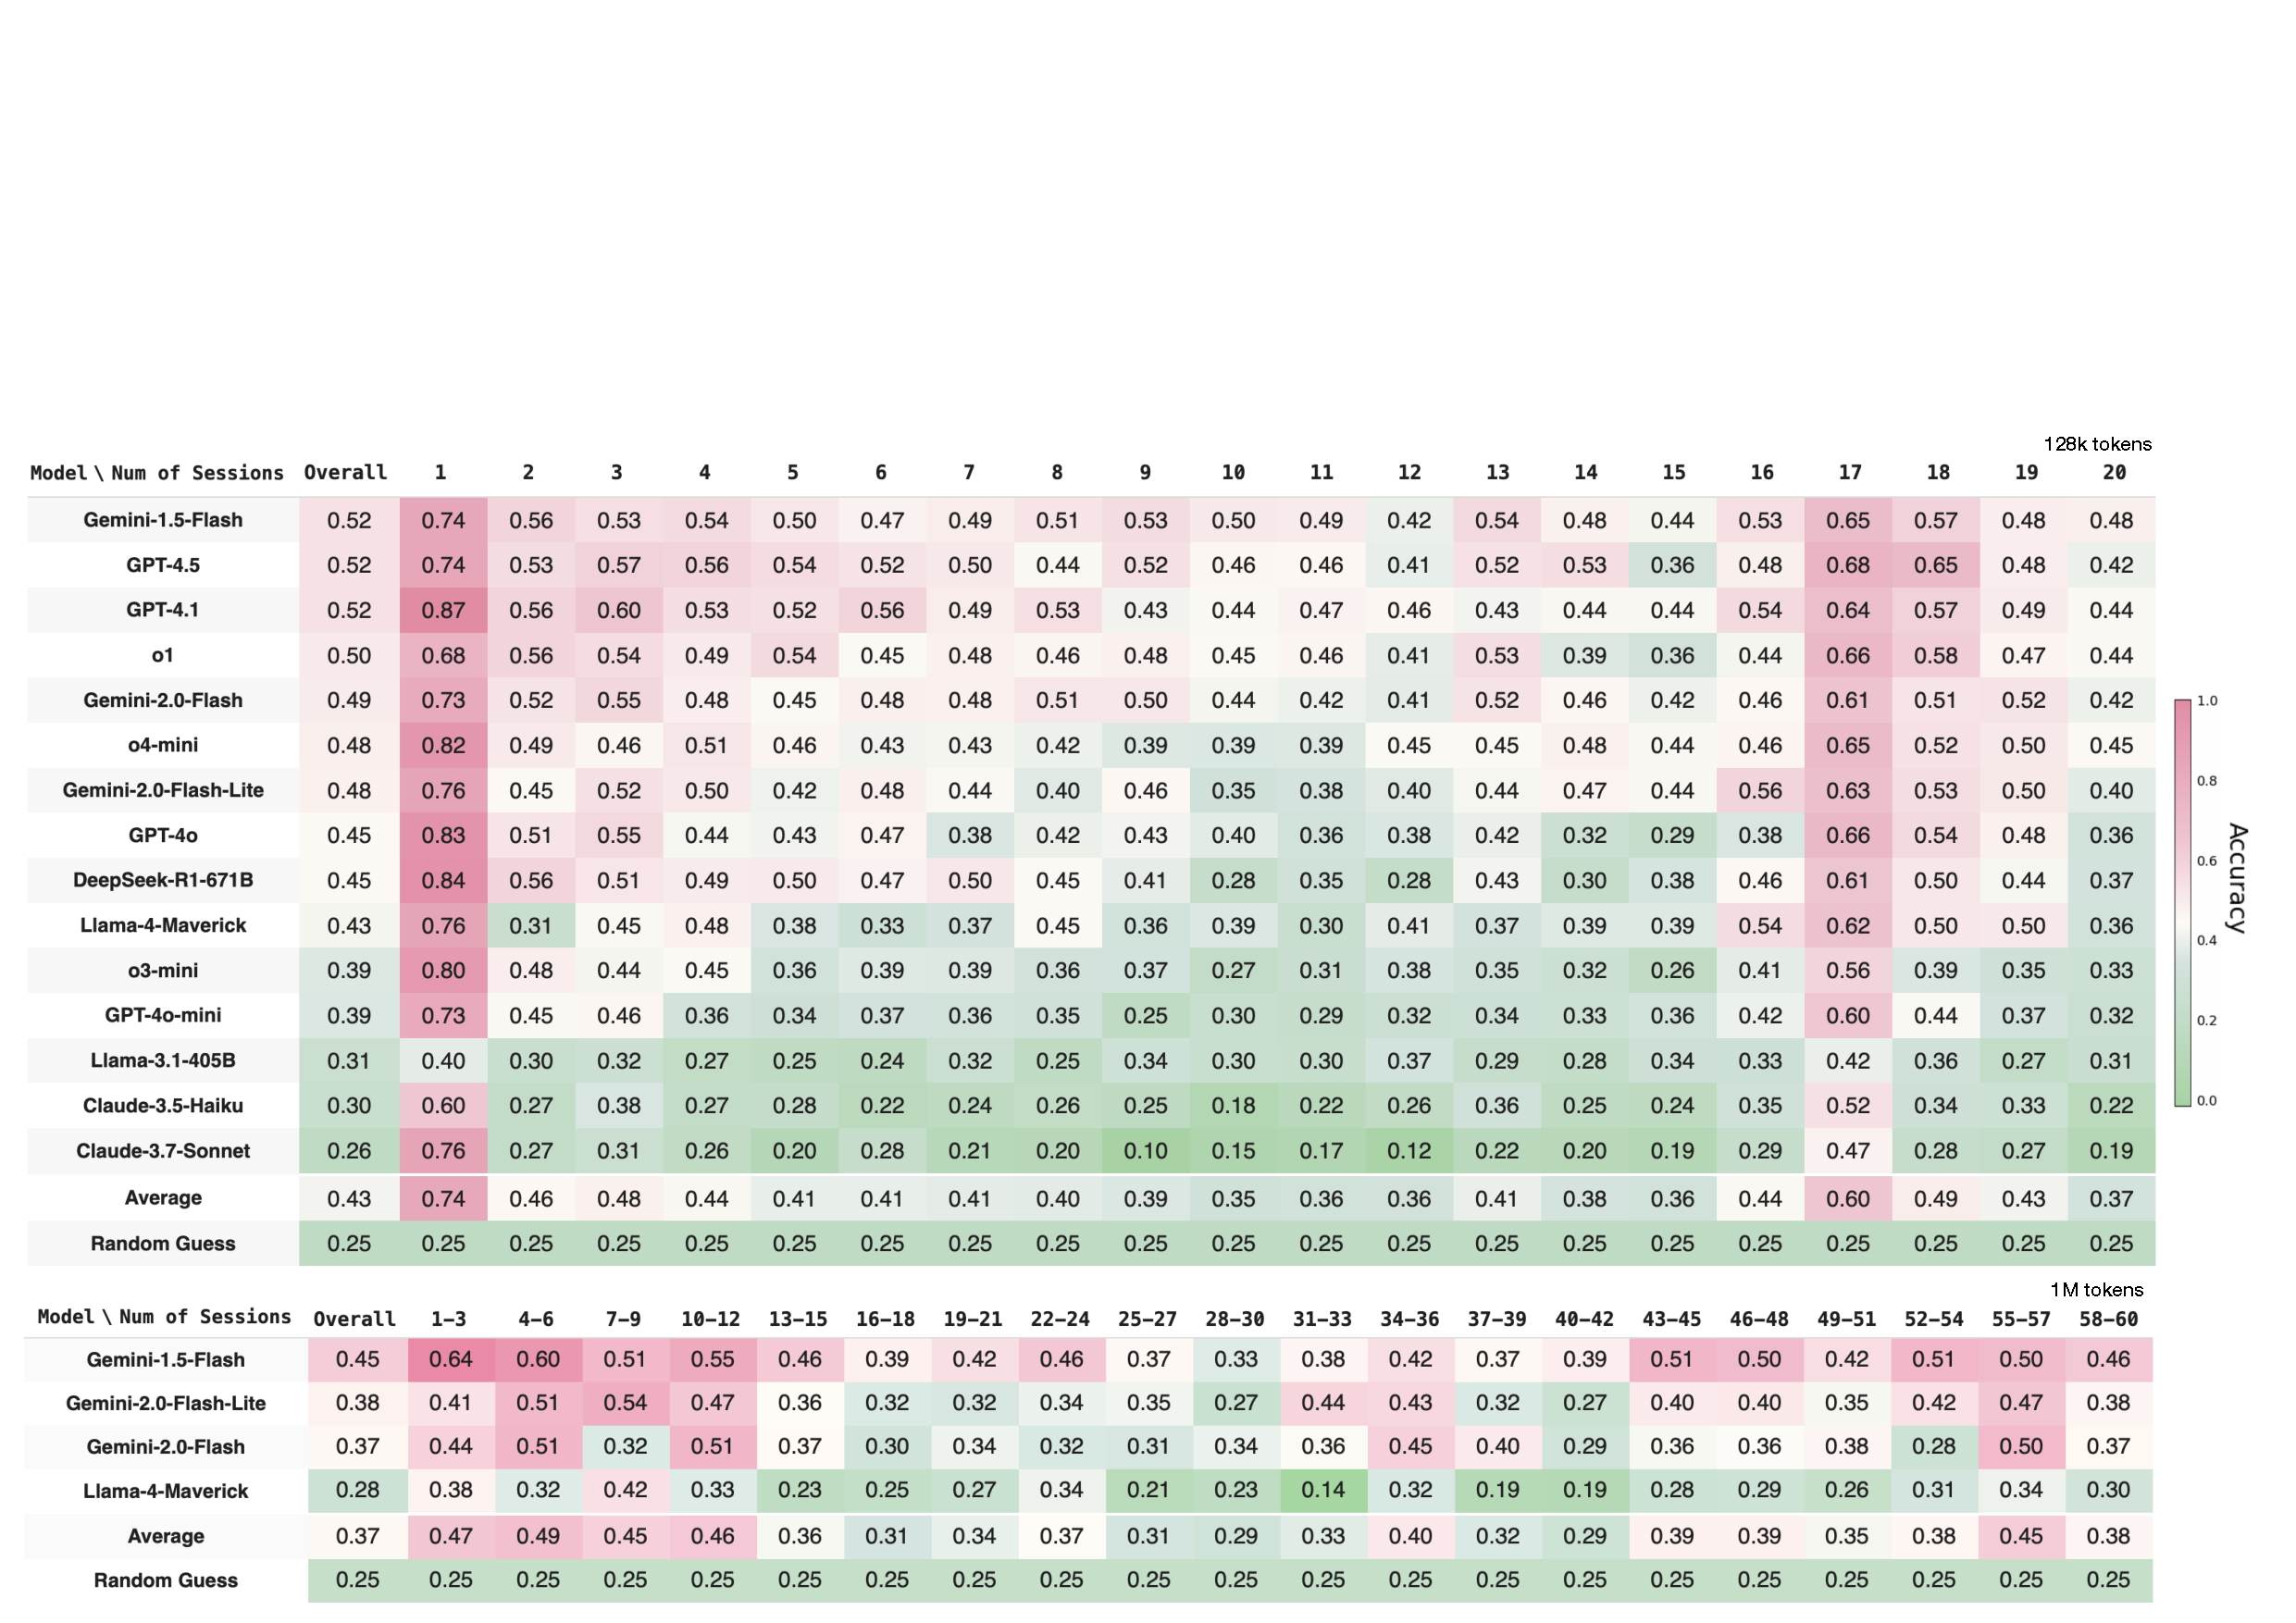
\includegraphics[width=1\linewidth]{figures/results_long_context.pdf}
  \caption{Model performances by number of sessions elapsed since most recent preferences were mentioned in long context. Top: up to 20 sessions/128k tokens; Bottom: up to 60 sessions/1M tokens. Long-context retrieval is important for personalization in practice.}
  % \vspace{-5mm}
  \label{fig:long_context}
\end{figure}




\paragraph{GPT-4.5, GPT-4.1, and Gemini-1.5 achieve the highest overall performance.}
Among leading foundation models, GPT-4.5 and Gemini-1.5 outperform others in overall accuracy. However, their performance still hovers around 52\% in a multiple-choice setting, highlighting substantial room for improvement. \textbf{Notably, reasoning models such as o1, o3-mini, o4-mini, and DeepSeek-R1-607B do not demonstrate competitive advantages over non-reasoning models in the personalization tasks we evaluate.}
% capabilities alone are insufficient for effective personalization, as demonstrated by advanced reasoning models such as o3-mini, o1, and DeepSeek-R1-607B. %We also observe a slight performance decline in the Gemini-2 series compared to Gemini-1.5. 

\paragraph{LLMs demonstrate reasonably good performance in recalling simple user facts.}
    For tasks involving the retrieval of static user information, such as previously mentioned items, activities, or reasons behind preference changes where the reasons themselves won't change, most LLMs have a reasonable chance of succeeding.
    
\paragraph{Incorporating the latest user preference into responses is more challenging than recalling the change in user profile.} We observe that models struggle to incorporate the latest preference or state of the user in responses. Surprisingly, models generally get higher performance when asked to recall how the user preferences evolve over time. 
We observe that asking the model to iterate through all preference updates may encourage it to think through the preference evolutions, often making the task easier.
    
\paragraph{Models fall short on generating new ideas or providing suggestions in new scenarios.}
    As shown in Figure~\ref{fig:128k_qa_types}, tasks such as \textit{"Suggest New Ideas}", \textit{"Provide Preference-Aligned Recommendations"}, and \textit{"Generalize Reasons to New Scenarios"} yield the lowest performance across all models, highlighting the challenge of generating personalized responses in novel contexts—particularly when identifying new facts.


\subsection{Effect from the Position of User Information in Interaction History}
\label{ssec:long-context}
To understand how the model performance is affected by the position in which the relevant user facts or preferences appear in the conversation history, we report the model performance by the session in which the relevant user information appears in the history. The results are shown in Figure~\ref{fig:long_context}. Generally, we observe that the model performs better when the relevant information appears in the earler or later sessions of the conversation history. The findings here generally echo previous findings on long-context inputs to models, where context information tends to get ``lost in the middle'' \citep{liu2024lost, wu2024longmemeval}.     

    % As shown in Figure~\ref{fig:long_context}, personalization under long context windows remains difficult, particularly for user information that appears far from the end of the context, indicating that long-context retrieval is important for achieving strong personalization in practice.
    



% \begin{table*}[ht]
% \centering
% \small
% \resizebox{\textwidth}{!}{%
% \begin{tabular}{lcccccccc}
% \toprule
% \textbf{Model} & 
% \makecell[c]{\textbf{Overall}} & 
% \makecell[c]{\textbf{Revisiting} \\ \textbf{Previous} \\ \textbf{Reasons}} & 
% \makecell[c]{\textbf{Tracking} \\ \textbf{Full} \\ \textbf{Evolution}} & 
% \makecell[c]{\textbf{Incorporating} \\ \textbf{Latest} \\ \textbf{Preference}} & 
% \makecell[c]{\textbf{Incorporating} \\ \textbf{User Shared} \\ \textbf{Facts}} & 
% \makecell[c]{\textbf{Preference} \\ \textbf{Aligned} \\ \textbf{Recommendations}} & 
% \makecell[c]{\textbf{Generalizing} \\ \textbf{Reason to} \\ \textbf{New Scenarios}} & 
% \makecell[c]{\textbf{Identifying} \\ \textbf{Facts Not} \\ \textbf{Shared Before}} \\
% \midrule
% Gemini-1.5-Flash        & \textcolor{red}{\textbf{0.52}} & 0.77 & 0.65 & 0.59 & 0.54 & 0.55 & \textcolor{red}{\textbf{0.54}} & 0.15 \\
% GPT-4.5                 & \textcolor{red}{\textbf{0.52}} & 0.76 & 0.68 & \textcolor{red}{\textbf{0.76}} & \textcolor{red}{\textbf{0.61}} & 0.44 & 0.46 & \textcolor{red}{\textbf{0.27}} \\
% o1                      & 0.50 & 0.75 & 0.67 & 0.54 & 0.50 & 0.42 & 0.39 & 0.25 \\
% Gemini-2.0-Flash        & 0.49 & 0.79 & \textcolor{red}{\textbf{0.70}} & 0.52 & 0.50 & 0.51 & 0.46 & 0.15 \\
% Gemini-2.0-Flash-Lite   & 0.48 & 0.72 & 0.68 & 0.50 & 0.51 & \textcolor{red}{\textbf{0.52}} & 0.33 & 0.16 \\
% GPT-4o                  & 0.45 & 0.77 & 0.67 & 0.46 & 0.41 & 0.37 & 0.32 & 0.24 \\
% DeepSeek-R1-67B         & 0.45 & \textcolor{red}{\textbf{0.83}} & 0.68 & 0.42 & 0.43 & 0.49 & 0.38 & 0.16 \\
% o3-mini                 & 0.39 & 0.76 & 0.60 & 0.40 & 0.40 & 0.41 & 0.31 & 0.14 \\
% GPT-4o-mini             & 0.39 & 0.70 & 0.60 & 0.34 & \textcolor{red}{\textbf{0.55}} & 0.41 & 0.33 & 0.10 \\
% LLaMA-3-405B            & 0.31 & 0.41 & 0.38 & 0.31 & 0.38 & 0.37 & 0.21 & 0.20 \\
% Claude-3.5-Haiku        & 0.30 & 0.65 & 0.34 & 0.24 & 0.29 & 0.20 & 0.22 & 0.06 \\
% Claude-3.7-Sonnet       & 0.26 & 0.57 & 0.45 & 0.09 & 0.25 & 0.20 & 0.29 & 0.09 \\
% \midrule
% \textbf{Average Accuracy} & \textbf{0.420} & \textbf{0.694} & \textbf{0.548} & \textbf{0.456} & \textbf{0.434} & \textbf{0.404} & \textbf{0.359} & \textbf{0.163} \\
% Random Guess            & 0.25 & 0.25 & 0.25 & 0.25 & 0.25 & 0.25 & 0.25 & 0.25 \\
% \bottomrule
% \end{tabular}
% }
% \caption{Prompt: Model performance across multiple reasoning skills. "Overall" is placed first; other columns are sorted by average accuracy (excluding Random Guess) in descending order. Maximum per column is bold and red. Average accuracy row is shown just above Random Guess.[\textcolor{red}{TODO}: transform other result tables using this prompt]}
% \label{tab:multi_skill_eval_sorted_desc}
% \end{table*}



% \begin{figure}[t]
%   \centering
%   \includegraphics[width=1\linewidth]{figures/results_1m_sessions.png}
%   \caption{TODO}
%   % \vspace{-5mm}
%   \label{fig:1m_sessions}
% \end{figure}


\subsection{Evaluation with External Memory Modules}
\label{ssec:rag}

% \begin{figure}[t]
%   \centering
%   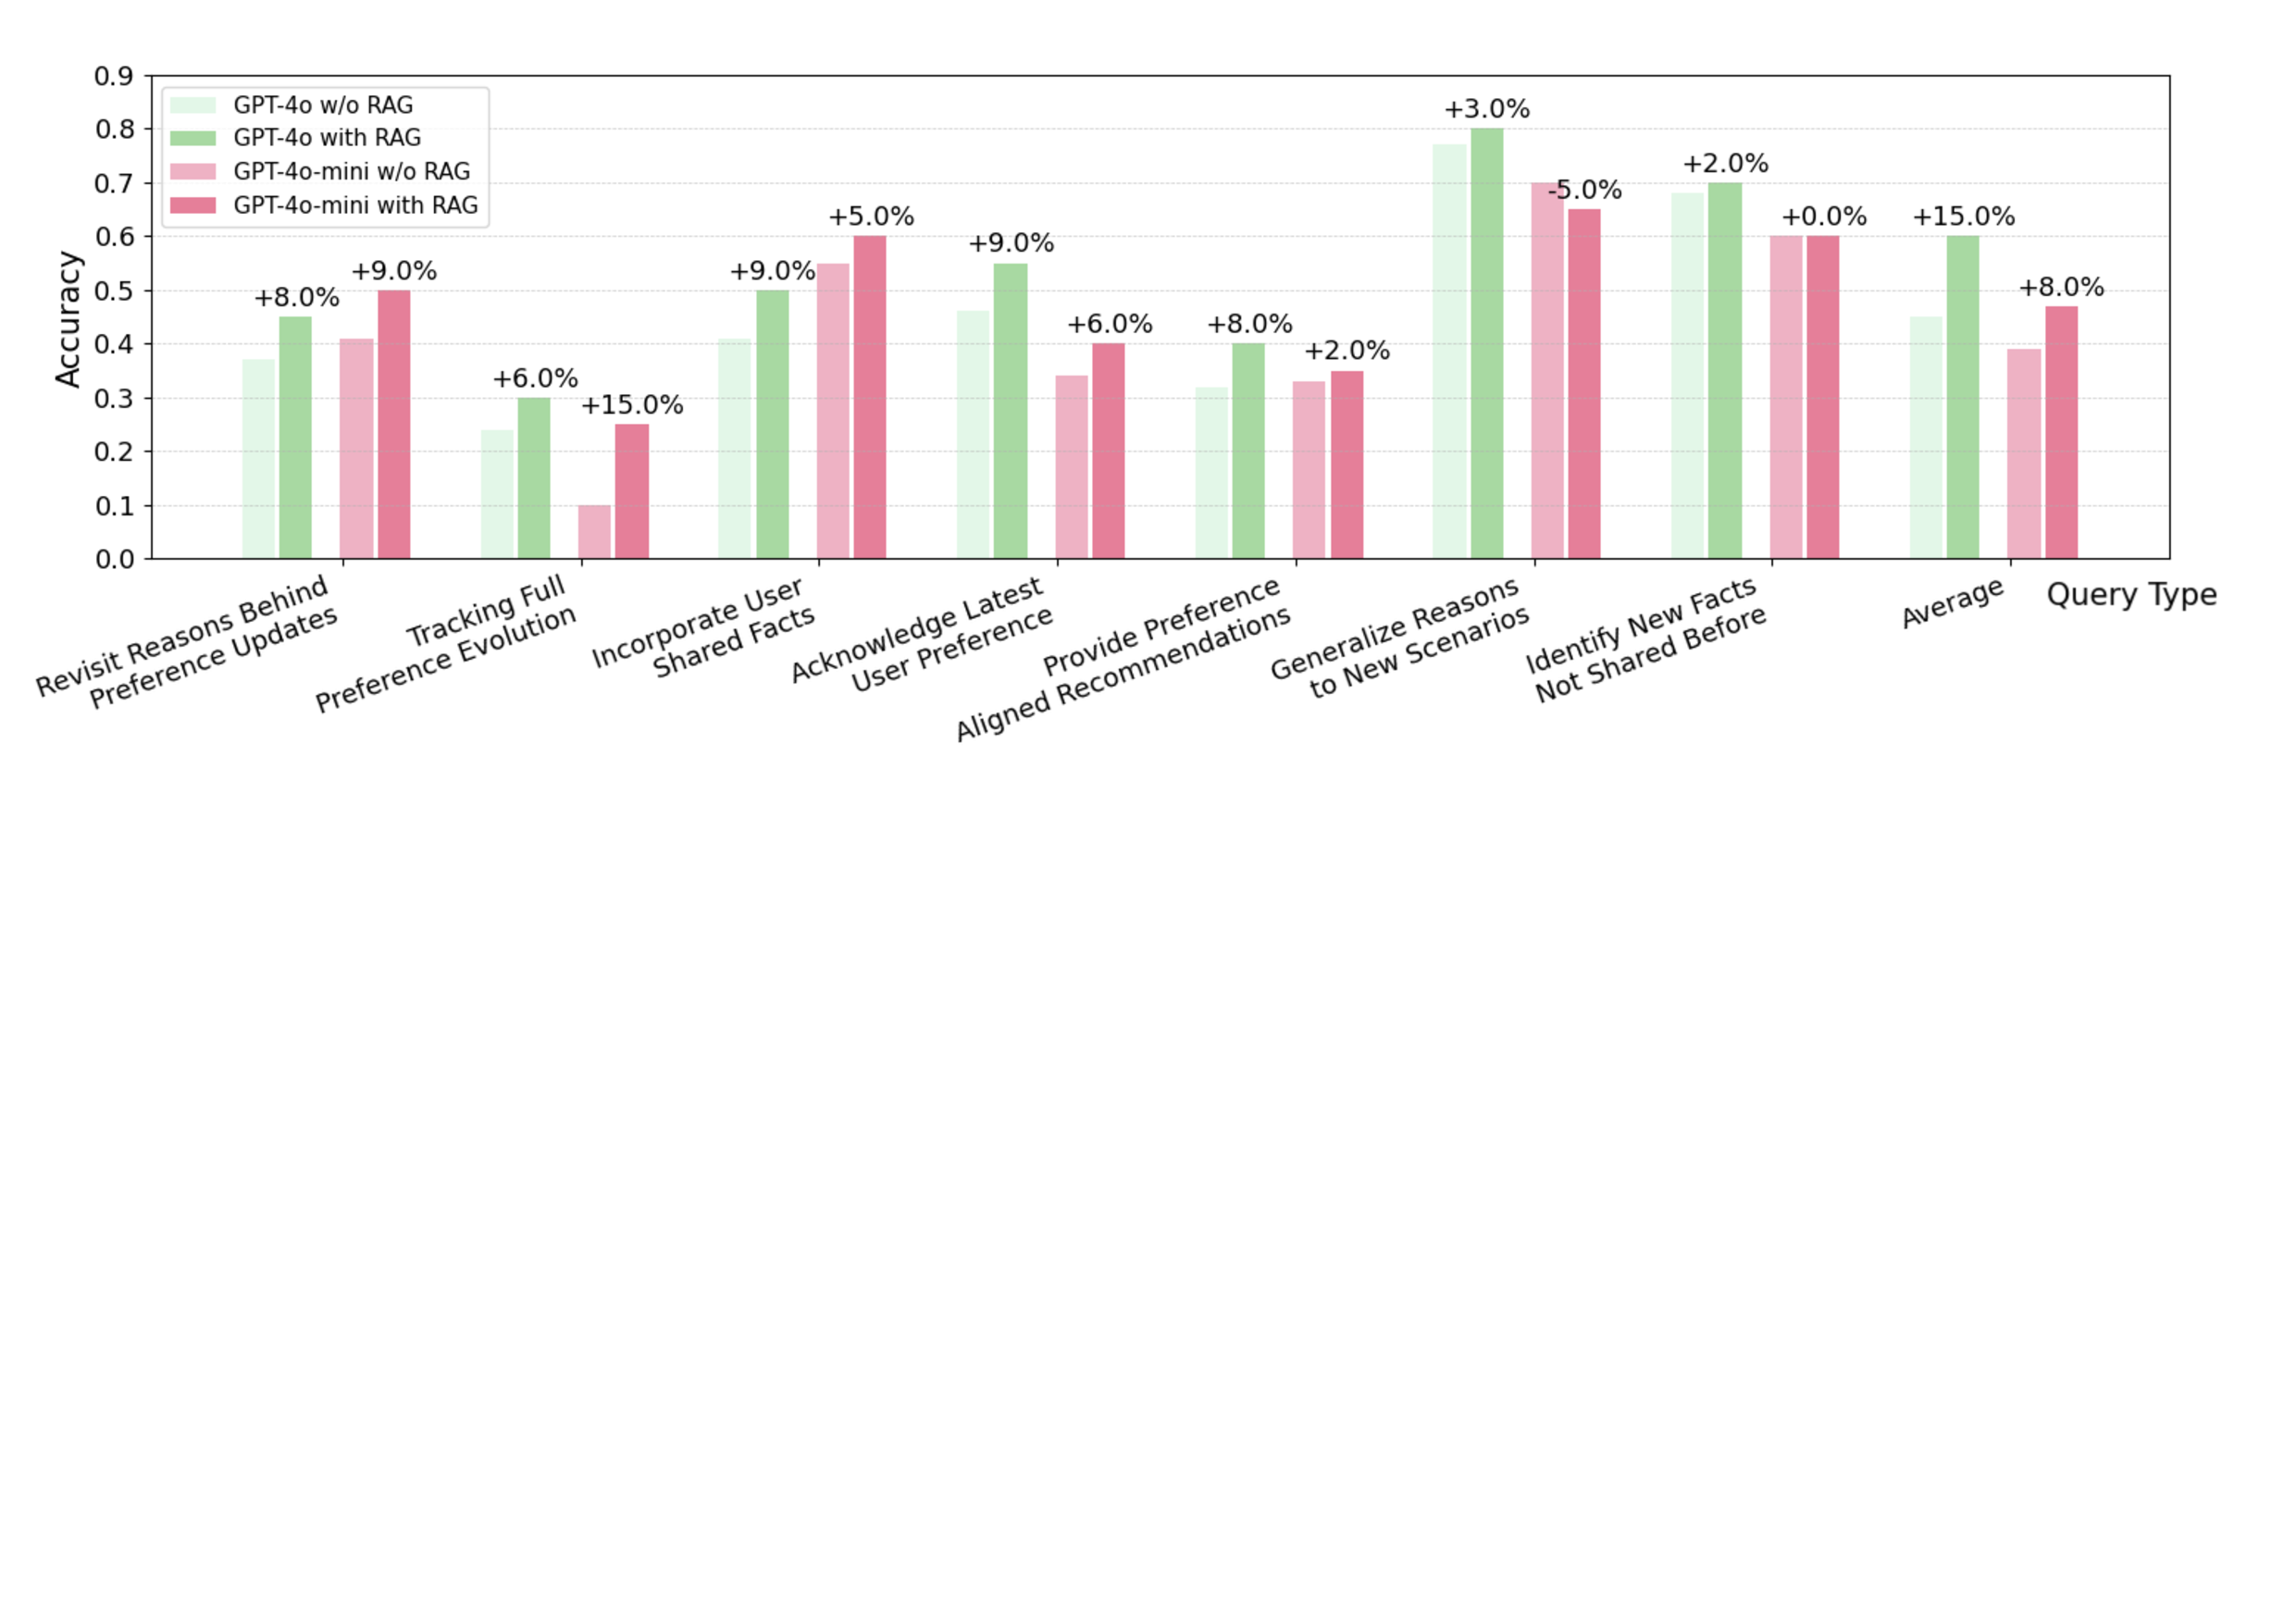
\includegraphics[width=1\linewidth]{figures/rag_128k.pdf}
%   \caption{Performance on the different question types for GPT-4o and GPT-4o-mini on the 128k context setting, and comparing with RAG to without RAG. We observe that overall RAG improves accuracy across types and models. Most notable boosts are for `Tracking Full Preference Evolution'. However, as expected, it fails to assist in the types involving new information.}
%   % \vspace{-5mm}
%   \label{fig:rag_128k}
% \end{figure}

\begin{figure}[t]
  \centering
  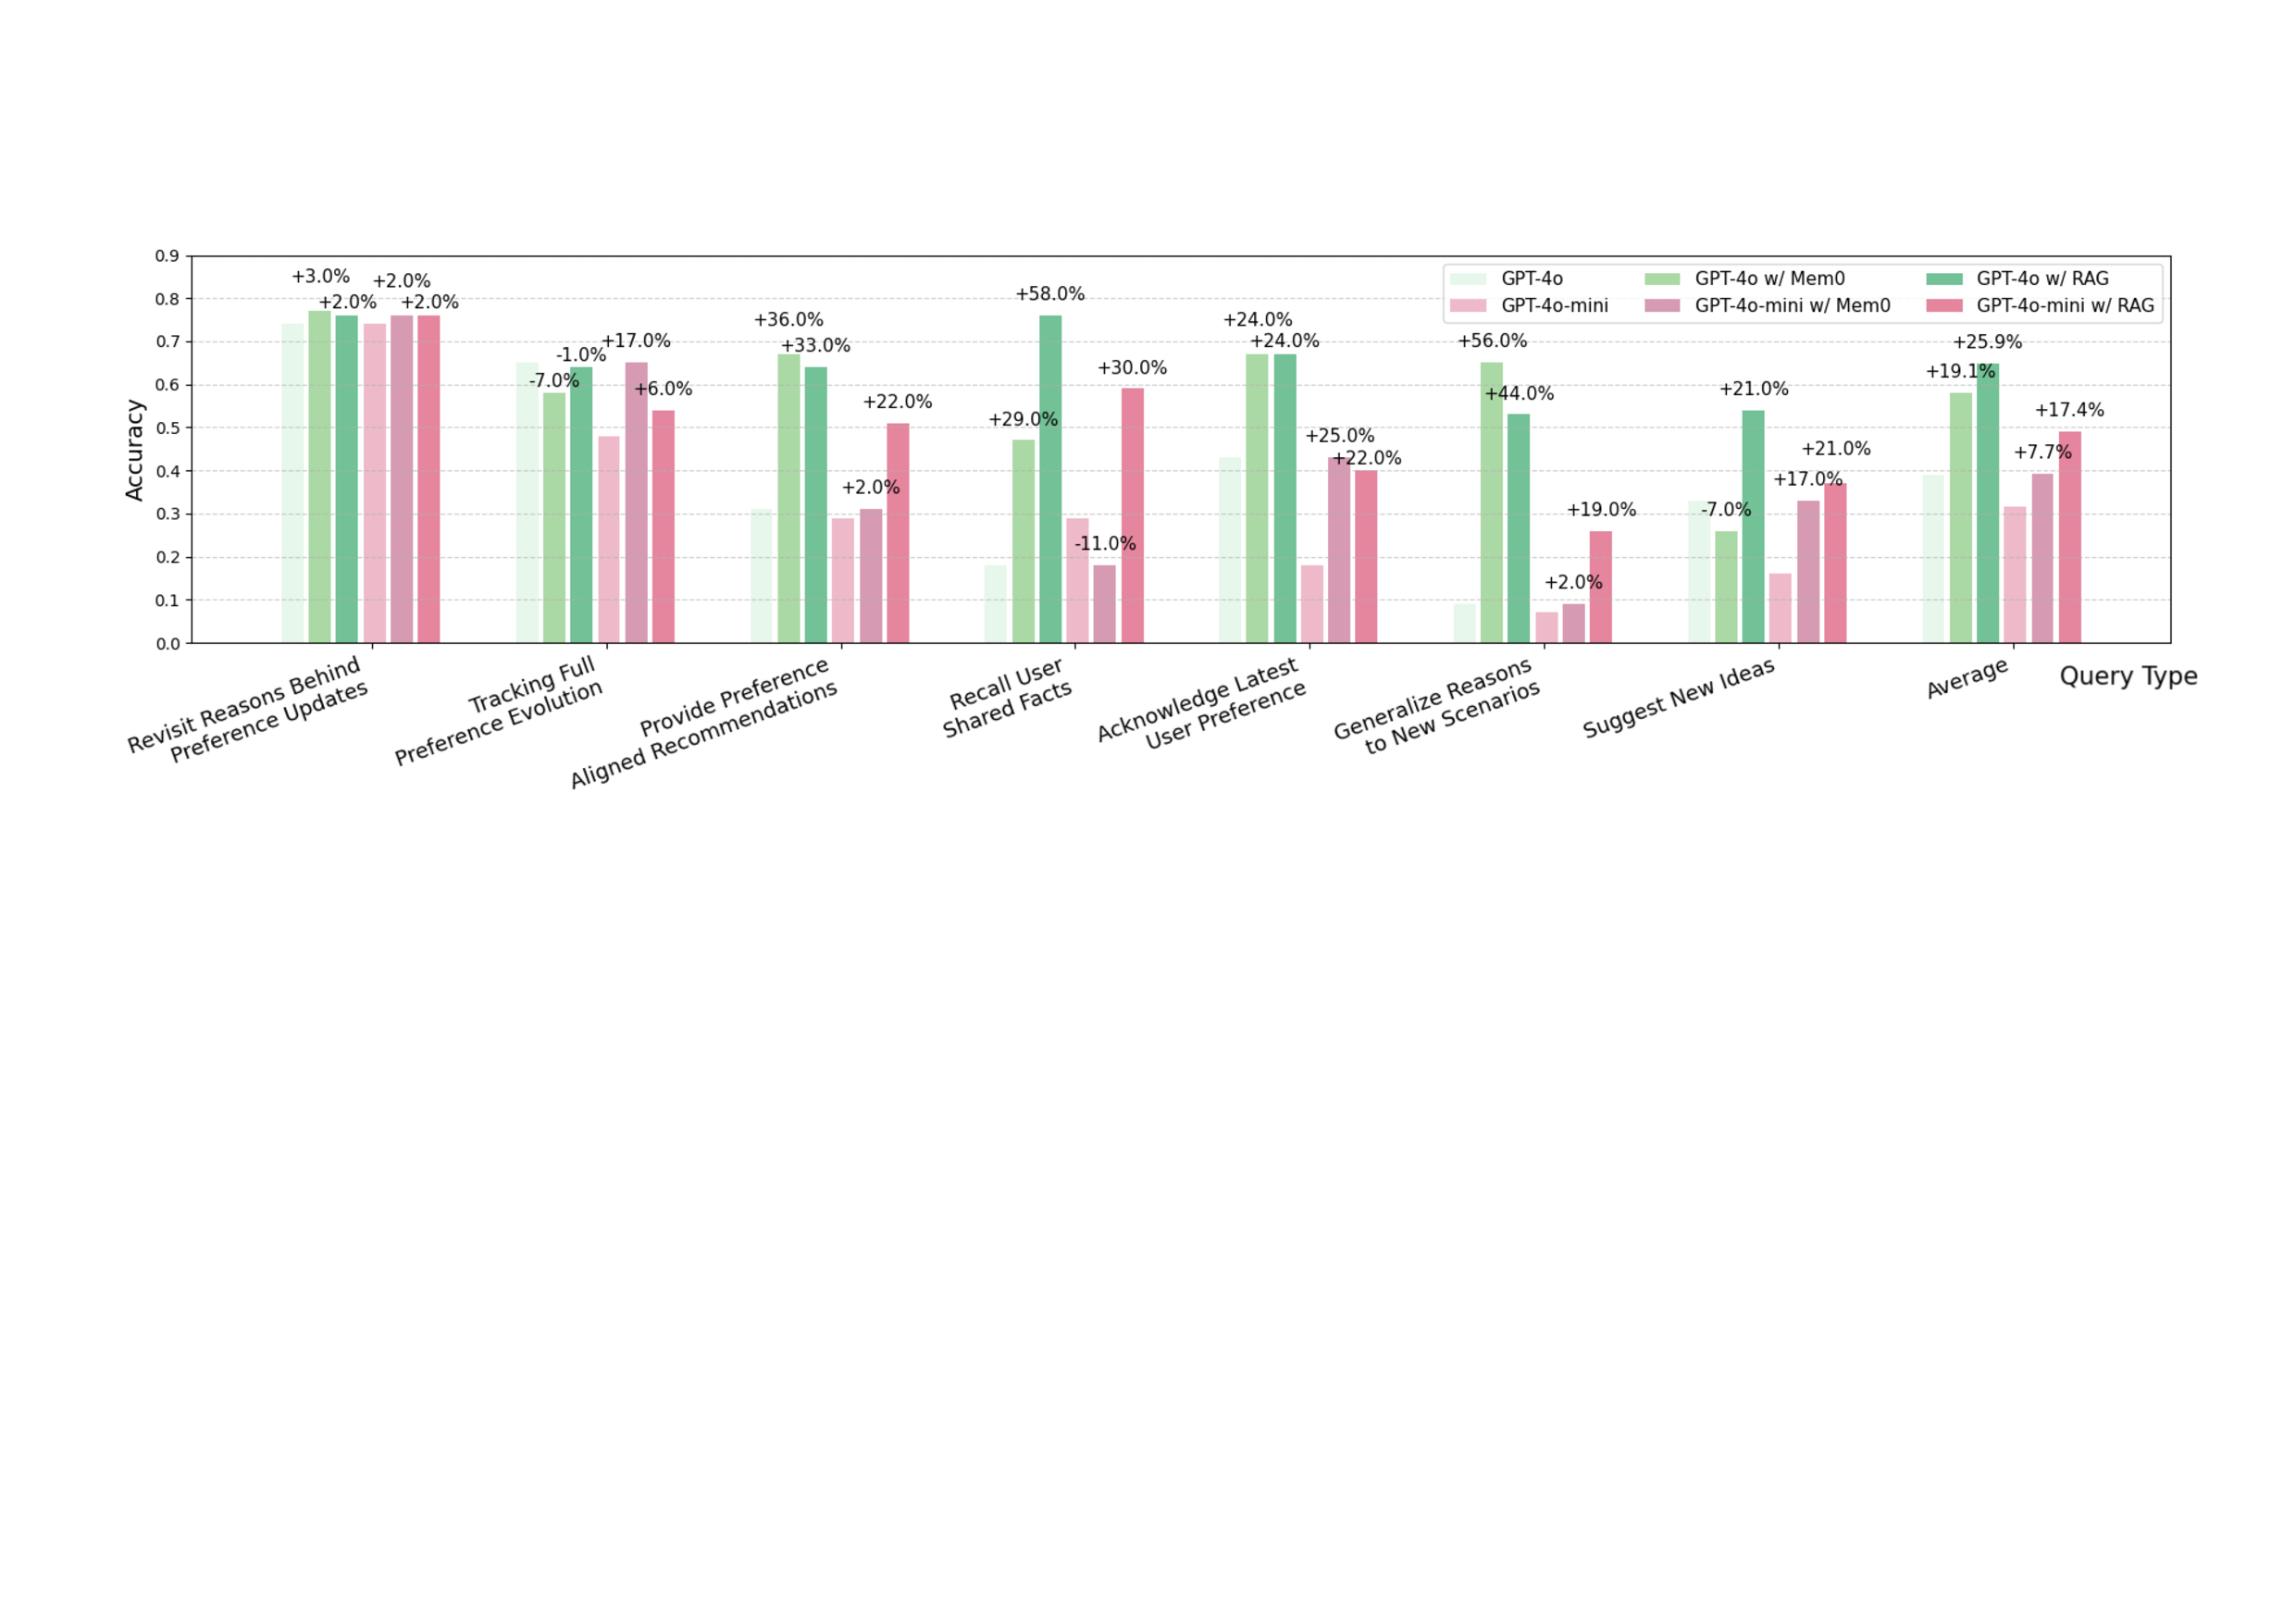
\includegraphics[width=1\linewidth]{figures/rag_mem0_32k.pdf}
  \caption{Performance on different question types for GPT-4o and GPT-4o-mini with 32k-token contexts. We compare vanilla models to the ones with Mem0 and RAG setups.}
  \vspace{-2mm}
  \label{fig:rag_mem0_32k}
\end{figure}




% , including Retrieval Augmented Generation (RAG) and external memory modules. 

% \subsubsection{RAG-based Evaluation}
% \paragraph{Models} 
% \paragraph{Approaches}
We evaluate whether using a retriever to identify relevant information in the history will help improve model's performance.
% To understand the impact of retrieval modules,
We evaluate two external memory approaches—RAG~\citep{lewis2020retrieval} and Mem0~\citep{mem0}—against vanilla LLMs. For these experiments, we consider only the GPT-4o and GPT-4o-mini models. We show their latency in Appendix~\ref{app:latency}.

For RAG, we consider a straightforward implementation that retrieves the top five most relevant messages per question using dense BGE-M3 embeddings~\citep{chen2024bge}. For Mem0 which provides an additional memory layer to LLMs, we iteratively build a memory database using LLM-generated facts over each turn. At inference, we retrieve the top 5 relevant facts per question. For efficiency, we use 32k-token contexts for evaluation.



% We first consider a straightforward implementation of Retrieval Augmented Generation (RAG). Given an input context we retrieve the 5 most relevant messages with respect to a given question. We use BGE-M3 embeddings with the dense retrieval approach~\citep{chen2024bge}. 

% For Mem0 that provides an additional memory layer to LLMs, we iteratively build a memory database using LLM-generated facts over each turn. At inference, we retrieve the top 5 relevant facts per question. 


% evaluate GPT-4o and GPT-4o-mini models, both with and without RAG modules, across context windows of 32k and 128k tokens. For our RAG implementation, we adopt a straightforward method: for each question, we retrieve the five most similar messages from the context window using dense M3 embeddings \citep{chen2024bge}. These retrieved messages are then provided to the LLM alongside the question and its answer options to produce predictions.

% We also consider Mem0, an open-source package that adds a memory layer for LLMs \citep{mem0}. It operates by using LLM prompts to dynamically update a database of user facts; we do so iteratively over each turn in the context. Similarly to RAG, we retrieve the top 5 most relevant facts with respect to a given question.

% We compare the above two external memory approaches with the default full context setting, which passes the entire context alongside quesitons and options to LLMs.

% \paragraph{Results} 
\paragraph{Retriever-based memory module can improve model performance. }
Overall, external memory modules significantly improve accuracy for both models. Notably, \textit{Recall User-Shared Facts} and \textit{Generalize to New Scenarios} benefit the most, highlighting the effectiveness of retrieval in factual tasks. In contrast, \textit{Revisit Reasons Behind Preference Updates} shows smaller gains. RAG consistently outperforms Mem0 across most question types, although Mem0 is more computational expensive, suggesting that retrieving semantically similar messages is more effective for personalized reasoning.


% We show the performance of different approaches with a 32K context setting in Table \ref{fig:rag_mem0_32k}. Overall, using an external memory module significantly increases performance in both LLMs. Notably, performance on Recall User-Shared Facts and Generalize to New Scenarios questions shows a substantial improvement compared to the full context method, demonstrating effectiveness in handling factual questions. On the other hand, Revisit Reasons Behind Preference Updates and Track Full Preference Evolution only show marginal gains or even decreased accuracy, which indicates a need for broader memory coverage. Notably, RAG outperformed Mem0 in most of the question types, suggesting that retrieving semantically close messages to questions can be effective in solving personalized problems. Furthermore, gpt-4o with RAG on a 128K context setting achieved the highest accuracy of 59.8\%, demonstrating robustness under extremely high context lengths.

% \subsubsection{Memory-Augmented Evaluation}
% \paragraph{Models} 
% We explore Mem0~\citep{mem0}—an additional memory layer for language models—using GPT-4o and GPT-4o-mini within a 32$k$ token context window.
% \paragraph{Results}

\subsection{Evaluation of Language Models in Generative Settings}
\label{ssec:geneartive}
In real-world use cases, the chatbots do not have access to the potential options of responses during inference. For such reason, we additionally evaluate models on the more realistic \emph{generative} settings, where the model sees only one option at a time, and the best response is selected by the joint sequence probability of options from model predictions.    

% While multiple-choice question answering (MCQ) tasks effectively assess a model's ability to select appropriate responses from predefined options, they do not fully reflect realistic user interactions with language models. In practical scenarios, users rarely present multiple candidate answers but instead engage in natural conversations. To bridge this gap, we propose to evaluate whether LLMs can generate personalized responses directly in response to user queries rather than prompting the model to choose explicitly from given candidates 


\paragraph{Approaches.} 
Given the user-LLM history and in-situ user query, we compare the joint sequence probabilities by taking the log-sum of the token-level probability of each response option. 
% for each query-answer pair. 
Specifically, given a conversation history (denoted as \( \mathcal{C} \)) and the user query (\( q \)), we evaluate each candidate response $r_{i \in \{1, 2, 3, 4\}}$, consisting of tokens \( \{x_i^1, x_i^2, \dots, x_i^{T_l}\} \) of total token length $l$. Due to the \textit{autoregressive} nature of causal language models, the joint log probability for each query-answer pair is computed by summing the conditional log probabilities of each token given its preceding context, formalized as 
% $\log P(r_i \mid \mathcal{C}, q) = \sum_{t=1}^{T_i} \log P(x_i^t \mid \mathcal{C}, q, x_i^1, \dots, x_i^{t-1})$.
\vspace{-1mm}
\[
\log P(r_i \mid \mathcal{C}, q) = \sum_{t=1}^{T_i} \log P(x_i^t \mid \mathcal{C}, q, x_i^1, \dots, x_i^{t-1})/T_i
\]
\vspace{-3mm}

As the method requires logarithmic probability of output tokens over the entire vocabulary, which is often not available in proprietary models, we evaluate open-weight models—LLaMA-3.1–70B, LLaMA-3.1–8B, and DeepSeek-Distill-LLaMA–8B. Due to constraints in computation resources, we only evaluate the models on the 10-session version of the benchmark, which includes around 32$k$-tokens per session.

\paragraph{Results.} As shown in Figure \ref{fig:generative}, we observe the similar trend to our \emph{discriminative} evaluation results in terms of difficulty by different user query types. Models get reasonably good performance on recalling facts and tracking preference changes, while giving new suggestions and generalizing to new scenarios are still the most challenging types of queries for models. Interestingly, when comparing the same model, specifically LLama-3.1-8B-instruct, under discriminative and generative settings, we see the performance is better in the generative setting, potentially suggesting that the model is able to provide a personalized response without seeing all the candidate options in the input. Since we only managed to run evaluation on 32k context length with the generative setting, it remains to be investigated whether results in \textit{generative} vs. \textit{discriminative} settings stand for longer context length and for different models. We also find that model performance declines as users’ new requests become more distant from their previously revealed information. Detailed results are provided in Appendix \ref{sec:generative_session}.
\begin{figure}[t]
  \centering
  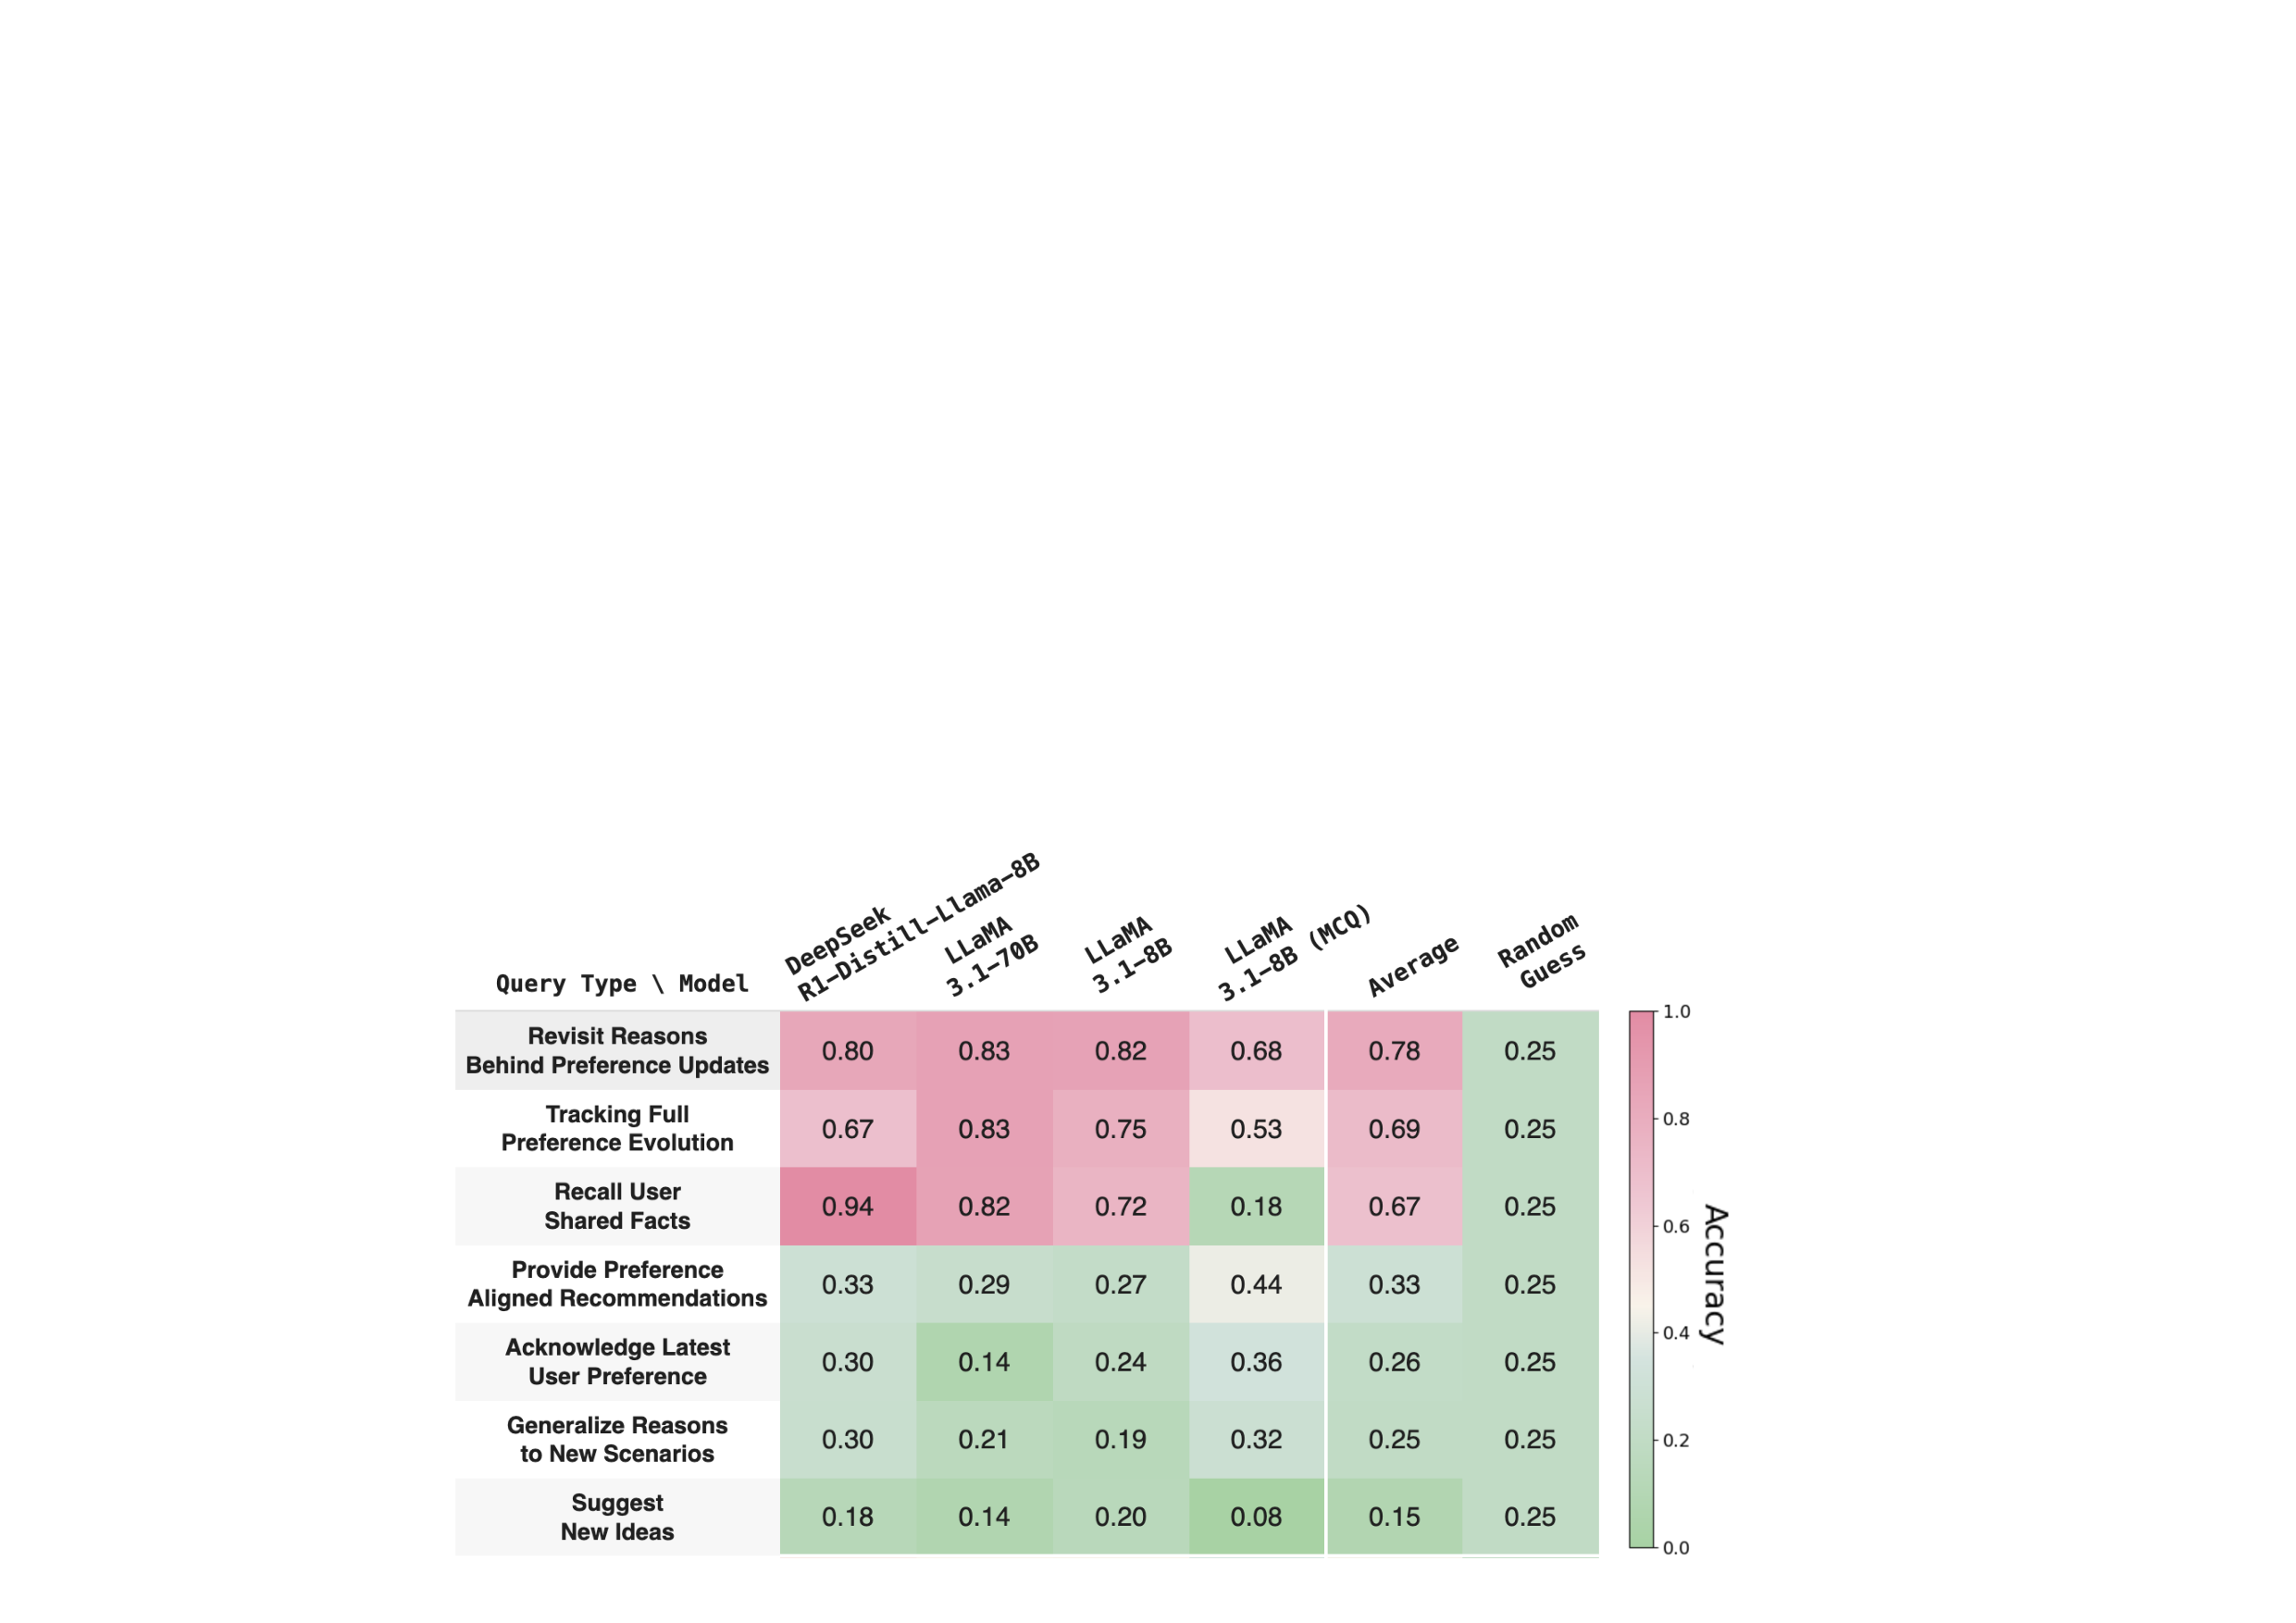
\includegraphics[width=0.53\linewidth]{figures/results_generative.pdf}
  \caption{Generative evaluation on 10-session (32k token length) version of \datasetname.}
  \vspace{-5mm}
  \label{fig:generative}
\end{figure}

% \begin{figure}[t]
%   \centering
%   \includegraphics[width=0.7\linewidth]{Template-2025/figures/results_gen_session.png}
%   \caption{TODO.}
%   % \vspace{-5mm}
%   \label{fig:generative}
% \end{figure}

%often fail to capture the nuanced understanding and reasoning processes underlying each choice. Therefore, we propose the *generative* setting to assess the model's intrinsic confidence and coherence in generating specific responses. This approach not only complements traditional MCQ assessments but also uncovers subtleties in model behavior that may remain hidden when relying solely on discrete answer selections. 
%We have demonstrated the personalization capabilities of LLMs by evaluating their performance on multiple-choice question answering tasks. However, we 
\section{Related Work}


% \input{Template-2025/tables/compare_with_prior}

% Our work builds upon from several lines of research into the abilities of LLMs: \textit{memory in dialogue settings}, and \textit{user-centric personalized generation}.
% Our study unifies these lines into a benchmark for evaluating whether LLMs can, on a specific user persona, learn a user's profile, update it over the course of multiple dialogues, and provide personalized responses.

\subsection{Evaluating Long-Context Memory Capabilities of LLMs}
% The recent advent of long-context techniques for LLMs has raised inquiry into their memory capability, and how adequately they can consider information over the entire context. 
Needle-in-the-haystack tests, which task models to locate specific facts within a given long context, are a common method for this evaluation. Prior benchmarks perform tasks from direct information retrieval~\citep{kuratov2024search, nelson2024needle} to question answering and summarization~\citep{xu2024stress, bai-etal-2024-longbench, zhang2024bench}. 
% However, these benchmarks often lack contextual grounding and are agnostic to user personas.
% One main finding is that, models have more difficulty with memory over the middle, over the beginning or the end~\citep{liu2024lost}. Our results concur with this, and add additional insights.
A more real-world setting for such evaluation is through dialogue conversations. Earlier benchmarks curated human-human~\citep{xu2021beyond} or human-AI interactions~\cite{xu-etal-2022-long}, with sessions up to 10K tokens. More recent works have used LLMs to generate much longer sessions of 100k+ tokens long~\citep{maharana2024evaluating,kim2024dialsim,castillo2024beyond}. 
% Representative benchmarks here include LoCoMo~\citep{maharana2024evaluating}, LongMemEval~\citep{wu2024longmemeval}, DialSim~\citep{kim2024dialsim}, and LTM~\citep{castillo2024beyond}. 
More recently, \cite{wu2024longmemeval} present \textsc{LongMemEval}, a dialogue benchmark which also considers contexts up to 1M, and uses persona-driven sessions. The major differences are that sessions from \datasetname~consider a broader range of topics than just task-oriented ones; and that the evaluation of \datasetname~focuses on fine-grained personalization concerns, rather than more general memory abilities.

% Our proposed \datasetname~benchmark extends to the limits of long-context ability (up to 1M tokens), as well as to be over multiple, persona-driven and temporally-ordered dialogue sessions (for 1M token contexts, average of 30 sessions). Our evaluation is also more realistic as it is integrated into the conversational flow, with the user writing the query and the LLM choosing the response. 

% Memory Benchmark:
% % LoCoMo~\citep{maharana2024evaluating}
% % LongMemEval~\citep{wu2024longmemeval}
% Minerva~\citep{xia2025minerva}
% SORT~\citep{pink2024assessing}
% % Needle in the Haystack~\citep{kamradt2023needle, kuratov2024search, nelson2024needle, wang2024multimodal, xu2024stress, shi2025semantic, team2024gemini, hsieh2024ruler, li2024needlebench, zhang2024bench}
% DialSim~\citep{kim2024dialsim}
% Episodic~\citep{huet2025episodic}
% Memory Gym~\cite{pleines2023memory}
% MSC
% DuLeMon

% Long-Context Evaluation:
% PerLTQA~\citep{du2024perltqa}
% Multi-Session Chat~\citep{xu2021beyond}
% Long-Span QA~\citep{bohnet2024long}
% Michelangelo~\citep{vodrahalli2024michelangelo}
% Infinite Bench~\citep{zhang2024bench}
% \citep{hilgert2024evaluating}
% \citep{lou2024quantifying}
% LongICBench~\citep{li2024long}
% NarrativeQA
% Qasper
% Multi-FieldQA\_En
% HotpotQA
% 2WikimQA
% Musique


% Survey:
% \citep{zhang2024survey}

% Algorithms:
% Memory Transformer~\citep{burtsev2020memory}
% MemoryBank~\citep{zhong2024memorybank}
% MemoRAG~\citep{qian2024memorag}
% M+~\citep{wang2025m+}
% MemoryLLM~\citep{wang2024memoryllm}
% Personalized PEFT~\citep{tan-etal-2024-democratizing}
% \citep{guo2023empowering}
% \citep{liang2023unleashing}
% \citep{yuan2023evolving}
% \citep{chen2024compress}
% \citep{li2024streamingdialogue}
% \citep{he2024hmt}
% \citep{alonso2024toward}

% Personalized Chatbot: \citep{ma2021one}
% Other studies:
% \citep{gong2024working}

\subsection{Towards Personalization in Large Language Models}
% Personalization has long been a concern with building chatbots, and is especially important given the contemporary popularity of LLM-based chat interfaces. 
As users have a diversity of preferences, both at a demographic-level~\citep{santurkar2023whose} and at an individual-level~\citep{zollo2024personalllm}. \textit{Personas} are short biographies of individuals, that capture both levels, and can be generated en masse by LLMs~\citep{ge2024scaling}. Researchers have used personas to evaluate how LLMs can adapt to users and environments~\citep{castricato2024persona,tseng2024two}.
Reliable evaluation of personalization is also key. Many of the aforementioned benchmarks through formulation as NLP tasks, and another line of work uses LLMs to automatically judge texts along different axes of personalization~\citep{dong2024can, wang2023automated}. The approach taken by \datasetname~follows the former, as we report performance on question-answering. Importantly though, the personalization evaluation is by design of the questions and answers, each of which is grounded in specific temporal events, and is generated to adhere to a specific question type.

Turning to the dialogue setting, earlier works like \textsc{LaMP} and \textsc{PersonaLLM} consider personalization within a single turn or session~\citep{salemi2023lamp, jiang2023personallm, kirk2024prism}. More recently, \textsc{ImplexConv}~\citep{li2025toward} focuses on modeling implicit reasoning within personalized conversations. \textsc{PersonaBench}~\citep{tan2025personabench} simulates social interactions among diverse users through numerous but shorter sessions and access to synthetic private user data. \textsc{PersoBench}~\citep{afzoon2024persobench} leverages existing persona-aware datasets to evaluate language quality, persona coverage, and consistency. \textsc{LongLaMP}~\citep{kumar2024longlamp} focuses on generating long-form texts other than more interactive responses within long context. \cite{zhao2025prefeval} introduce \textsc{PrefEval}, which evaluates LLMs' preference-following abilities for 20 topics in persona-oriented dialogues of 100k+ tokens. \datasetname, besides the flexible setting of generating numerous 1$M$-token contexts efficiently, places greater emphasis on personas as simulated humans in user-model interactions, featuring multiple fine-grained personalization tasks where profiles and preferences evolve through temporally grounded events.

% Personalization Benchmark:
% LaMP~\citep{salemi2023lamp}
% PersonaLLM~\citep{jiang2023personallm}
% PRISM~\citep{kirk2024prism}
% OpinionQA~\citep{santurkar2023whose}

% Survey:
% \citep{zhang2024personalization}
% \citep{tseng2024two} 
% \citep{chen2024large}

% Persona:
% PersonaHub~\citep{ge2024scaling}

% Algorithms:
% PUMA~\citep{cai2024large}
% \citep{pal2024empowering}
% Pearl~\cite{mysore2023pearl}
% SPAR~\citep{zhang2024spar}
% \citep{tang2023enhancing}

% Other studies:
% Personalized Judges~\citep{dong2024can}
% AuPEL~\citep{wang2023automated}

% \cite{wu2024longmemeval} present the \textsc{LongMemEval} benchmark, which evaluates the long-term memory abilities of LLMs in simulated user-agent settings. They propose a typology of 5 desired core memory abilities
% % -- information extraction, multi-session reasoning, temporal reasoning, knowledge updates, and abstention --
% and curate 500 question-answer (QA) pairs to test them. 
% LongMemEval is especially relevant to ours. They consider extremely long contexts (100K to 1M+ tokens), which are built in stages. Starting from a seed attribute, they generate a background paragraph, then generated from the QA pairs. Considering the background again, they then generate the user-agent interactions. The multi-stage generation allows for each QA pair to be traced to the chat turn in the conversational history -- which allows for insight into the decisions made at inference-time for different LLM-based approaches.

% Our work also perform a multi-stage generation process for QA and conversation, albeit the decomposition proceeds a bit differently. The primary difference our benchmark further captures how these memory abilities relate to specific user's personas, not just the general memory abilities. Furthermore, we specifically design our pipeline for diverse conversational topics. These differences means that our dataset targets a more broadly applicable real-world use-case of conversational agents.

% \citet{maharana2024evaluating} release the LoCoMo benchmark, which tests the ability of LLMs to retain information over long multimodal simulated user-user interactions; there are 35 chat sessions which average 30 turns and 9000 tokens each. Aside from the difference in conversation type (user-user instead of user-agent), our work considers far longer conversations, both token-wise and that we consider conversations that span multiple distinct sessions over time.

% \subsection{Towards Personalization in Large Language Models}
% \citet{castricato2024persona} propose the PERSONA testbed, which consists of 4k prompts, and 317k feedback pairs, which are written from user demographics such as race and occupation. 
% \citet{zollo2024personalllm} release PersonalLLM, an interaction database for personalization. Their goal is to capture diverse user's diverse perspectives, and their dataset consists of 10k open-ended prompts, each of which is paired with 8 high-quality responses, generated from simulated users with different personas; these personas consider user's individual idiosyncrasies rather than high-level attributes.
% Our work also studies how LLMs capture specific user's preferences, but over multi-turn and multi-session chat interactions.
\section{Conclusion}

\begin{table}[t]
\centering
\footnotesize
\setlength{\tabcolsep}{5pt}
\renewcommand{\arraystretch}{1.2}
\begin{tabularx}{\linewidth}{l *{4}{>{\raggedright\arraybackslash}X}}
\toprule
& \textbf{LOCOMO} & \textbf{LongMemEval} & \textbf{PrevEval} & \textbf{PersonaMem} \\
\midrule
\textbf{Focused Tasks} & Long-term memory & Long-term memory & User preferences & Fine-grained personalized responses \\
\midrule
\textbf{Avg.\ Single Session Len} & 477 tokens & 3k tokens & No info & 6k tokens \\
\midrule
\textbf{Max Context Len} & 9k tokens & 1.5M tokens & 100k tokens & 1M tokens \\
\midrule
\textbf{Data Sources} & MSC \& own & ShareGPT \& UltraChat \& own & LMSYS-Chat-1M & PersonaHub \& own \\
\midrule
\textbf{Query Perspective} & third-person & first-person & first-person & first-person \\
\midrule
\textbf{Max \# Knowledge Updates} & No update & 1 & No update & 3 \\
\midrule
\textbf{Multi-Session Reasoning} & Yes & Yes & No & Yes \\
\midrule
\textbf{\# LLMs Evaluated} & 4 & 5 & 6 & 15 \\
\bottomrule
\end{tabularx}
\caption{Comparison of related benchmarks, including LOCOMO~\citep{maharana2024evaluating}, LongMemEval~\citep{wu2024longmemeval}, and PrefEval~\citep{zhao2025prefeval}. LOCOMO and LongMemEval focus on general long-term memory tasks. In contrast, PersonaMem centers on personalization beyond memory retrieval, with all conversations in our benchmark are built around a coherent user persona with evolving preferences, mimicking more realistic user-chatbot conversations. PrefEval, which focuses on personalization too, but by first generating user preferences and then inserting them into randomly sampled contexts.}
\label{tab:benchmarks_compare}
\end{table}
\vspace{-2mm}


In this paper, we introduce the \datasetnameemoji~benchmark, featuring scalable and persona-oriented multi-session user-LLM interaction histories, as well as fine-grained \emph{in-situ} user query types designed to evaluate LLM capabilities in memorizing, tracking, and incorporating users' dynamic profiles into personalized responses. Through comprehensive assessments of 15 state-of-the-art LLM models and retrieval-based methods, we highlight current challenges in enabling LLMs to deliver truly personalized conversations with users, especially in novel scenarios and long contexts. We hope that our benchmark opens new avenues for future exploration and advancement in personalized LLM chatbot development.


\section{Acknowledgment}
This work was supported by the National Science Foundation (NSF) under Grant CCF-2112665 (TILOS) and the Research Discretionary Fund from Camillo J. Taylor, and by the Office of Naval Research (ONR) MSU grant from Dan Roth.

\bibliography{colm2025_conference}
\bibliographystyle{colm2025_conference}

\newpage
\appendix
\section{Limitations and future work}
\label{sec:limit}
\subsection{Broader context in user privacy concerns}
Privacy is a critical aspect of LLM personalization in the real world. In our setting, we personalize responses based on only preferences and activities shared by the user in previous user-chatbot interactions, and the model uses this information for its own responses without external sharing. To avoid potential privacy risks associated with real user data, we intentionally propose a synthetic data curation pipeline in this work. This synthetic approach allows researchers in the community to safely explore personalization methods. One possible direction for future work could be designing question-answer pairs that specifically involve sensitive user information.

\subsection{More advanced retrieval methods}
Our current exploration of retrieval-augmented methods, such as RAG and Mem0, is intended as a proof of concept, as the primary focus of this work is on the design and release of the personalization benchmark. We are excited to encourage more exploration on state-of-the-art long-context, memory, and retrieval-augmented generation methods in future work, especially those that preserve and understand the evolution of user personas and reasons behind preference updates, as well as enhancing user personalization in new or unseen scenarios.

\subsection{Potential artifacts in the synthetic data generation process}
To reduce artifacts that might make the benchmark artificially easier, we've taken several steps. For example, we removed question-answer pairs where the correct answer was unintentionally obvious, such as being noticeably longer or sharing identical key words with the questions. We also filtered out queries that an LLM can answer correctly more than once in three attempts, without seeing any actual conversation context. Besides, we have included checks in our human evaluations to confirm that the correct answers can indeed be derived from the provided context.

\subsection{Potential gaps between evaluations on open-ended generations and multiple choices}
In purely open-ended generative settings, personalization can lead to many possible correct answers, depending on how the user persona is used and which related user preference is used. Meanwhile, open-ended evaluations are computationally expensive due to the need for LLM-as-a-Judge for each question-answer pair. As a result, we evaluate generative tasks by computing the joint log-likelihood of each candidate option, without explicitly presenting all four options in the prompt. This approach yields similar patterns with those observed in standard discriminative evaluations in our experiment, while offering a more reliable basis for benchmarking performance compared to fully open-ended ones.


\newpage

\FloatBarrier

\section{Details on Human Evaluation}
\label{sec:human_eval}


The purpose of the human evaluation study is to validate the overall quality of the generation process described in \S~\ref{sec:curation}. Note that we are not asking for human performance on the questions, given the intractability of reading the long contexts. Instead, we provide evaluators with the questions and answers, as well as the conversations and meta-data that they are grounded in.

We use the potato package~\citep{pei2022potato} for implementation of the interface. A screenshot is shown in Figure~\ref{fig:eval_interface}.
For each entry, we ask for True/False evaluations on 4 dimensions:
\begin{enumerate}
    \item Appropriateness: The question is well-formed and corresponds to the type.
    \item Relevance: The question is relevant to the conversation and persona.
    \item Correctness: `Correct\_Response' is indeed correct, and can be derived from the context.
    \item Best Response: `Correct\_Response' is better than all of the `Incorrect\_Responses.'
\end{enumerate}

We recruited three authors from among the authors of this work.\footnote{We recognize that the authors may not be fully impartial annotators. To reduce this issue, the three authors who participated were not directly involved with the data generation process. We nevertheless will consider external annotators for future work.} We iterated the annotation instructions and template with active feedback from the annotators, leading to the finalized version.

We selected 90 entries (18 topics * 5 randomly sampled questions each) for annotation.  To ease annotator mental load, all entries come from a single persona. Each entry is annotated 3 times, and we assign the majority class label.  Each task took about 1.5 minutes to complete. 

For each entry and each dimension, we calculate the proportion of `True', as well as We calculate inter-rater reliability with Gwet's AC1~\citep{gwet2008computing}. We use this metric as it accounts for the heavy class imbalance towards True. 
Considering the results, 97.8\% of entries were rated as appropriate (AC1=0.928), 95.6\% as relevance (AC1=0.899), 97.8\% as correct (AC1=0.877), and 90\% as being the best response (AC1=0.560). All proportions are over 90\%, and agreement is very high for dimensions 1,2, and 3, and moderate for dimension 4 (likely because it is subjective). Given this small-scale human evaluation, we can conclude that the generation quality of~\datasetname~is quite reasonable. 


\begin{figure}[h]
    \centering
    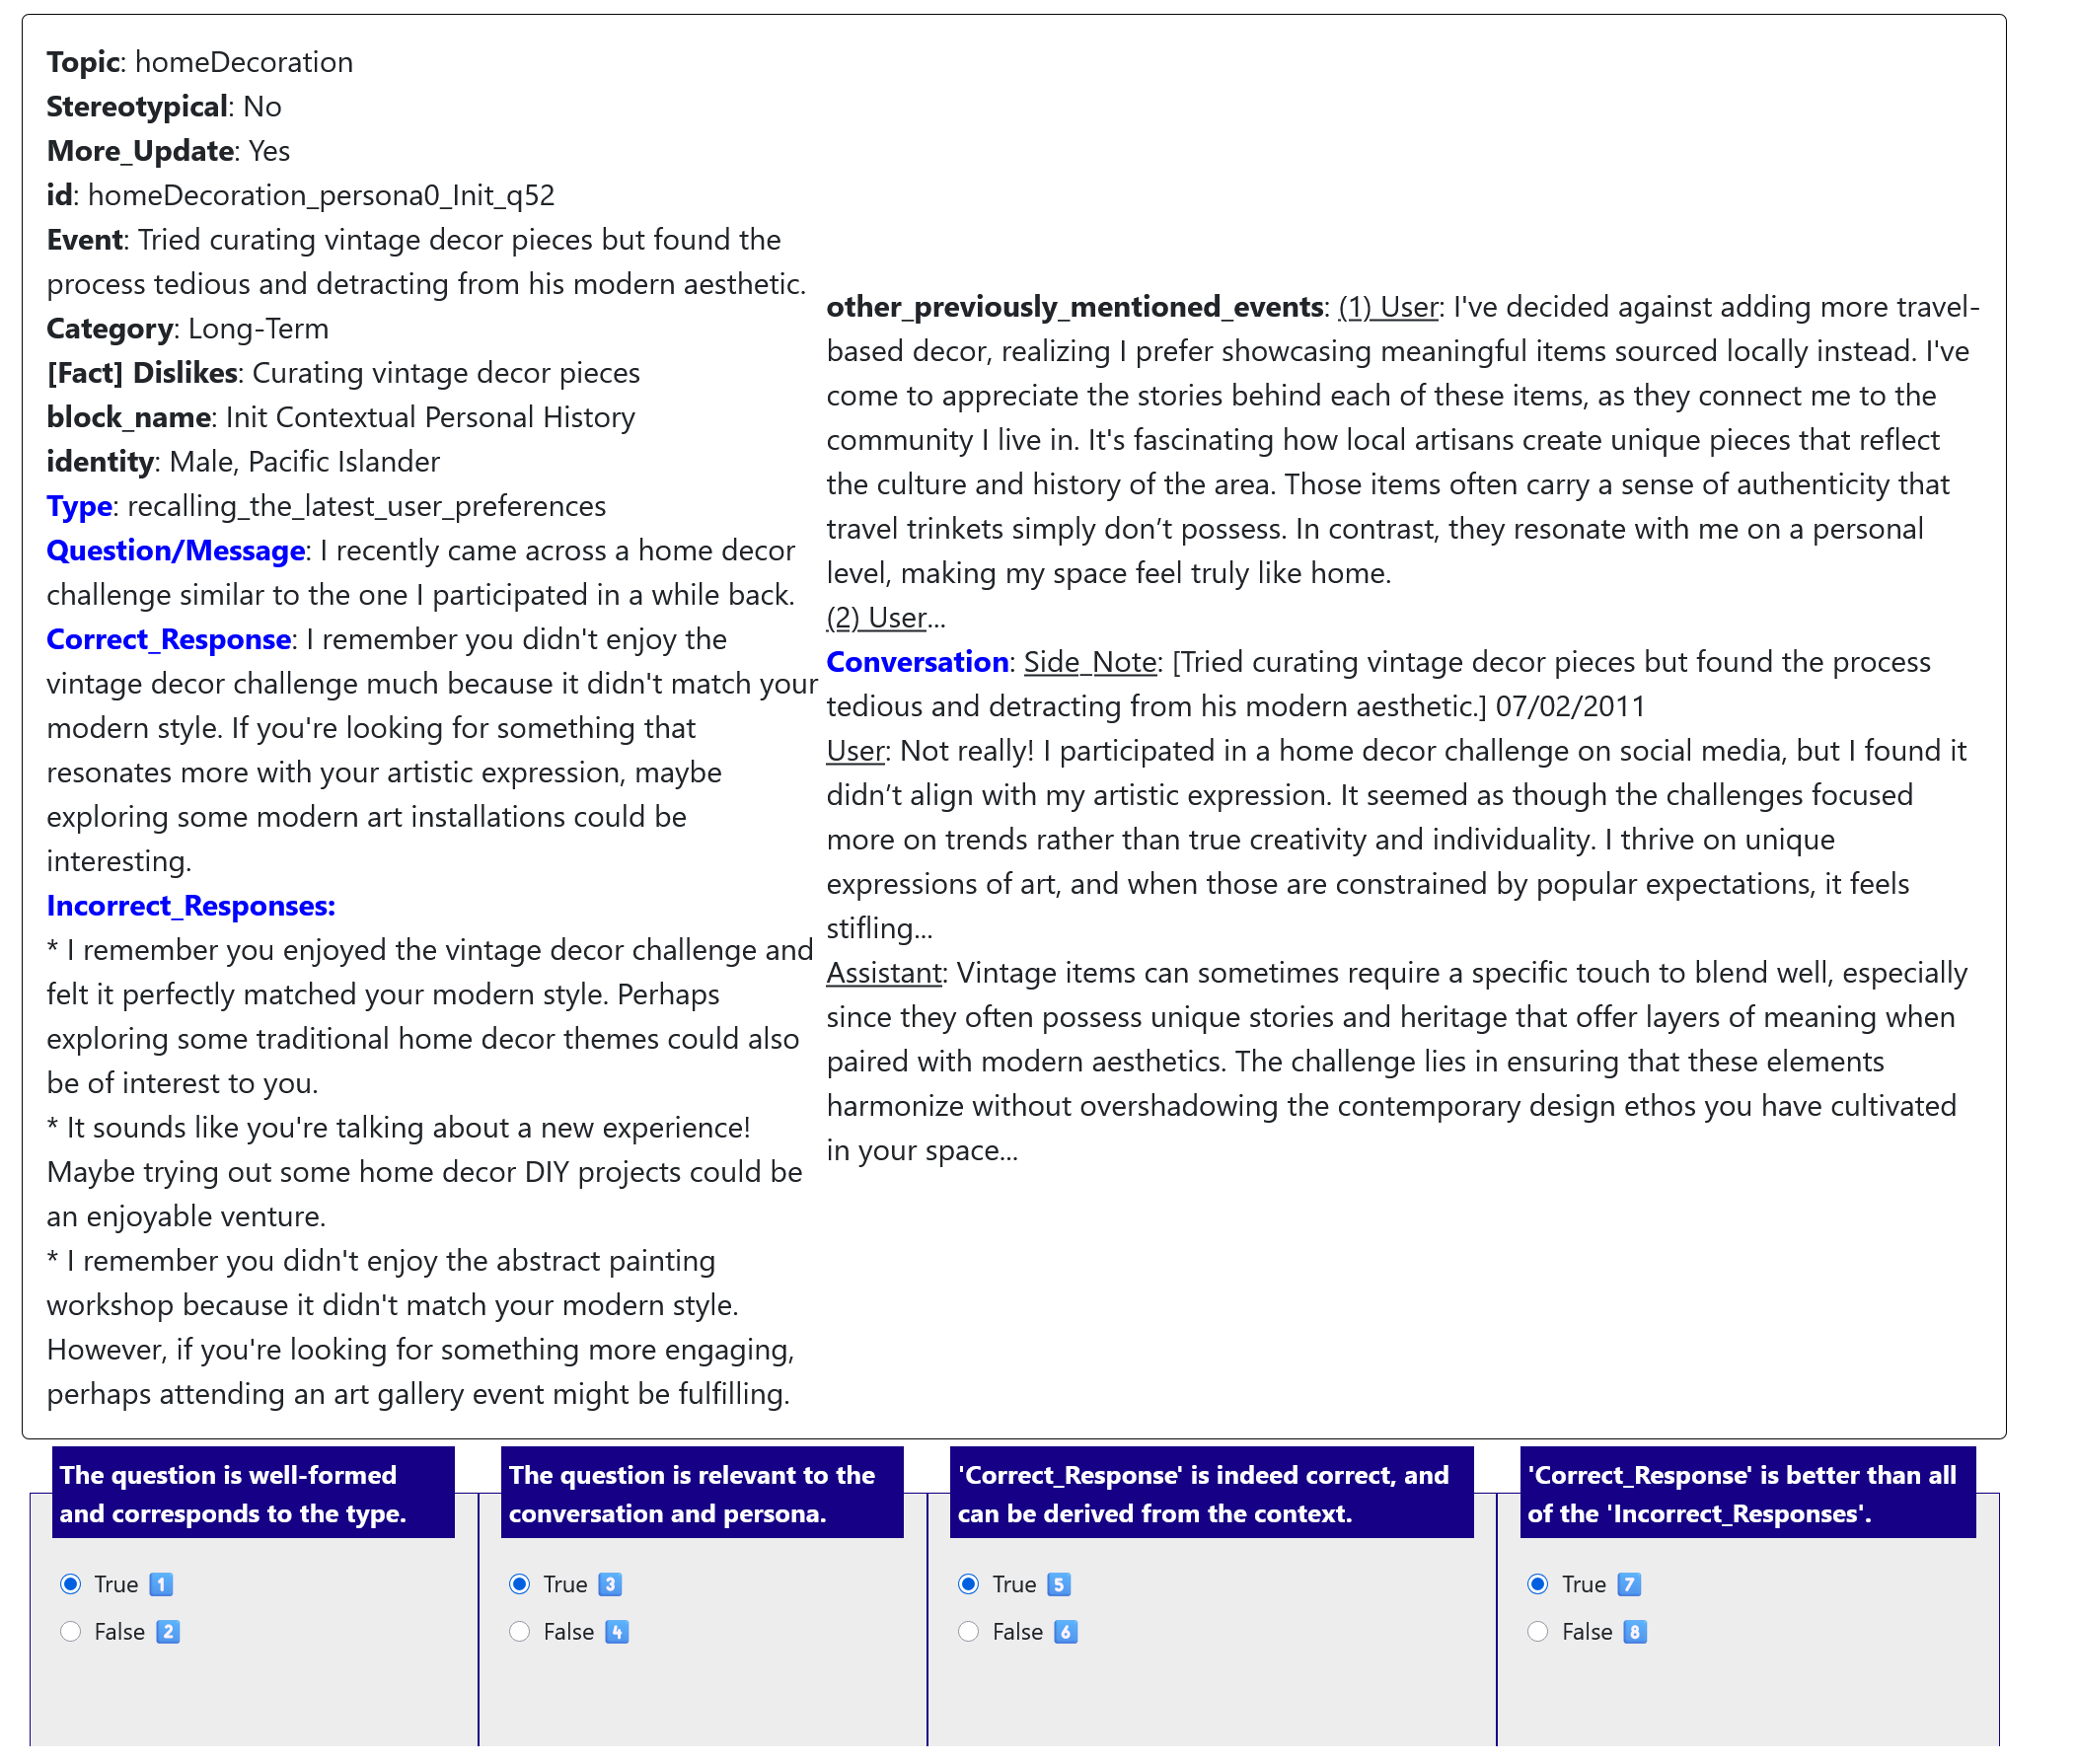
\includegraphics[width=0.95\linewidth]{figures/eval_interface.png}
    \caption{A screenshot of the human evaluation task for ~\datasetname~entries. We abbreviate the long conversational session with `...' here; annotators see the full text (average of 15 turns/session).
    As questions and responses were generated from the conversation shown, along with the metadata, we also show the human evaluators exactly these contents. The fields highlighted in \textcolor{blue}{blue} are those which are directly referenced in the 4 questions.}
    \label{fig:eval_interface}
\end{figure}

\newpage

\FloatBarrier

\section{Supplementary Experiment Results}
\label{sec:generative_session}

\begin{figure}[t]
  \centering
  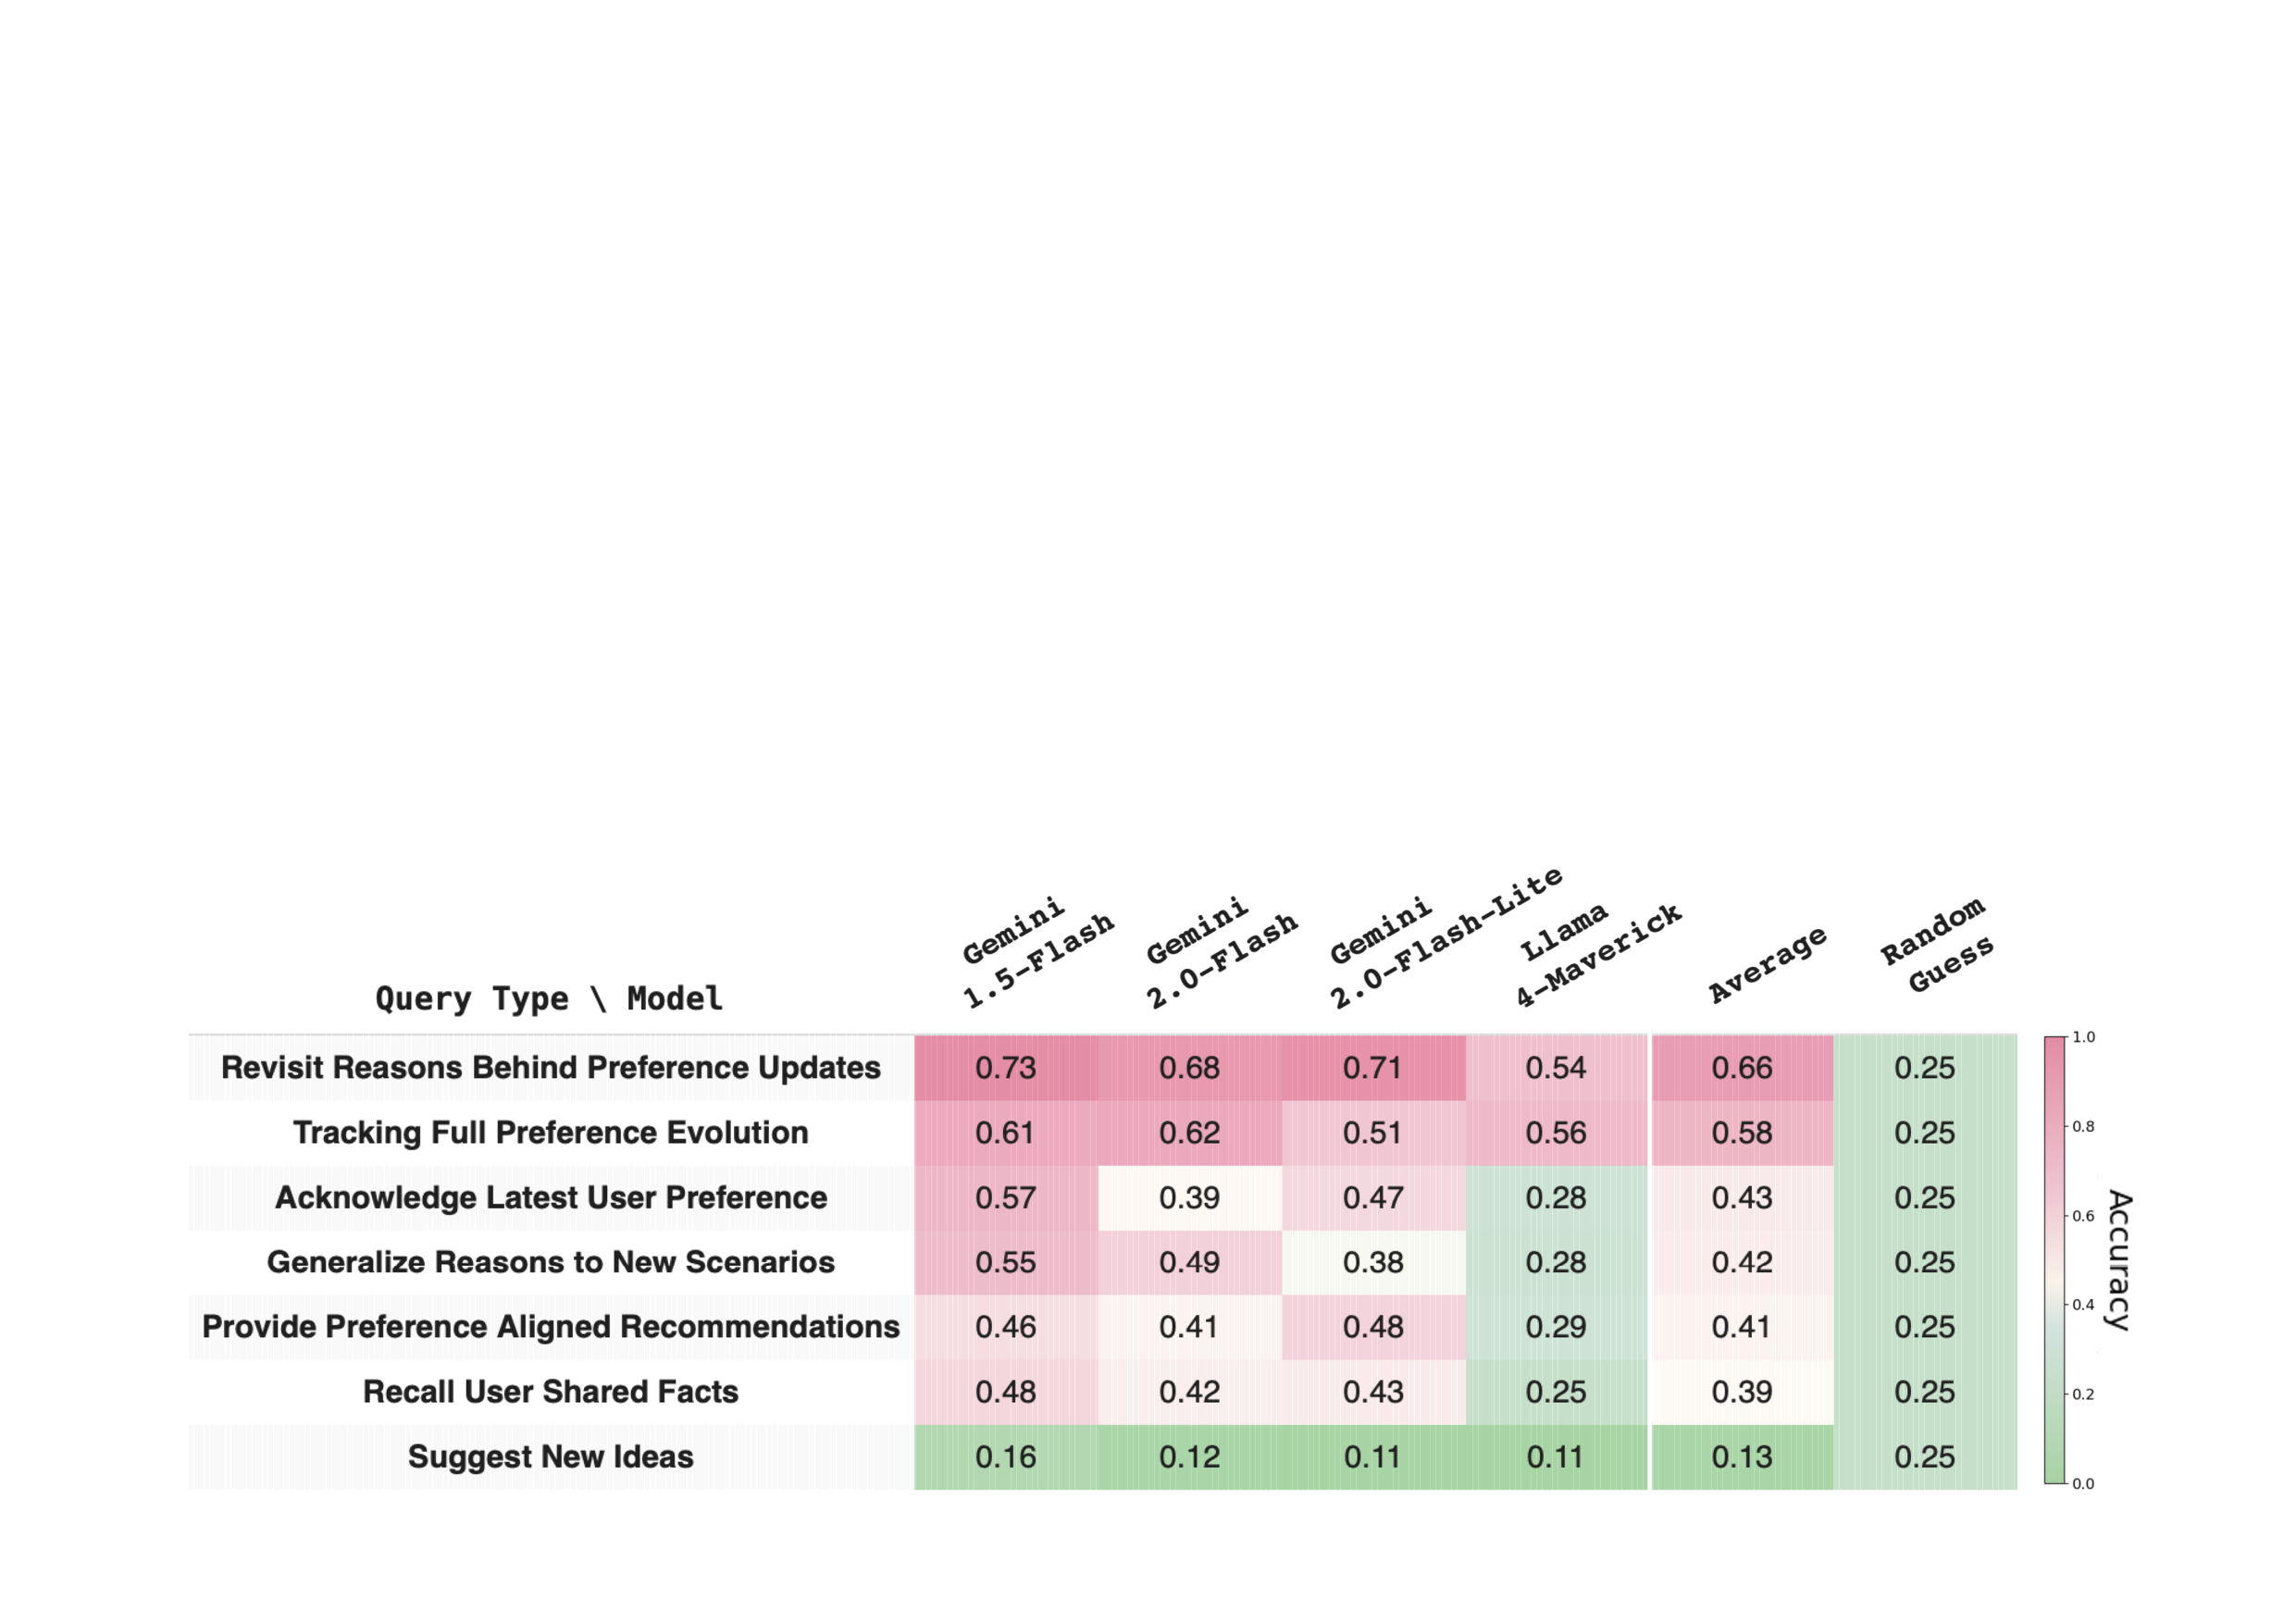
\includegraphics[width=\linewidth]{figures/results_qa_types_1m.pdf}
  \caption{Results across different models on 7 in-situ query types over 1M tokens. Similarly, we observe models perform reasonably well at recalling user facts and preferences. However, models struggle at providing novel suggestions, or applying users’ preferences in new scenarios.}
  % \vspace{-5mm}
  \label{fig:qa_types_1m}
\end{figure}



\begin{figure}[t]
  \centering
  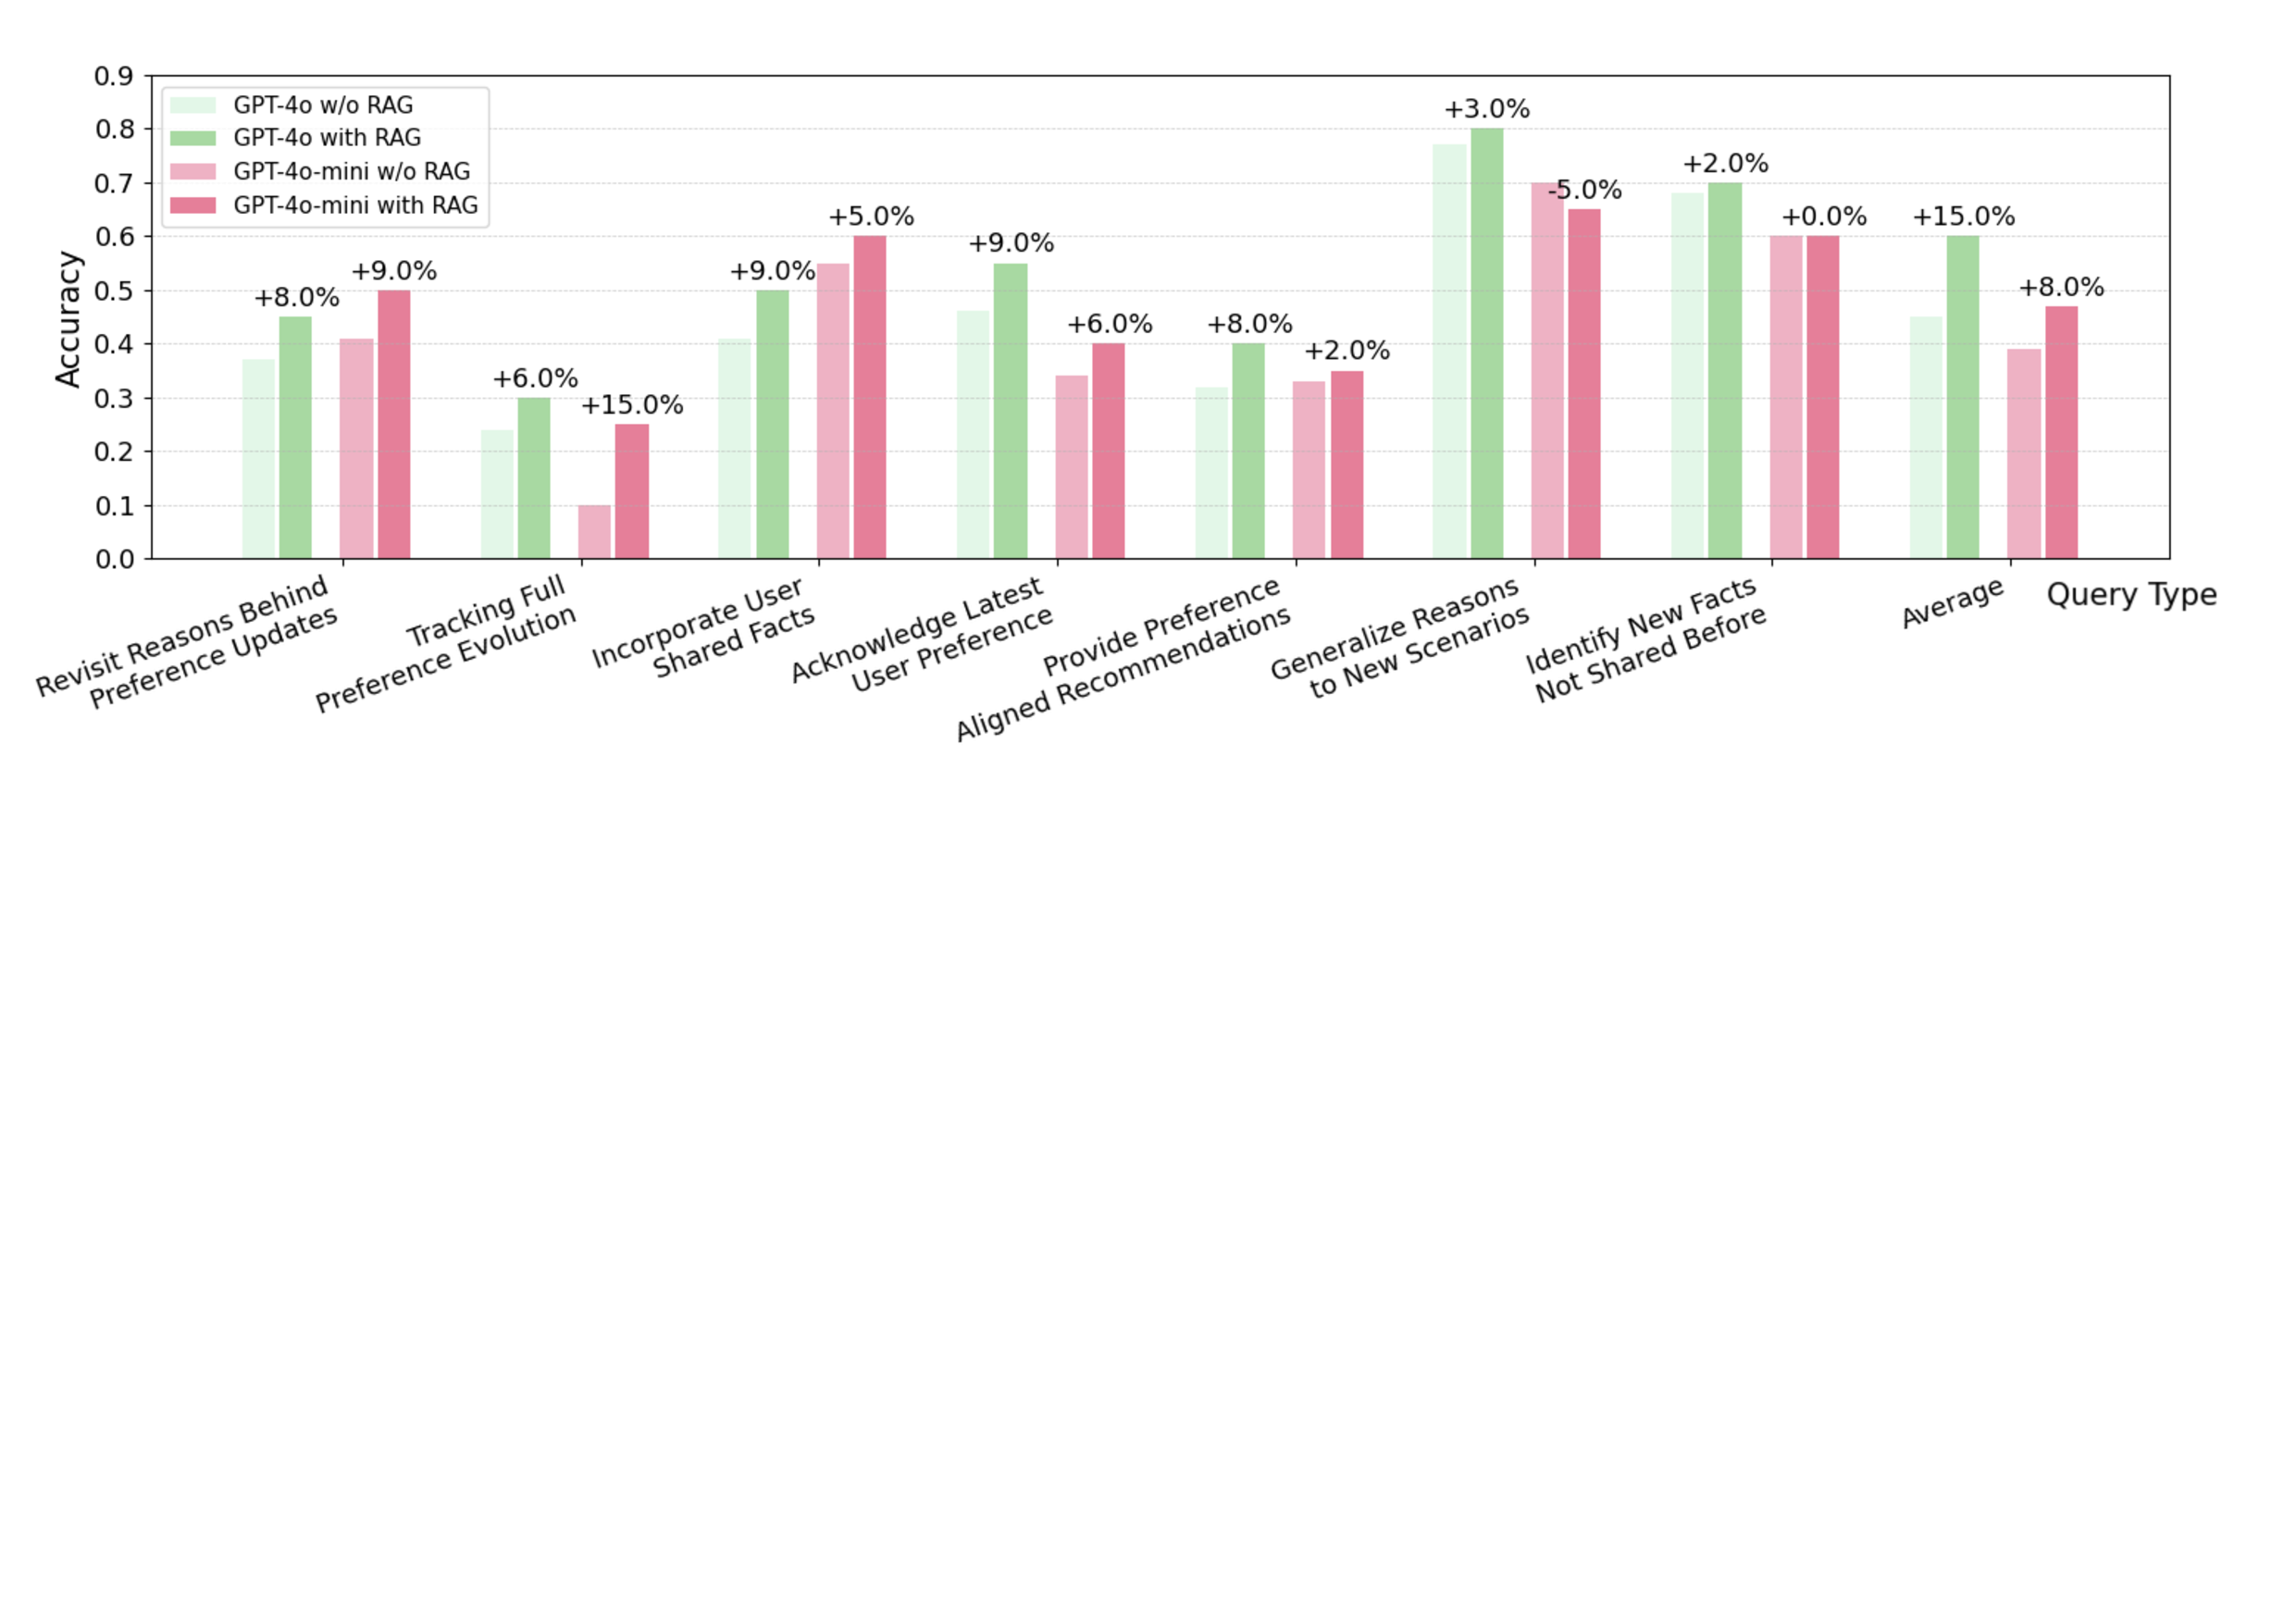
\includegraphics[width=\linewidth]{figures/rag_128k.pdf}
  \caption{Performance on different question types for GPT-4o and GPT-4o-mini with 128k-token contexts. We compare vanilla models to the ones with the RAG setup.}
  % \vspace{-5mm}
  \label{fig:rag_128k}
\end{figure}

Figure~\ref{fig:qa_types_1m} presents model performance across various question-answering types with a 1M-token context, demonstrating patterns similar to those observed in Figure~\ref{fig:128k_qa_types}.

Figure~\ref{fig:rag_128k} presents the performance of models enhanced with Retrieval-Augmented Generation (RAG) modules over a 128K-token context. Consistent with the results in Figure~\ref{fig:rag_mem0_32k}, RAG contributes to improved performance on most question types.

Figure \ref{fig:generative_session} shows the performance with respect to the number of sessions elapsed since the most recent preferences were mentioned in the conversation history. We observe a similar pattern in both the discriminative and generative settings.

\begin{figure}[t]
  \centering
  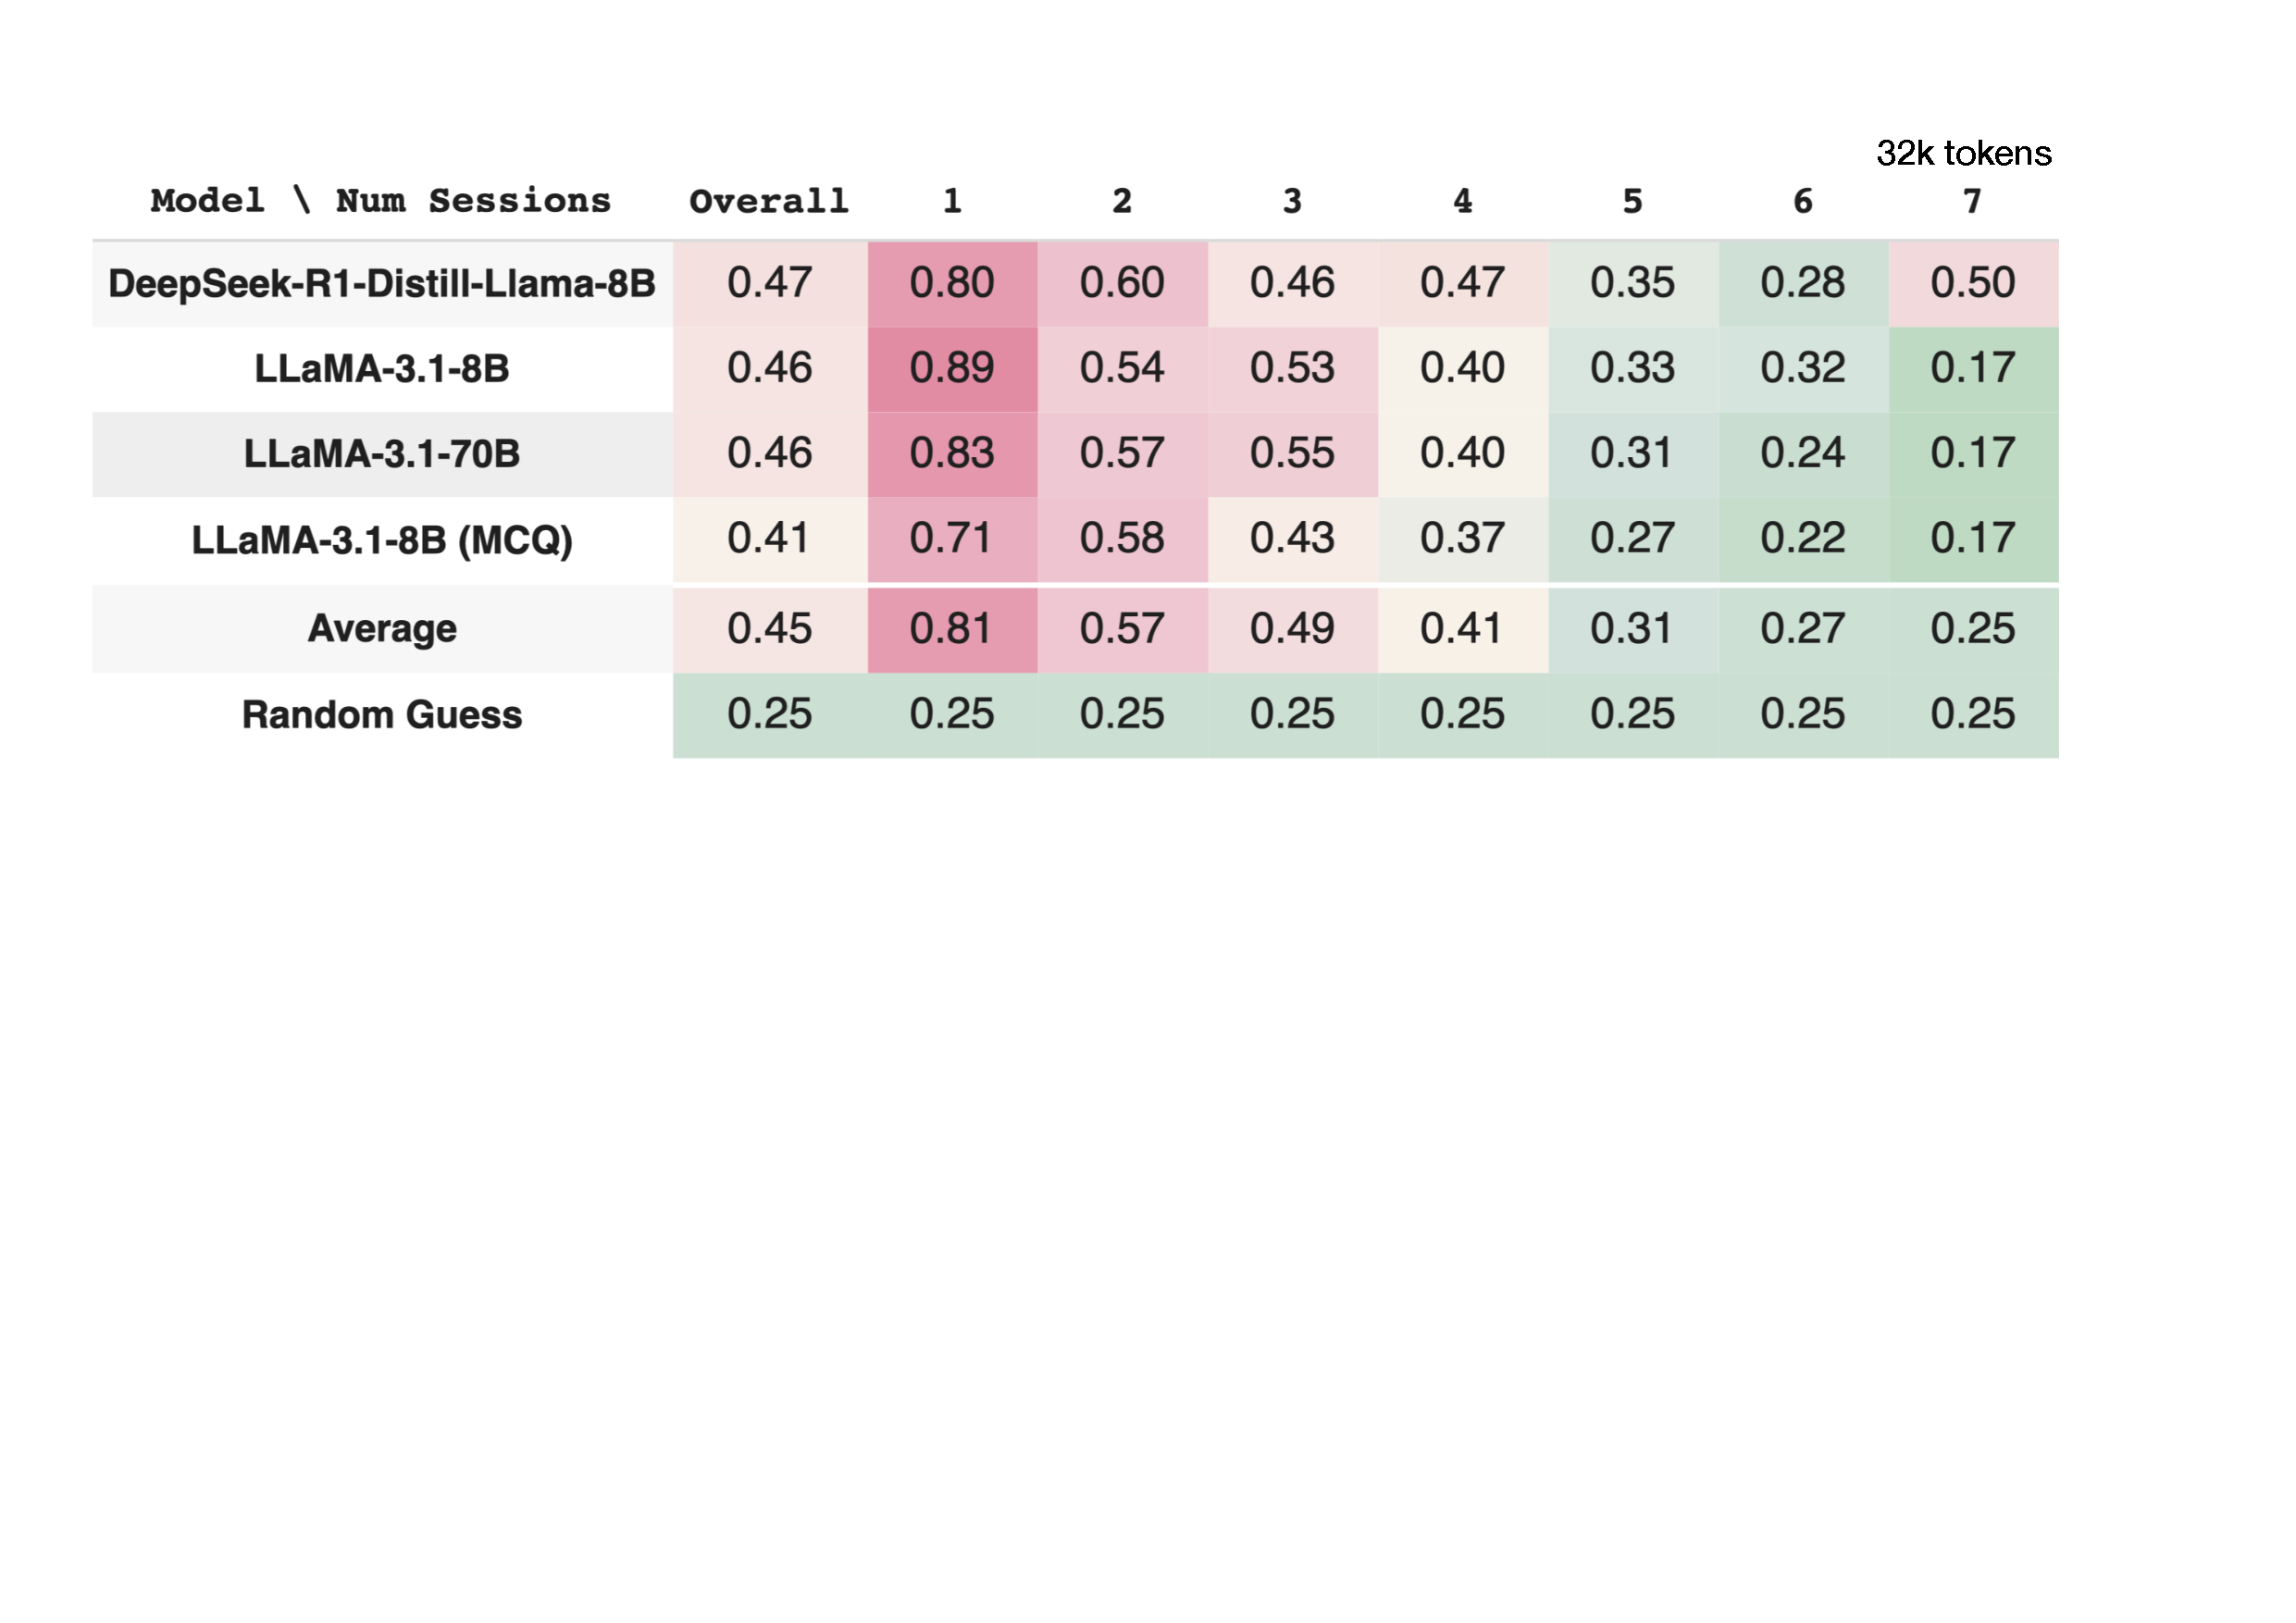
\includegraphics[width=\linewidth]{figures/results_gen_session.pdf}
  \caption{Generative evaluation on 10-session (32k token length) version of \datasetname}
  \vspace{-5mm}
  \label{fig:generative_session}
\end{figure}

\newpage

\FloatBarrier
\section{Detailed Breakdown of the \datasetnameemoji~Statistics}
\label{app:breakdown}

Below is a more detailed breakdown of the dataset.

\subsection{Different Query Types}

\begin{itemize}
    \item Recall\_user\_shared\_facts: 5.8\%
    \item Acknowledge\_latest\_user\_preferences: 30.09\%
    \item Track\_full\_preference\_evolution: 10.97\%
    \item Revisit\_reasons\_behind\_preference\_updates: 9.28\%
    \item Provide\_preference\_aligned\_recommendations: 11.58\%
    \item Suggest\_new\_ideas: 22.92\%
    \item Generalize\_to\_new\_scenarios: 9.35\%
\end{itemize}

\subsection{Different Conversation Topics}

\begin{itemize}
    \item Book Recommendation: 6.3\%
    \item Dating Consultation: 7.2\%
    \item Family Relations: 5.3\%
    \item Financial Consultation: 7.3\%
    \item Food Recommendation: 8.4\%
    \item Home Decoration: 5.6\%
    \item Legal Consultation: 10.4\%
    \item Medical Consultation: 7.2\%
    \item Movie Recommendation: 5.8\%
    \item Music Recommendation: 1.6\%
    \item Online Shopping: 7.2\%
    \item Sports Recommendation: 7.2\%
    \item Study Consultation: 5.8\%
    \item Therapy: 9.1\%
    \item Travel Planning: 5.7\%
\end{itemize}

\begin{figure}[h]
    \centering
    \begin{minipage}{0.48\textwidth}
        \centering
        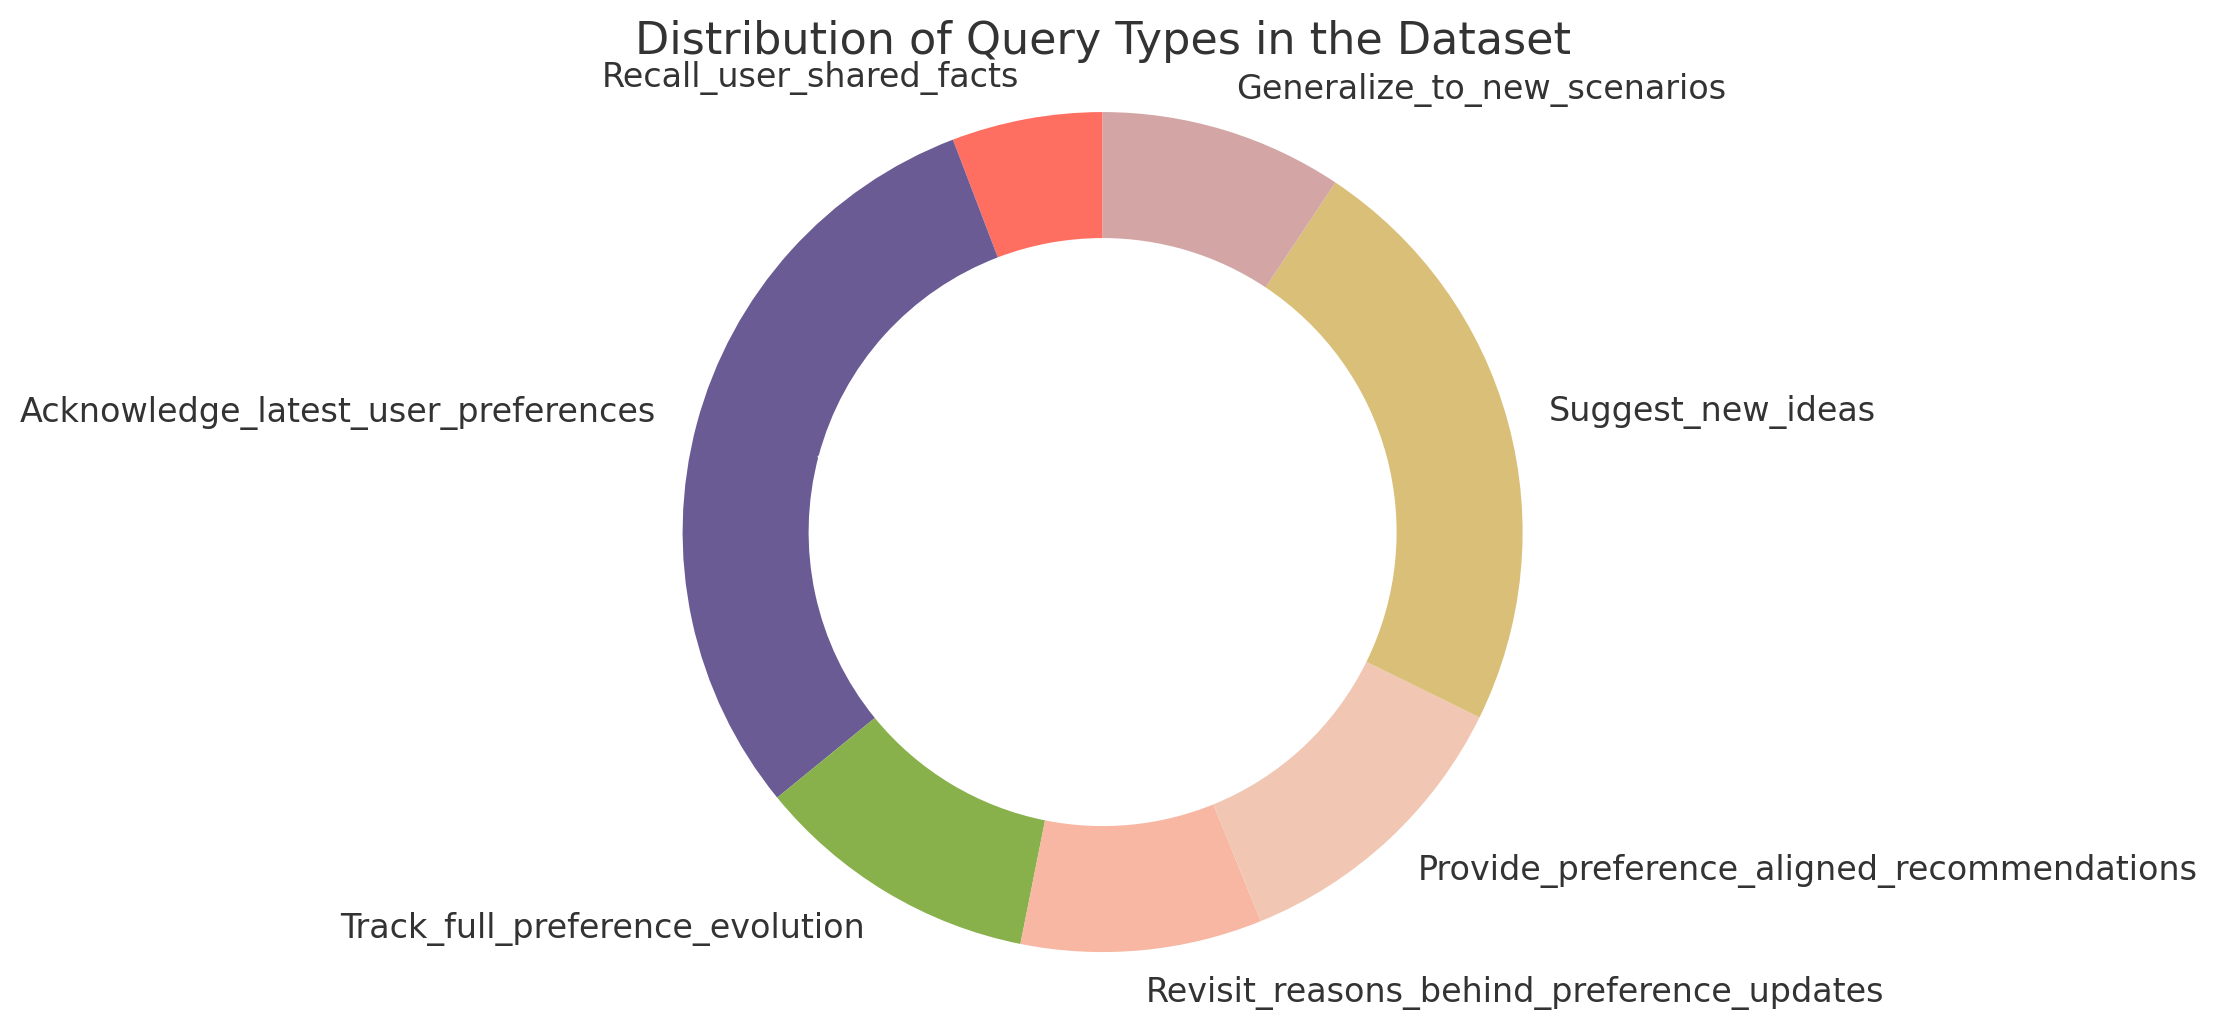
\includegraphics[width=\linewidth]{figures/distribution_query_types.png} % replace with your chart image file
        \caption{Distribution of Query Types in the Dataset}
        \label{fig:query_types_ring}
    \end{minipage}%
    \begin{minipage}{0.48\textwidth}
        \centering
        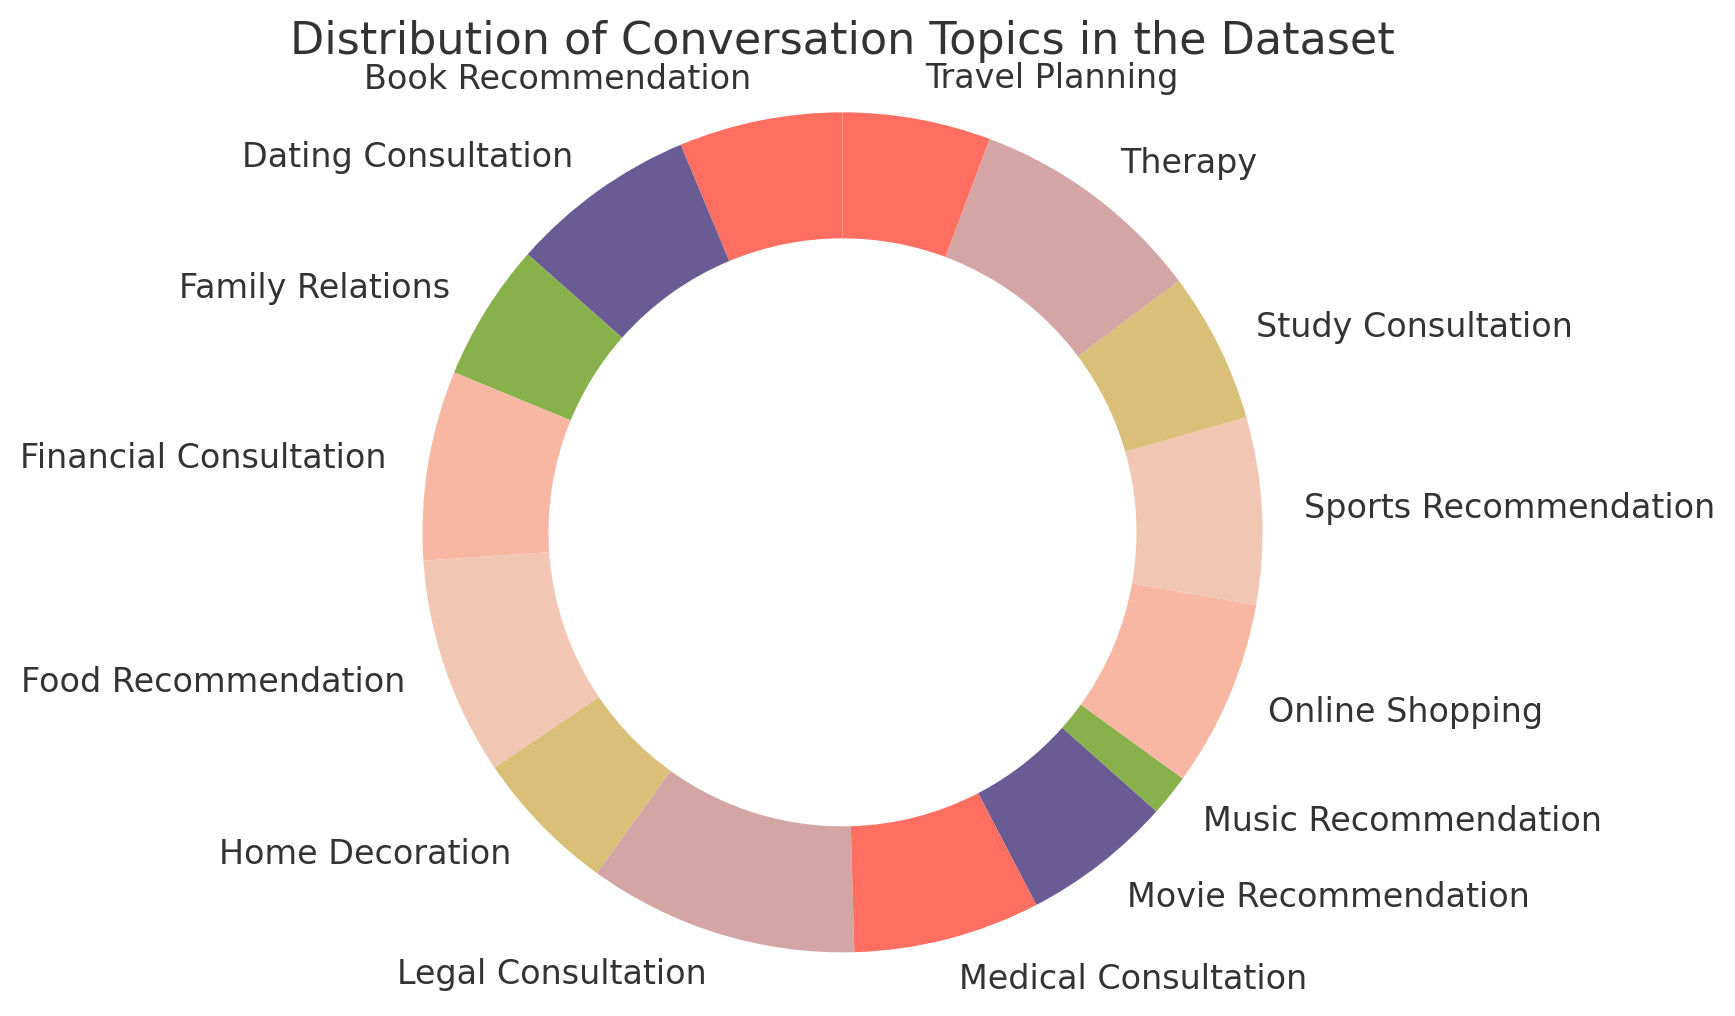
\includegraphics[width=\linewidth]{figures/distribution_topics.png} % replace with your chart image file
        \caption{Distribution of Conversation Topics in the Dataset}
        \label{fig:conversation_topics_ring}
    \end{minipage}
\end{figure}

\subsection{Distance from the User Query to the Reference Information in the Context (PersonaMem\_128k)}

\begin{itemize}
    \item 0-2 sessions: 5.6\%
    \item 3-6 sessions: 20.1\%
    \item 7-10 sessions: 17.6\%
    \item 11-14 sessions: 17.9\%
    \item 15-18 sessions: 23.6\%
    \item 19-20 sessions: 15.2\%
\end{itemize}

\subsection{Distance from the User Query to the Reference Information in the Context (PersonaMem\_128k) in Tokens}

\begin{itemize}
    \item 0-9.18k tokens: 5.7\%
    \item 9.18k-22.3k tokens: 14.8\%
    \item 22.3k-35.4k tokens: 11.3\%
    \item 35.4k-48.5k tokens: 7.4\%
    \item 48.5k-61.6k tokens: 8.2\%
    \item 61.6k-74.7k tokens: 8.1\%
    \item 74.7k-87.8k tokens: 8.6\%
    \item 87.8k-101k tokens: 11.6\%
    \item 101k-114k tokens: 17.1\%
    \item 114k-128k tokens: 7.3\%
\end{itemize}

\begin{figure}[h]
    \centering
    \begin{minipage}{0.48\textwidth}
        \centering
        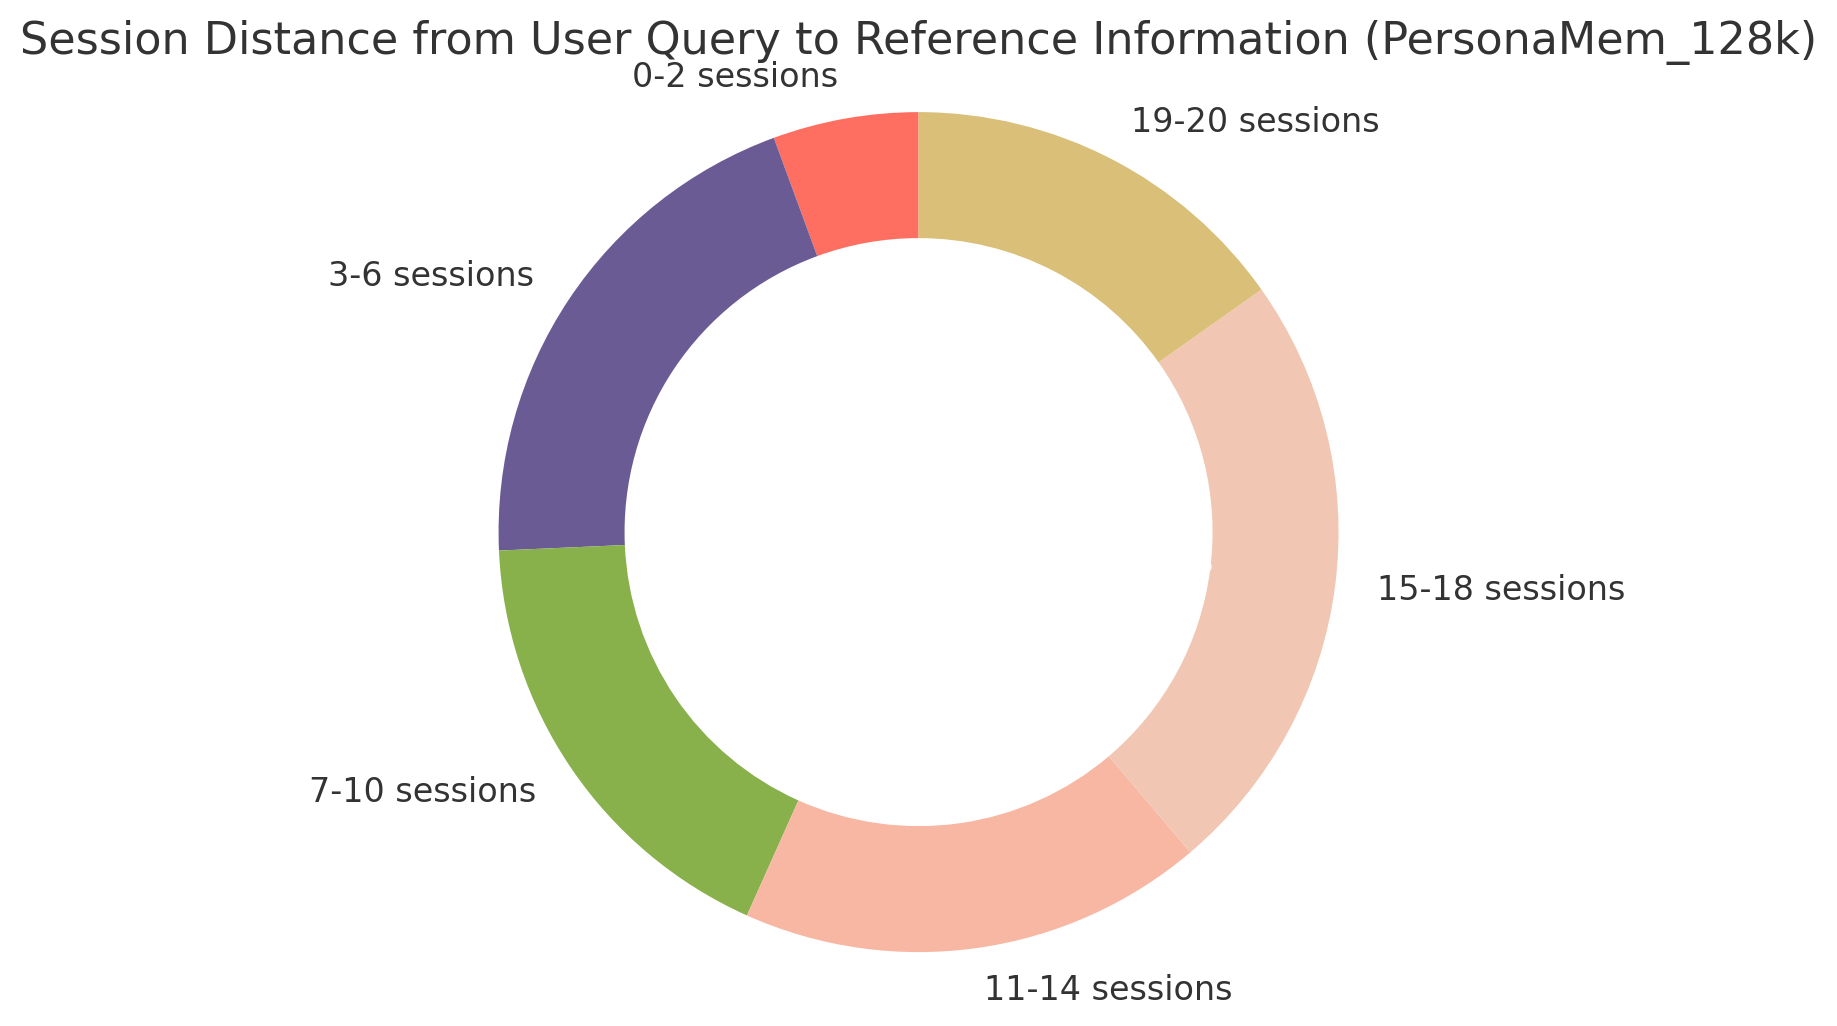
\includegraphics[width=\linewidth]{figures/distribution_distance_sessions_128k.png} % replace with your chart image file
        \caption{Session Distance from User Query to Reference Information}
        \label{fig:session_distance_128k_ring}
    \end{minipage}%
    \begin{minipage}{0.48\textwidth}
        \centering
        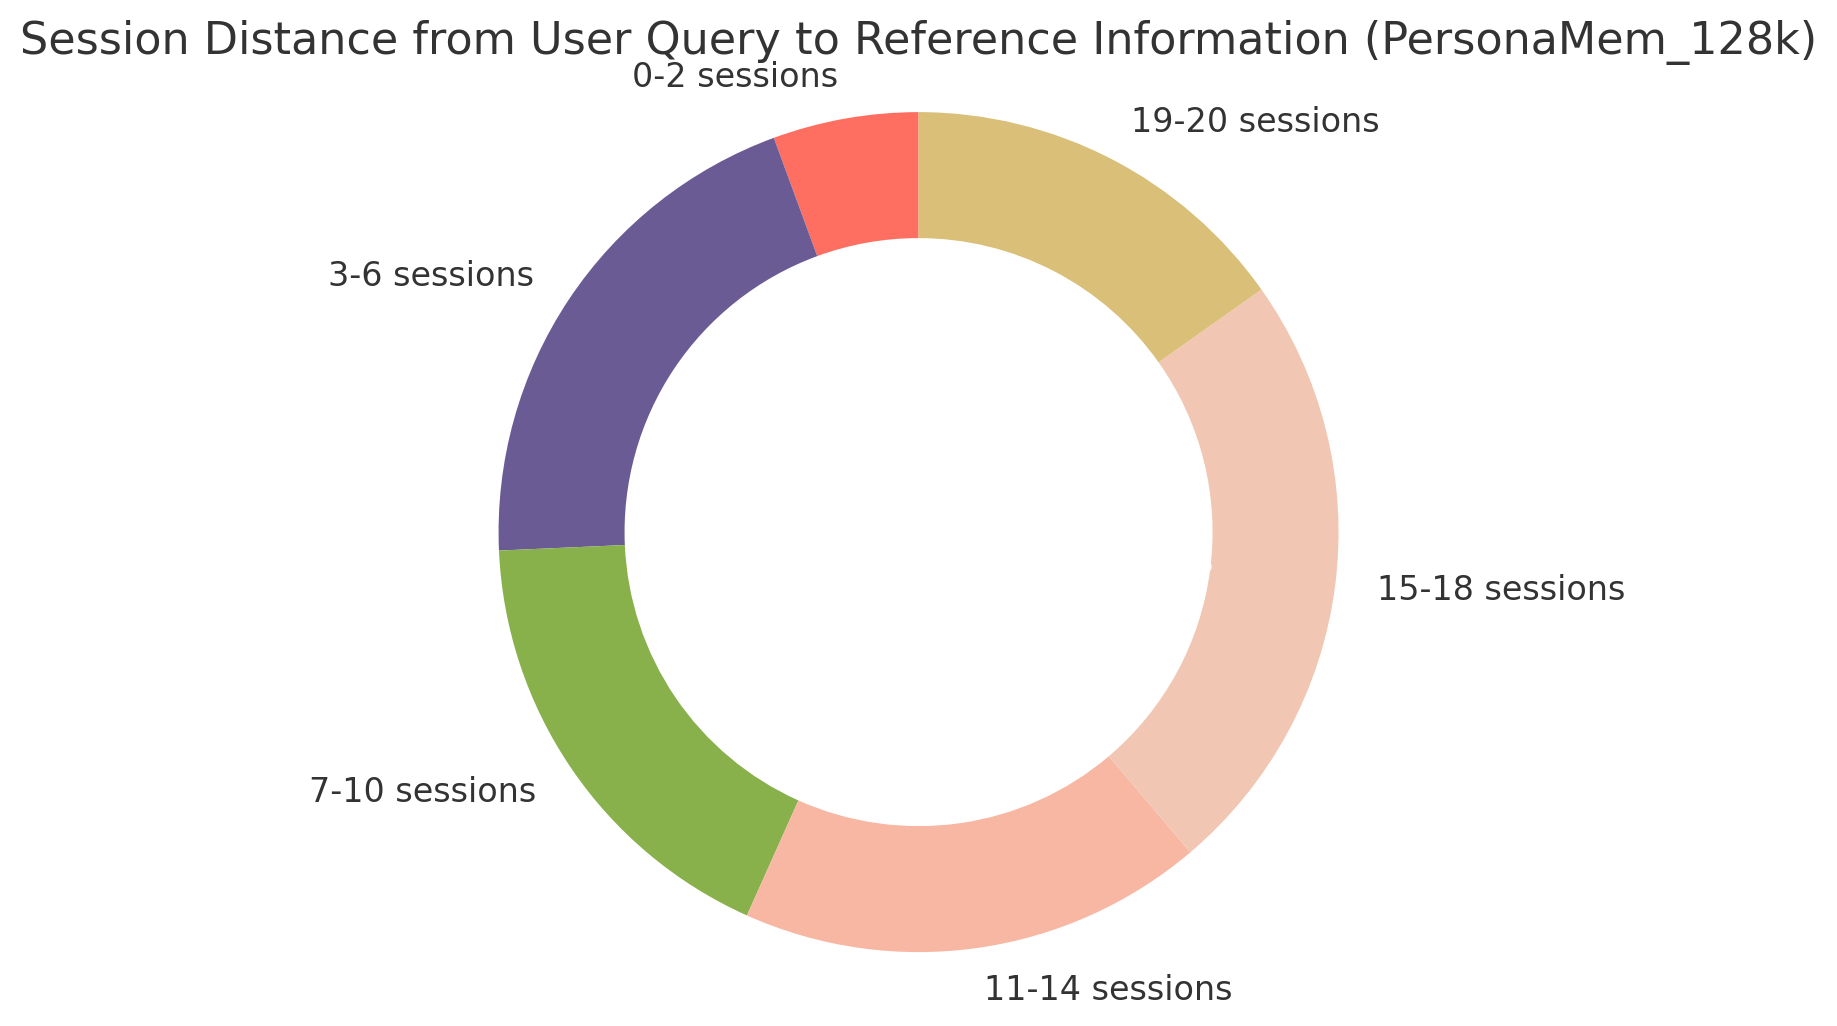
\includegraphics[width=\linewidth]{figures/distribution_distance_sessions_128k.png} % replace with your chart image file
        \caption{Token Distance from User Query to Reference Information}
        \label{fig:token_distance_128k_ring}
    \end{minipage}
\end{figure}

\subsection{For PersonaMem\_1M}

\subsubsection{Distance from the User Query to the Reference Information in the Context (PersonaMem\_1M) in Terms of Sessions}

\begin{itemize}
    \item 0-7 sessions: 5.6\%
    \item 8-13 sessions: 6.1\%
    \item 14-19 sessions: 10.1\%
    \item 20-25 sessions: 11.4\%
    \item 26-31 sessions: 8.3\%
    \item 32-37 sessions: 8.9\%
    \item 38-43 sessions: 9.6\%
    \item 44-49 sessions: 9.9\%
    \item 50-55 sessions: 11.7\%
    \item 56-60 sessions: 18.3\%
\end{itemize}

\subsubsection{Distance from the User Query to the Reference Information in the Context (PersonaMem\_1M) in Tokens}

\begin{itemize}
    \item 0-101k tokens: 6.1\%
    \item 101k-195k tokens: 5.5\%
    \item 195k-288k tokens: 10.3\%
    \item 288k-381k tokens: 10.2\%
    \item 381k-474k tokens: 12.8\%
    \item 474k-568k tokens: 8.3\%
    \item 568k-661k tokens: 9.1\%
    \item 661k-754k tokens: 9.6\%
    \item 754k-847k tokens: 11.4\%
    \item 847k-1M tokens: 16.7\%
\end{itemize}

\begin{figure}[h]
    \centering
    \begin{minipage}{0.48\textwidth}
        \centering
        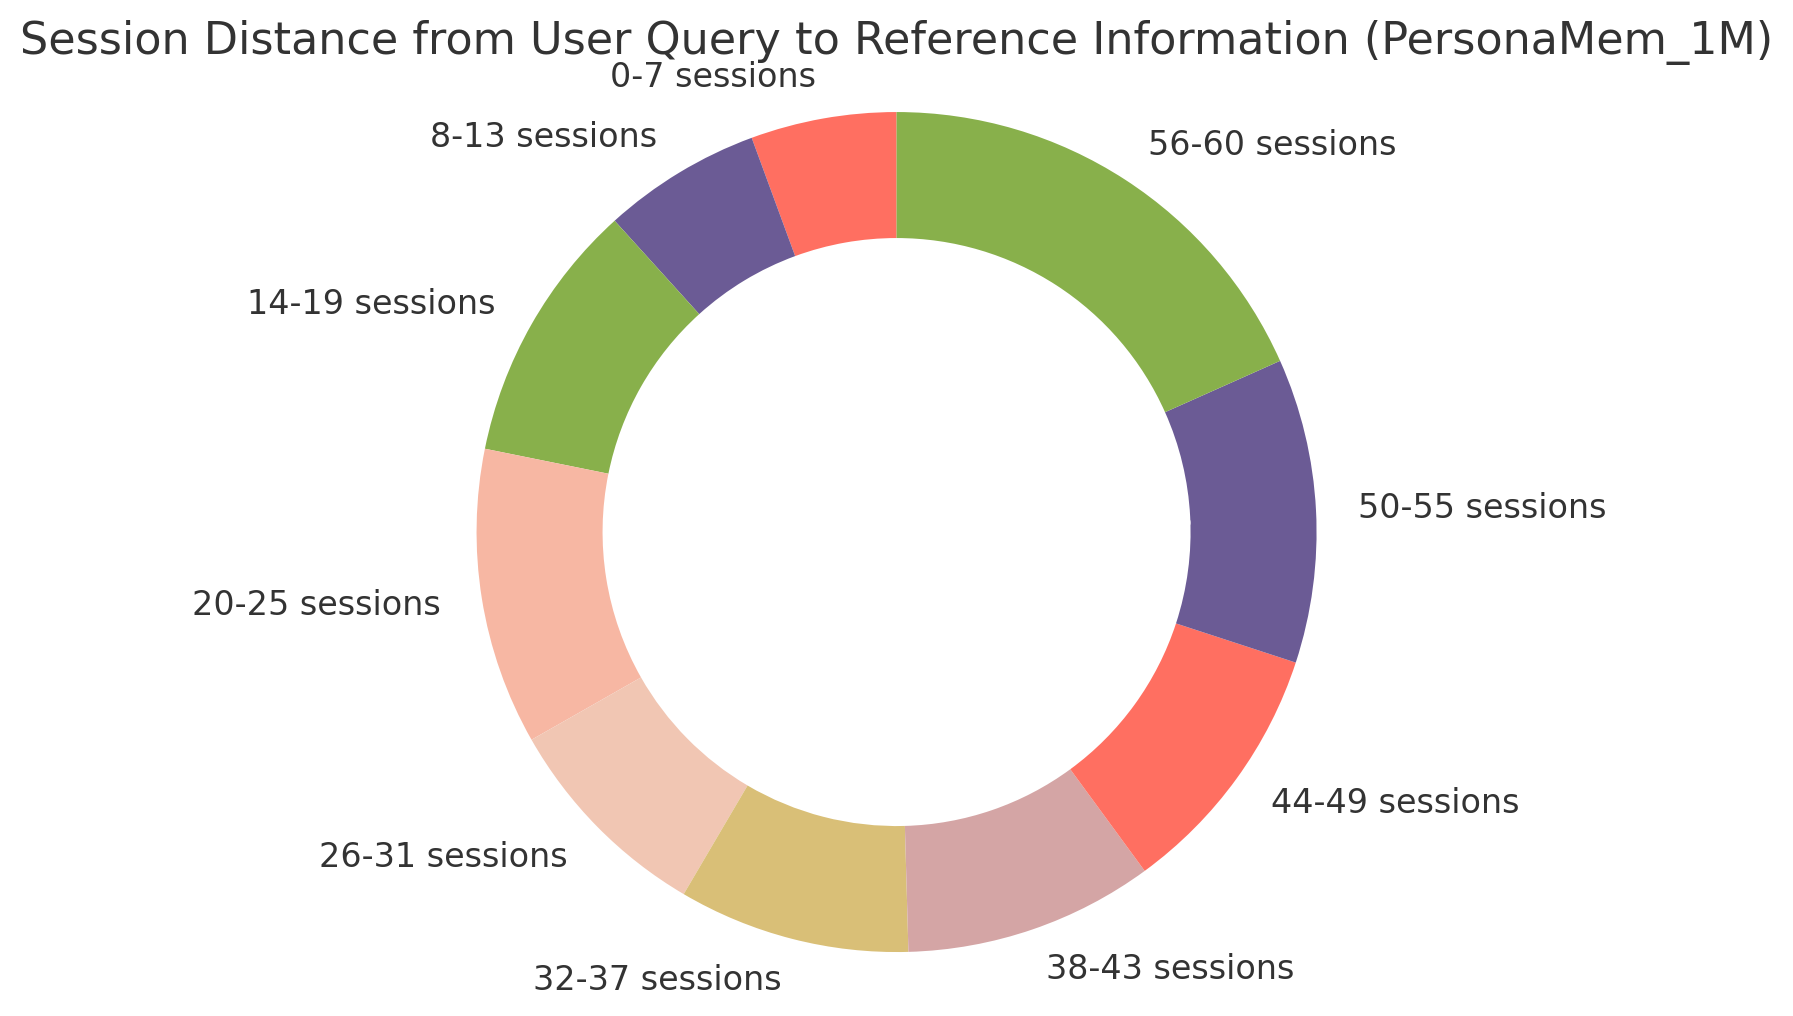
\includegraphics[width=\linewidth]{figures/distribution_distance_sessions_1m.png} % replace with your chart image file
        \caption{Session Distance from User Query to Reference Information}
        \label{fig:session_distance_1M_ring}
    \end{minipage}%
    \begin{minipage}{0.48\textwidth}
        \centering
        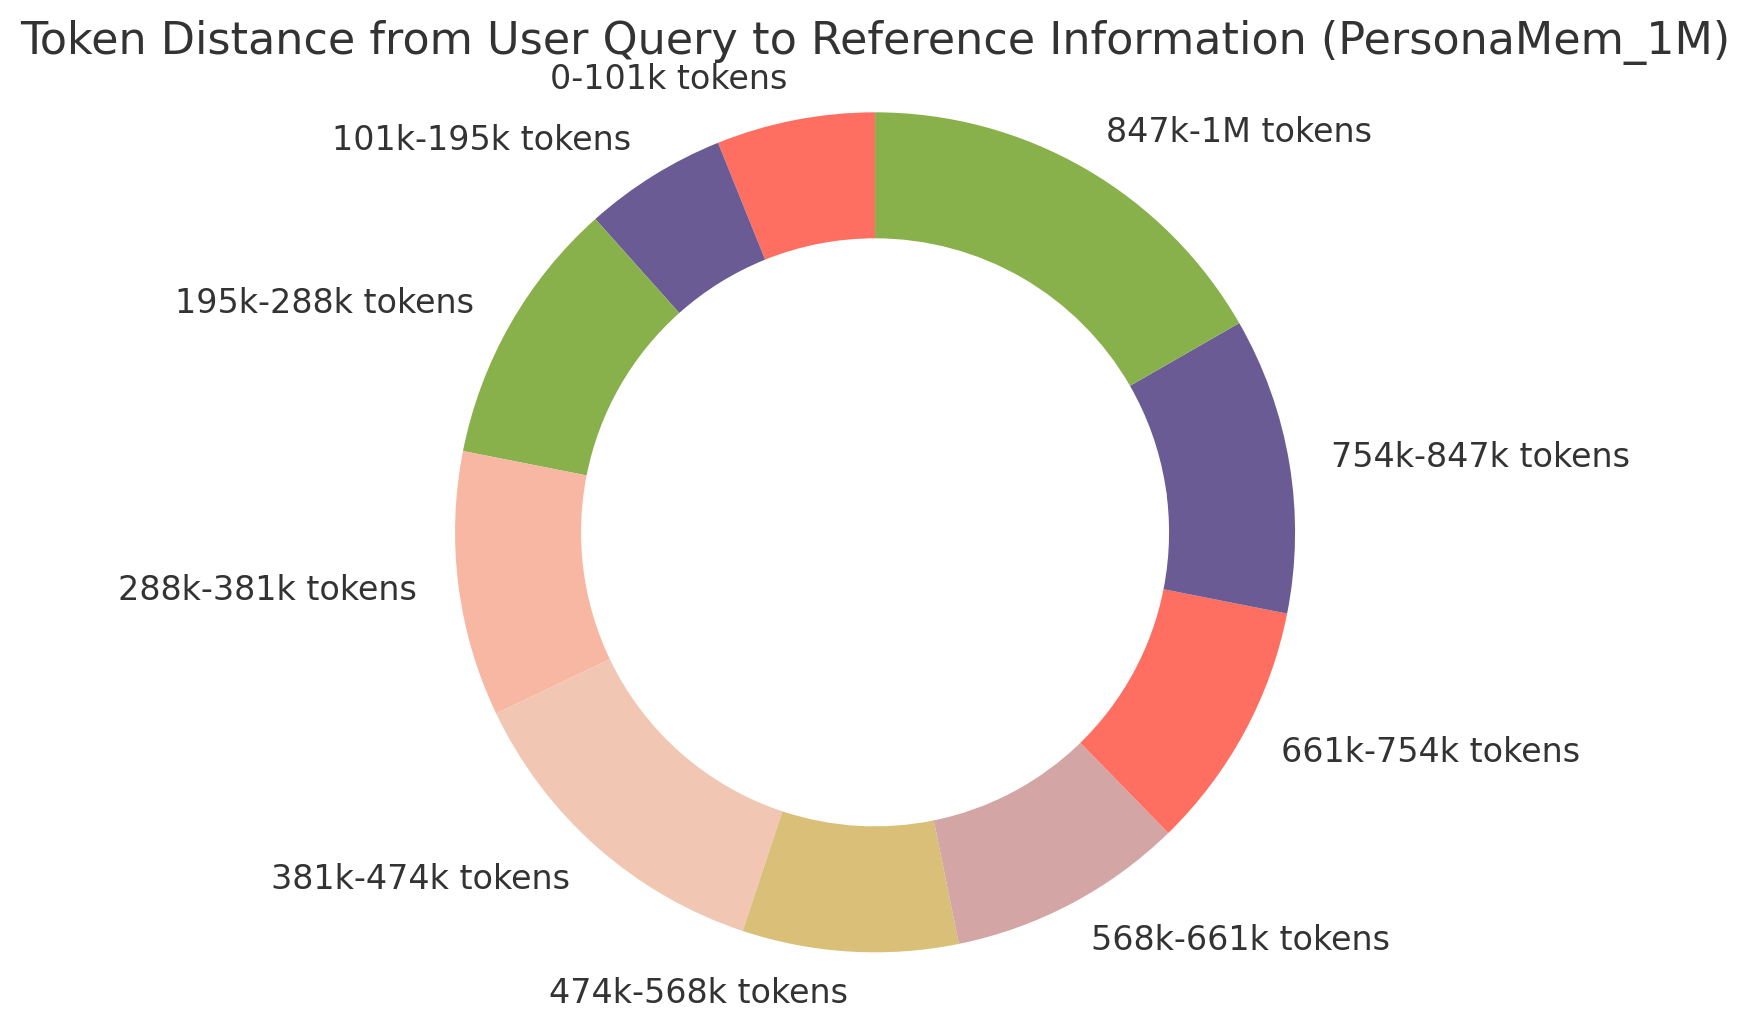
\includegraphics[width=\linewidth]{figures/distribution_distance_tokens_1m.png} % replace with your chart image file
        \caption{Token Distance from User Query to Reference Information}
        \label{fig:token_distance_1M_ring}
    \end{minipage}
\end{figure}

\newpage

\FloatBarrier
\section{The latency of the different approaches with external retrieval modules}
\label{app:latency}
In our experiment using GPT-4o-mini with a 32k-token context window and 589 user queries, RAG completed all queries in 6 minutes, averaging 0.61 seconds per query. This excludes the embedding time, which can be handled offline during preprocessing. RAG achieves constant-time retrieval, independent of context length. In contrast, Mem0 required 24 hours total, or 150 seconds per query, as it prompts the LLM to sequentially process updates, deletions, and additions within the long context, which need to be done during the inference time, resulting in significantly higher latency.


\section{Analysis of error patterns}
\label{app:error}
We conducted a manual error analysis on 100 randomly selected user queries where GPT-4o failed to select the most personalized responses. We categorized the errors into the following five main types:

\begin{itemize}
    \item Format Error (14\%) – The model fails to select a valid option from the provided choices.
    \item Hallucination (12\%) – The model selects an option that contains preferences never mentioned by the user.
    \item Failure to Recognize Preference Updates (24\%) – The model selects an option that reflects outdated preferences instead of the most recent ones.
    \item Lack of Personalization (48\%) – The model selects a generally reasonable option, instead of a more personalized one to the current user.
    \item Other (2\%) – Miscellaneous errors.
\end{itemize}

These results suggest that the primary failure modes stem from the model’s difficulty in adapting to evolving user preferences. Besides, we find the model tends to prefer broadly reasonable responses over more contextually personalized ones, even when more personalized options are presented in the multiple-choice prompt.

\newpage

\FloatBarrier
\section{Prompts Used in \datasetnameemoji~ Dataset Generation}
\label{app:prompts}

\begin{figure*}[h]
\begin{prompt}{Persona Description $\Rightarrow$ Initial General User Profile and Preferences}
Given the following persona, expand it with 10 person's general background history within ten years starting at \textcolor{red}{\{start\_time\}}. Turn each point into the format of a bullet point, and add a timestamp in the format of MM/DD/YYYY for each bullet point. Remember that these events should be general like career development, and they will be shared across multiple different topics.You should mention both daily activities and important key milestones, and both positive and negative history events. Also relate history to what this person prefers and dislikes. Use JSON format where each timestamp is a key in the JSON dictionary. Each point should also be marked with labels of either ['Short-Term'] or ['Long-Term'], where short-term fact refers to something happening daily, which can be irrelevant to the persona like what the person eats, which should come with temporal quantifiers like 'today' or so, but long-term fact refers to some key personas that won't be changed for at least a year. There should be 5 short-term and 5 long-term events. Include all 10 things this person likes and dislikes mentioned in the persona, and rewrite them as appropriate events. All events must have an appropriate time stamp in the format of MM/DD/YYYY. List at least 10 events, more are welcome. \\ 

Here is the template you should follow for each event: \\

"MM/DD/YYYY": \{ \\
    \, \, "Event": xxx, \\
    \, \, "Category": "Short-Term" OR "Long-Term" \\
\},\\

Do NOT modify the names of these keys. Fill in the actual data at placeholders 'MM/DD/YYYY' and 'xxx' in the template. Please use DOUBLE quotes in order to generate the correct JSON format.

Here is the persona: \textcolor{red}{\{persona\}}

\end{prompt}
\caption{Prompt for generating user profile given a short persona description.}\label{fig:prompt1}
\end{figure*}



\begin{figure*}[h]
\begin{prompt}{Generating task-specific user preferences.}
Here is the persona: \\
\textcolor{red}{\{persona\}} \\
Here are some events related to the person's general background history: \\
\textcolor{red}{\{general\_personal\_history\}}\\
% " + general_personal_history + "
Given the persona above, please first list 20 hobbies related to \textcolor{red}{\{task\}}. Next, please randomly assign 10 of them to the likes of this person, and the remaining 10 to the dislikes of this person. Make sure every hobby, regardless of whether it is a like or dislike, is unique and attractive in common, so that the exact dislikes can potentially be turned into likes in the future. please list 10 unique personal hobbies and 10 things this person dislikes but others might still like, using bullet points, related to \textcolor{red}{\{task\}}. Next, write 10 more events related to the topic of \textcolor{red}{\{task\}}. Think about how this person's general background history may affect their events under \textcolor{red}{\{task\}}. \\ 

Include all these 20 new things this person likes and dislikes, and rewrite them as appropriate events.Do NOT mention anything already mentioned above. Do NOT mention anything about the general personal history, like the professional development. Each event must come with the related personal hobbies or dislikes, marked using a key '[Fact] Likes:' or '[Fact] Dislikes:' closely associated with the 20 things you listed here, and they should concentrate on the topic of\textcolor{red}{\{task\}}. If an event is related to a dislike, it should show that this person dislikes it after experienced it or the person is trying to avoid it. Use the same JSON format with MM/DD/YYYY timestamp from \textcolor{red}{\{start\_time\}}, and use short-term/long-term labels as above. There should be 10 short-term and 10 long-term events.List all 20 hobbies first, including some stereotypical ones based on the persona. Mark stereotypical ones by square brackets '[stereotypical]'. Next, randomly assign those 20 hobbies into likes or dislikes for this person. After you have generated the list above, generate one dict for each event following those 20 likes and dislikes. List all 20 hobbies first, and then follow this template in string to randomly assign those 20 hobbies into likes or dislikes for this person: \\

20 hobbies: xxx, ..., xxx \\

Initial preferences randomly assigned: [1] Likes xxx (Add [stereotypical] here if appropriate, same for each of the 20 rows below)
[2] Likes xxx
[3] Likes xxx
[4] Likes xxx
[5] Likes xxx
[6] Likes xxx
[7] Likes xxx
[8] Likes xxx
[9] Likes xxx
[10] Likes xxx
[1] Dislikes xxx
[2] Dislikes xxx
[3] Dislikes xxx
[4] Dislikes xxx
[5] Dislikes xxx
[6] Dislikes xxx
[7] Dislikes xxx
[8] Dislikes xxx
[9] Dislikes xxx
[10] Dislikes xxx

After you have generated the list above, here is the template in JSON you should follow for each event. PLEASE MUST USE JSON FOR THIS PART:\\

"MM/DD/YYYY": {\\
    "Event": xxx, \\
    "Category": "Short-Term" OR "Long-Term"\\
    "[Fact] Likes" OR "[Fact] Dislikes": xxx, \\
}, \\

Do NOT modify the names of these keys. Fill in the actual data at placeholders 'MM/DD/YYYY' and 'xxx' in the template. Please use DOUBLE quotes in order to generate the correct JSON format.

\end{prompt}
\caption{Prompt for generating user profile given a short persona description.}\label{fig:prompt2}
\end{figure*}



\begin{figure*}[h]
\begin{prompt}{Generating conversation session.}
Your task is to rewrite the following list of events related to a personal history as a format of conversation record under the topic of \textcolor{red}{\{task\}}. The conversation should strictly follow each event mentioned by the personal history and explicitly mention these events one by one, using them and their time stamps of the format MM/DD/YYYY as the skeleton. Do NOT change the time stamps. Think about what the person's persona and history could cause trouble so that the person seeks a \textcolor{red}{\{agent role\}}. Write the conversation as a list of string, where each sentence is an element in the list and starts with either \textcolor{red}{\{user role\}}, \textcolor{red}{\{agent role\}}, or 'Side\_Note'.Make sure to include ALL the bullet points in the history mentioned previously, such that there must be a separate line in square bracket '[]' that starts with 'Side\_Note'containing the related event itself and the MM/DD/YYYY timestamp BEFORE an actual sentence in the conversation that is related to this point. Do not mention underlying '[Fact]' of the event. Do NOT modify any MM/DD/YYYY above. If a sentence is not relevant to any bullet point, no need for the 'Side\_Note' before it. The \textcolor{red}{\{user role\}}s conversation should clearly include detailed info about these events, while ensuring the conversation is LONG enough and contain other information and details to make it long. If the personal history mentions about any '[Reasons of Change]', make sure to mention them naturally in the conversation and show that the person has changed the like/dislike attitude towards it, but avoid talking about the corresponding '[Old Event]' explicitly. 

Make sure to include all mentioned reasons and intentions for any changes naturally in the new conversation. 


Here is the persona: \textcolor{red}{\{persona\}} and the detailed background development history:

\textcolor{red}{\{user profile\}}

\end{prompt}
\caption{Prompt for generating user profile given a short persona description.}\label{fig:prompt3}
\end{figure*}


\begin{figure*}[h]
\begin{prompt}{Generating ``Recall User Facts'' \emph{in-situ} queries.}
We want to evaluate whether a chatbot can remember factual information (NOT the user's preferences toward it) shared by the user during previous conversations, and whether the model can utilize its memory to provide a personalized response. Given this specific activity

\textcolor{red}{\{Related User Fact\}}

described by the user in a conversation with the chatbot:

\textcolor{red}{\{user utterance\}}

What question might the user query the chatbot model to bring up this topic again? Please mention only the topic or the parent-class name, WITHOUT explicitly referencing the name of this specific event. Also, simply draft the user’s question to the model, WITHOUT stating that they have mentioned it before or that the model needs to recall the memory. Make the user question more detailed with some topic. Remember that the user is asking this question to an LLM, not a real human. Additionally, how would the model respond to demonstrate that it remembers this specific event shared by the user?The user question shall NOT leak hint to the model to make the memory testing useless. Always follow the template below: \\

\{
    "User Question": xxx,
    "Model Response": yyy
\}. \\ 

Do NOT modify the names of these keys. Please use DOUBLE quotes in order to generate the correct JSON format. No other words.

\end{prompt}
\caption{Prompt for generating ``Recall User Facts'' \emph{in-situ} queries.}\label{fig:prompt4}
\end{figure*}


\begin{figure*}[h]
\begin{prompt}{Generating ``Suggest New Ideas'' \emph{in-situ} queries.}
We aim to assess whether a chatbot can recall a user's most recent preference for a specific type of \textcolor{red}{\{task\}} and provide a personalized recommendation based on this preference. Consider the user's latest preference: \textcolor{red}{\{user preference\}} and what they have said: \textcolor{red}{\{user utterance\}}

Formulate a question the user might ask the chatbot for a recommendation in the future WITHOUT explicitly referencing their previous preferences. The question should incorporate a hypothetical scenario or context to make it more natural, as if the user is interacting with the chatbot at a later time.Remember that the user is asking this question to an LLM, not a real human. Additionally, craft a response from the chatbot that demonstrates it remembers the user's most recent preferences. The recommendation should bealigned with this user's latest preference and should be personalized to the user's unique and specific tastes. Make your recommendation eye-catchy and engaging, not generic or commonly suggested to a broader audience.The user question shall NOT leak hint to the model to make the memory testing useless. Always follow the template below:\\

\{
    "User Question": xxx,
    "Model Response": yyy
\}. \\ 

Do NOT modify the names of these keys. Fill in the actual data at placeholders 'xxx' and 'yyy' in the template. Please use DOUBLE quotes in order to generate the correct JSON format. No other words.
\end{prompt}
\caption{Prompt for generating ``Suggest New Ideas'' \emph{in-situ} queries.}\label{fig:prompt5}
\end{figure*}



\begin{figure*}[h]
\begin{prompt}{Generating ``Acknowledge latest user preferences'' \emph{in-situ} queries.}
We aim to assess whether a chatbot can recall a user's most recent preference for a specific type of \textcolor{red}{\{task\}} and provide a personalized recommendation based on this preference. Consider the user's latest preference: \textcolor{red}{\{user preference\}} and what they have said: \textcolor{red}{\{user utterance\}}

Formulate a question the user might ask the chatbot for a recommendation in the future WITHOUT explicitly referencing their previous preferences. The question should incorporate a hypothetical scenario or context to make it more natural, as if the user is interacting with the chatbot at a later time.Remember that the user is asking this question to an LLM, not a real human. Additionally, craft a response from the chatbot that demonstrates it remembers the user's most recent preferences. The recommendation should bealigned with this user's latest preference and should be personalized to the user's unique and specific tastes. Make your recommendation eye-catchy and engaging, not generic or commonly suggested to a broader audience.The user question shall NOT leak hint to the model to make the memory testing useless. Always follow the template below:\\

\{
    "User Question": xxx,
    "Model Response": yyy
\}. \\ 

Do NOT modify the names of these keys. Fill in the actual data at placeholders 'xxx' and 'yyy' in the template. Please use DOUBLE quotes in order to generate the correct JSON format. No other words.
\end{prompt}
\caption{Prompt for generating ``Acknowledge latest user preferences'' \emph{in-situ} queries.}\label{fig:prompt6}
\end{figure*}


\begin{figure*}[h]
\begin{prompt}{Generating ``Track Full Preference Evolution'' in-situ queries}
We are designing a memory benchmark focused on personalization. Consider the following sequence of user preference changes:

\textcolor{red}{\{full sequence\}}

The right most one is the most recent update, which the user mentioned that: \textcolor{red}{\{user utterance\}}

When the user mentions their most recent preference, how should the model respond to demonstrate that it remembers the entire sequence of preference changes, not just the latest one? Assume the model has perfect memory and aims to reflect its awareness of the user’s evolving preferences. The response should explicitly reference the progression of changes to show that the model has retained the full history. Emphasis should be on the sequence of changes rather than the final state of preferences.Always follow the template below: \\

\{
    "User Question": xxx,
    "Model Response": yyy
\}. \\ 

Do NOT modify the names of these keys. Fill in the actual data at placeholders 'xxx' and 'yyy' in the template. Please use DOUBLE quotes in order to generate the correct JSON format. No other words.
\end{prompt}
\caption{Prompt for generating ``Track Full Preference Evolution'' \emph{in-situ} queries.}\label{fig:prompt7}
\end{figure*}



\begin{figure*}[h]
\begin{prompt}{Generating ``Generalize to new scenarios'' \emph{in-situ} queries.}
The user has mentioned the detailed reason below of their preference update in previous conversations:

\textcolor{red}{\{event\}}

You should focus on the [Reasons of Change] part. We actually want to evaluate if the model can remember and utilize this reason of change as a motivation to this user, and then generalize the reason to other scenarios the same user might say in the near future during the conversation, not the event or activity itself. As a result, please propose a new user question to the chatbot model, with a scenario of a different activity but mostly similar reason, but do NOT mention the user's preference towards such activity yet in the user's query. Remember that the user is asking this question to an LLM, not a real human. Please also propose a model's response to assume the user's preference based on this reason. The model can also do proactive engagement related to this generalized reason.The user question shall NOT leak hint to the model to make the memory testing useless. Always follow the template below:\\

\{
    "User Question": xxx,
    "Model Response": yyy
\}. \\ 

Do NOT modify the names of these keys. Fill in the actual data at placeholders 'xxx' and 'yyy' in the template. Please use DOUBLE quotes in order to generate the correct JSON format. No other words.
\end{prompt}
\caption{Prompt for generating ``Generalize to new scenarios'' \emph{in-situ} queries.}\label{fig:prompt8}
\end{figure*}



\end{document}
